% Dieser Text ist urheberrechtlich geschützt
% Er stellt einen Auszug eines von mir erstellten Referates dar
% und darf nicht gewerblich genutzt werden
% die private bzw. Studiums bezogen Nutzung ist frei
% Januar 2006
% Autor: Sascha Frank 
% Universität Freiburg 
% www.informatik.uni-freiburg.de/~frank/
% www.namsu.de/


\documentclass{beamer}
%%\usetheme{Warsaw-seahorse}
%\usepackage{german}
%\usepackage{ngerman}
\usepackage[utf8]{inputenc}
\usepackage[ngerman]{babel}
\usepackage{hyperref}
\usepackage{subcaption}

% Dia Abbildungen
\usepackage{tikz}

\usetheme{Warsaw}
\setbeamertemplate{headline}{}
%\usecolortheme{seahorse}
%\usefonttheme{serif}
\useinnertheme{rectangles}
%\usepackage{bookman}
\setbeamercovered{transparent}

%\setbeamertemplate{navigation symbols}{}
%\setbeamertemplate{footline}{}
%\setbeamertemplate{headline}{}


\usepackage{color} % used for comments
\usepackage{listings}%Quellcode

\usepackage{wrapfig}%floating elements

% Tabellen
\usepackage{array}
\usepackage{longtable}

\definecolor{Navy}{rgb}{0,0,0.5}
\definecolor{Gray}{gray}{0.5}
\definecolor{dunkelgrau}{rgb}{0.8,0.8,0.8}
\definecolor{hellgrau}{rgb}{0.95,0.95,0.95}
\definecolor{hellgrau2}{rgb}{0.93,0.93,0.93}
\definecolor{red}{rgb}{1,0, 0.2}
\definecolor{green}{rgb}{0,1,0.2}

% tabulator zentrierung
\newcolumntype{C}[1]{>{\centering\arraybackslash}p{#1}} % zentriert mit Breitenangabe

\lstset {
  language=xml,
  basicstyle={\footnotesize\ttfamily},
  numbers=none,
  aboveskip=5mm,
  belowskip=5mm,
  showstringspaces=false,
  columns=flexible,
  keywordstyle={\bfseries\color{green}},
  commentstyle={\color{Red}\textit},
  stringstyle={\color{red}},
  frame=single,
  breaklines=true,
  breakatwhitespace=true,
  tabsize=4,
  morekeywords={xmlns:rdf, xmlns:rdfs, rdf:about, rdf:resource}  % <-- adding custom keywords
}
\lstset {
  language=sparql,
  basicstyle={\footnotesize\ttfamily},
  numbers=left,
  aboveskip=5mm,
  belowskip=5mm,
  showstringspaces=false,
  columns=flexible,
  keywordstyle={\bfseries\color{green}},
  commentstyle={\color{hellgrau}\textit},
  stringstyle={\color{red}},
  frame=single,
  breaklines=true,
  breakatwhitespace=true,
  tabsize=4,
  morekeywords={PREFIX, select, SELECT, where, WHERE, Filter, filter, FILTER}  % <-- adding custom keywords
}

% Fußnoten korrigieren:
\makeatletter
 \renewcommand\@makefntext[1]{%
  \setlength{\hangindent}{2em}
  \noindent
  \hb@xt@\hangindent{%
     \hss\@textsuperscript{\normalfont\@thefnmark}\hspace{.1em}}#1}
\makeatother


\begin{document}

\title{Kolloquium Masterarbeit}
\subtitle{Untersuchung quelloffener verteilter geografischer Informationssysteme zur Verarbeitung agrartechnischer Kennzahlen} 
\author{Kurt Junghanns, B.Sc. \\(kjungha@htwk-leipzig.de)} 
\date{\today}
%\logo{\includegraphics[scale=0.08]{logo-SF}}

\begin{frame}
\titlepage
\end{frame}

\begin{frame}
\frametitle{Inhaltsverzeichnis}\tableofcontents
\end{frame}

\section{Einleitung}
%Hintergrund, Vorhaben, Grundlagen
\begin{frame}\frametitle{Einleitung}
\underline{Betreuer:}\\
M. Sc. Volkmar Herbst\\
Prof. Dr. rer. nat. Thomas Riechert\\
\vspace{\baselineskip}
\begin{wrapfigure}{r}{0.66\textwidth}\centering
    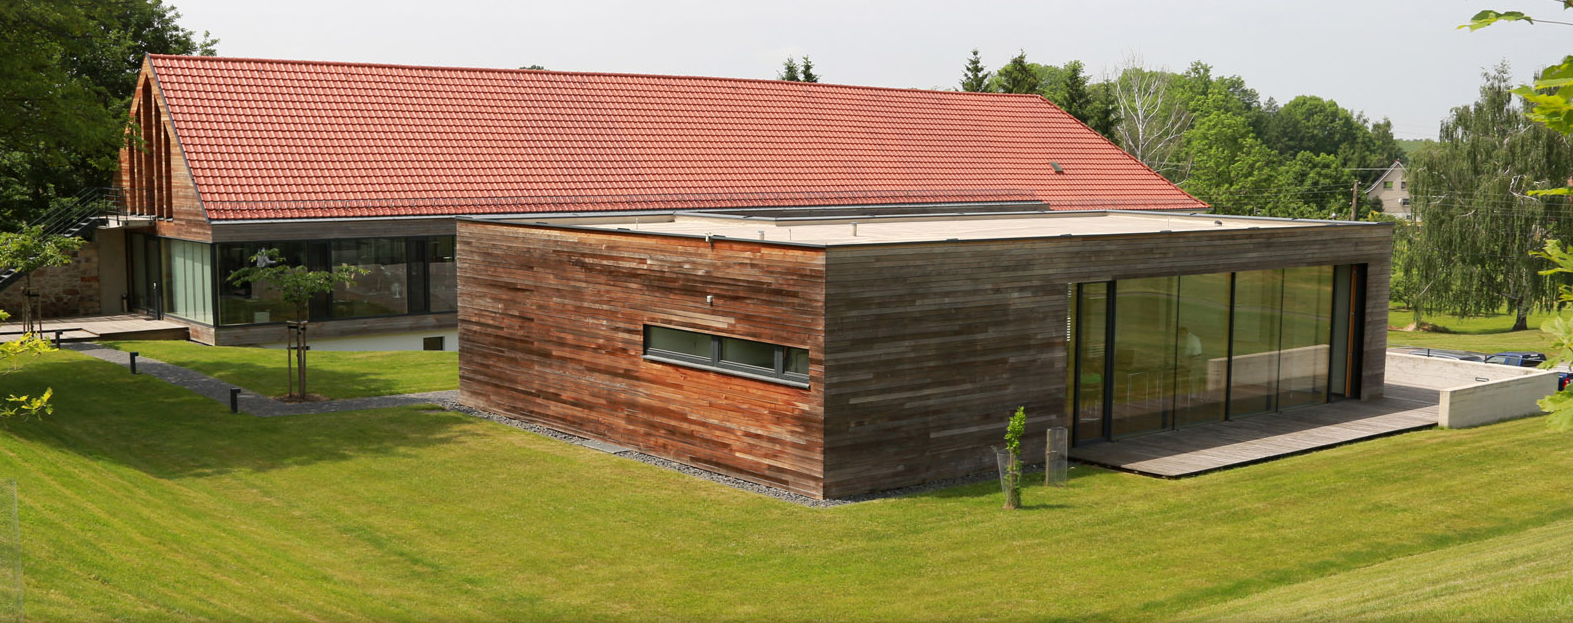
\includegraphics[scale=0.21]{Firma.png}
\end{wrapfigure}
\underline{Unternehmen:}\\
Agri Con GmbH\\\url{http://agricon.de}\\
% Datenerfassung über Sensoren und Probenahmegräte 
% Technik (Elekktronik) und Erfahrungen
% Einsatzplanung von Maschinen, Betriebsmitteln und Arbeitszeit
% EInklang von Ertrags- und Qualitätsziele mit den wachsenden Umweltanforderungen
% Sensoren, GPS, Terminal, Telemetrie, Datenmanegement, Grunddüngung
\vspace{\baselineskip}
\vspace{\baselineskip}
\textit{Precision Farming}
\end{frame}

\begin{frame}\frametitle{Einleitung}
%TODO Abbildung von Anje
\begin{figure}
\centering
% Graphic for TeX using PGF
% Title: C:\Masterthesis\masterthesis\Abbildungen\Ist-Stand.dia
% Creator: Dia v0.97.2
% CreationDate: Thu Jan 22 16:24:29 2015
% For: KJunghanns
% \usepackage{tikz}
% The following commands are not supported in PSTricks at present
% We define them conditionally, so when they are implemented,
% this pgf file will use them.
\ifx\du\undefined
  \newlength{\du}
\fi
\setlength{\du}{15\unitlength}
\begin{tikzpicture}
\pgftransformxscale{1.000000}
\pgftransformyscale{-1.000000}
\definecolor{dialinecolor}{rgb}{0.000000, 0.000000, 0.000000}
\pgfsetstrokecolor{dialinecolor}
\definecolor{dialinecolor}{rgb}{1.000000, 1.000000, 1.000000}
\pgfsetfillcolor{dialinecolor}
\pgfsetlinewidth{0.080000\du}
\pgfsetdash{}{0pt}
\pgfsetdash{}{0pt}
\pgfsetbuttcap
\pgfsetmiterjoin
\pgfsetlinewidth{0.080000\du}
\pgfsetbuttcap
\pgfsetmiterjoin
\pgfsetdash{}{0pt}
\definecolor{dialinecolor}{rgb}{1.000000, 1.000000, 1.000000}
\pgfsetfillcolor{dialinecolor}
\pgfpathmoveto{\pgfpoint{18.749943\du}{9.336199\du}}
\pgfpathcurveto{\pgfpoint{17.508208\du}{9.323238\du}}{\pgfpoint{15.100000\du}{9.595408\du}}{\pgfpoint{15.438655\du}{10.178627\du}}
\pgfpathcurveto{\pgfpoint{15.777306\du}{10.761847\du}}{\pgfpoint{17.395323\du}{10.891446\du}}{\pgfpoint{18.072633\du}{10.722966\du}}
\pgfpathcurveto{\pgfpoint{18.749943\du}{10.554480\du}}{\pgfpoint{17.019040\du}{11.539468\du}}{\pgfpoint{20.330332\du}{11.798677\du}}
\pgfpathcurveto{\pgfpoint{23.641594\du}{12.057885\du}}{\pgfpoint{25.334868\du}{11.643151\du}}{\pgfpoint{24.845700\du}{11.345061\du}}
\pgfpathcurveto{\pgfpoint{24.356532\du}{11.046971\du}}{\pgfpoint{27.743080\du}{12.044925\du}}{\pgfpoint{29.323469\du}{11.474666\du}}
\pgfpathcurveto{\pgfpoint{30.903858\du}{10.904406\du}}{\pgfpoint{27.705452\du}{10.360073\du}}{\pgfpoint{28.382761\du}{10.437836\du}}
\pgfpathcurveto{\pgfpoint{29.060071\du}{10.515599\du}}{\pgfpoint{31.129628\du}{10.411915\du}}{\pgfpoint{30.452319\du}{9.439882\du}}
\pgfpathcurveto{\pgfpoint{29.775009\du}{8.467850\du}}{\pgfpoint{23.679222\du}{9.219555\du}}{\pgfpoint{24.356532\du}{9.076990\du}}
\pgfpathcurveto{\pgfpoint{25.033841\du}{8.934425\du}}{\pgfpoint{23.340567\du}{8.221600\du}}{\pgfpoint{21.233412\du}{8.364165\du}}
\pgfpathcurveto{\pgfpoint{19.126226\du}{8.506731\du}}{\pgfpoint{18.976766\du}{8.765434\du}}{\pgfpoint{18.750996\du}{9.335693\du}}
\pgfpathlineto{\pgfpoint{18.749943\du}{9.336199\du}}
\pgfusepath{fill}
\definecolor{dialinecolor}{rgb}{0.000000, 0.000000, 0.000000}
\pgfsetstrokecolor{dialinecolor}
\pgfpathmoveto{\pgfpoint{18.749943\du}{9.336199\du}}
\pgfpathcurveto{\pgfpoint{17.508208\du}{9.323238\du}}{\pgfpoint{15.100000\du}{9.595408\du}}{\pgfpoint{15.438655\du}{10.178627\du}}
\pgfpathcurveto{\pgfpoint{15.777306\du}{10.761847\du}}{\pgfpoint{17.395323\du}{10.891446\du}}{\pgfpoint{18.072633\du}{10.722966\du}}
\pgfpathcurveto{\pgfpoint{18.749943\du}{10.554480\du}}{\pgfpoint{17.019040\du}{11.539468\du}}{\pgfpoint{20.330332\du}{11.798677\du}}
\pgfpathcurveto{\pgfpoint{23.641594\du}{12.057885\du}}{\pgfpoint{25.334868\du}{11.643151\du}}{\pgfpoint{24.845700\du}{11.345061\du}}
\pgfpathcurveto{\pgfpoint{24.356532\du}{11.046971\du}}{\pgfpoint{27.743080\du}{12.044925\du}}{\pgfpoint{29.323469\du}{11.474666\du}}
\pgfpathcurveto{\pgfpoint{30.903858\du}{10.904406\du}}{\pgfpoint{27.705452\du}{10.360073\du}}{\pgfpoint{28.382761\du}{10.437836\du}}
\pgfpathcurveto{\pgfpoint{29.060071\du}{10.515599\du}}{\pgfpoint{31.129628\du}{10.411915\du}}{\pgfpoint{30.452319\du}{9.439882\du}}
\pgfpathcurveto{\pgfpoint{29.775009\du}{8.467850\du}}{\pgfpoint{23.679222\du}{9.219555\du}}{\pgfpoint{24.356532\du}{9.076990\du}}
\pgfpathcurveto{\pgfpoint{25.033841\du}{8.934425\du}}{\pgfpoint{23.340567\du}{8.221600\du}}{\pgfpoint{21.233412\du}{8.364165\du}}
\pgfpathcurveto{\pgfpoint{19.126226\du}{8.506731\du}}{\pgfpoint{18.976766\du}{8.765434\du}}{\pgfpoint{18.750996\du}{9.335693\du}}
\pgfpathlineto{\pgfpoint{18.749943\du}{9.336199\du}}
\pgfusepath{stroke}
% setfont left to latex
\definecolor{dialinecolor}{rgb}{0.000000, 0.000000, 0.000000}
\pgfsetstrokecolor{dialinecolor}
\node at (23.544513\du,10.079368\du){Sensoren, externe Unternehmen,};
% setfont left to latex
\definecolor{dialinecolor}{rgb}{0.000000, 0.000000, 0.000000}
\pgfsetstrokecolor{dialinecolor}
\node at (23.544513\du,10.719368\du){Mitarbeiter};
\pgfsetlinewidth{0.080000\du}
\pgfsetdash{}{0pt}
\pgfsetdash{}{0pt}
\pgfsetbuttcap
\pgfsetmiterjoin
\pgfsetlinewidth{0.080000\du}
\pgfsetbuttcap
\pgfsetmiterjoin
\pgfsetdash{}{0pt}
\definecolor{dialinecolor}{rgb}{1.000000, 1.000000, 1.000000}
\pgfsetfillcolor{dialinecolor}
\fill (22.430000\du,14.010000\du)--(22.430000\du,15.210000\du)--(23.790000\du,15.210000\du)--(23.790000\du,14.010000\du)--cycle;
\pgfsetbuttcap
\pgfsetmiterjoin
\pgfsetdash{}{0pt}
\definecolor{dialinecolor}{rgb}{1.000000, 1.000000, 1.000000}
\pgfsetfillcolor{dialinecolor}
\pgfpathellipse{\pgfpoint{23.110000\du}{15.210000\du}}{\pgfpoint{0.680000\du}{0\du}}{\pgfpoint{0\du}{0.200000\du}}
\pgfusepath{fill}
\pgfsetbuttcap
\pgfsetmiterjoin
\pgfsetdash{}{0pt}
\definecolor{dialinecolor}{rgb}{1.000000, 1.000000, 1.000000}
\pgfsetfillcolor{dialinecolor}
\pgfpathellipse{\pgfpoint{23.110000\du}{14.010000\du}}{\pgfpoint{0.680000\du}{0\du}}{\pgfpoint{0\du}{0.200000\du}}
\pgfusepath{fill}
\definecolor{dialinecolor}{rgb}{0.000000, 0.000000, 0.000000}
\pgfsetstrokecolor{dialinecolor}
\pgfpathellipse{\pgfpoint{23.110000\du}{14.010000\du}}{\pgfpoint{0.680000\du}{0\du}}{\pgfpoint{0\du}{0.200000\du}}
\pgfusepath{stroke}
\pgfsetbuttcap
\pgfsetmiterjoin
\pgfsetdash{}{0pt}
\definecolor{dialinecolor}{rgb}{0.000000, 0.000000, 0.000000}
\pgfsetstrokecolor{dialinecolor}
\pgfpathmoveto{\pgfpoint{23.790000\du}{14.010000\du}}
\pgfpathlineto{\pgfpoint{23.790000\du}{15.210000\du}}
\pgfpathcurveto{\pgfpoint{23.790000\du}{15.320457\du}}{\pgfpoint{23.485554\du}{15.410000\du}}{\pgfpoint{23.110000\du}{15.410000\du}}
\pgfpathcurveto{\pgfpoint{22.734446\du}{15.410000\du}}{\pgfpoint{22.430000\du}{15.320457\du}}{\pgfpoint{22.430000\du}{15.210000\du}}
\pgfpathlineto{\pgfpoint{22.430000\du}{14.010000\du}}
\pgfusepath{stroke}
% setfont left to latex
\definecolor{dialinecolor}{rgb}{0.000000, 0.000000, 0.000000}
\pgfsetstrokecolor{dialinecolor}
\node at (23.110000\du,15.922000\du){PostgreSQL};
\pgfsetlinewidth{0.080000\du}
\pgfsetdash{}{0pt}
\pgfsetdash{}{0pt}
\pgfsetbuttcap
\pgfsetmiterjoin
\pgfsetlinewidth{0.040000\du}
\pgfsetbuttcap
\pgfsetmiterjoin
\pgfsetdash{}{0pt}
\definecolor{dialinecolor}{rgb}{0.701961, 0.701961, 0.701961}
\pgfsetfillcolor{dialinecolor}
\fill (22.416500\du,18.250000\du)--(22.416500\du,19.470339\du)--(24.043619\du,19.470339\du)--(24.043619\du,18.250000\du)--cycle;
\definecolor{dialinecolor}{rgb}{0.000000, 0.000000, 0.000000}
\pgfsetstrokecolor{dialinecolor}
\draw (22.416500\du,18.250000\du)--(22.416500\du,19.470339\du)--(24.043619\du,19.470339\du)--(24.043619\du,18.250000\du)--cycle;
\pgfsetlinewidth{0.080000\du}
\pgfsetbuttcap
\pgfsetmiterjoin
\pgfsetdash{}{0pt}
\definecolor{dialinecolor}{rgb}{0.000000, 0.000000, 0.000000}
\pgfsetfillcolor{dialinecolor}
\fill (22.592771\du,18.426271\du)--(22.592771\du,19.266949\du)--(23.867347\du,19.266949\du)--(23.867347\du,18.426271\du)--cycle;
\pgfsetlinewidth{0.040000\du}
\pgfsetbuttcap
\pgfsetmiterjoin
\pgfsetdash{}{0pt}
\definecolor{dialinecolor}{rgb}{0.701961, 0.701961, 0.701961}
\pgfsetfillcolor{dialinecolor}
\fill (22.636839\du,19.470339\du)--(23.474127\du,19.470339\du)--(23.474127\du,19.660169\du)--(22.680907\du,19.660169\du)--cycle;
\definecolor{dialinecolor}{rgb}{0.000000, 0.000000, 0.000000}
\pgfsetstrokecolor{dialinecolor}
\draw (22.636839\du,19.470339\du)--(23.474127\du,19.470339\du)--(23.474127\du,19.660169\du)--(22.680907\du,19.660169\du)--cycle;
\pgfsetbuttcap
\pgfsetmiterjoin
\pgfsetdash{}{0pt}
\definecolor{dialinecolor}{rgb}{0.701961, 0.701961, 0.701961}
\pgfsetfillcolor{dialinecolor}
\fill (23.474127\du,19.470339\du)--(23.823280\du,19.470339\du)--(23.779212\du,19.660169\du)--(23.474127\du,19.660169\du)--cycle;
\definecolor{dialinecolor}{rgb}{0.000000, 0.000000, 0.000000}
\pgfsetstrokecolor{dialinecolor}
\draw (23.474127\du,19.470339\du)--(23.823280\du,19.470339\du)--(23.779212\du,19.660169\du)--(23.474127\du,19.660169\du)--cycle;
\pgfsetlinewidth{0.020000\du}
\pgfsetbuttcap
\pgfsetmiterjoin
\pgfsetdash{}{0pt}
\definecolor{dialinecolor}{rgb}{1.000000, 1.000000, 1.000000}
\pgfsetfillcolor{dialinecolor}
\fill (23.531076\du,19.527288\du)--(23.531076\du,19.603220\du)--(23.607008\du,19.603220\du)--(23.607008\du,19.527288\du)--cycle;
\definecolor{dialinecolor}{rgb}{0.000000, 0.000000, 0.000000}
\pgfsetstrokecolor{dialinecolor}
\draw (23.531076\du,19.527288\du)--(23.531076\du,19.603220\du)--(23.607008\du,19.603220\du)--(23.607008\du,19.527288\du)--cycle;
\pgfsetlinewidth{0.040000\du}
\pgfsetbuttcap
\pgfsetmiterjoin
\pgfsetdash{}{0pt}
\definecolor{dialinecolor}{rgb}{0.701961, 0.701961, 0.701961}
\pgfsetfillcolor{dialinecolor}
\fill (23.067347\du,19.660169\du)--(23.392771\du,19.660169\du)--(23.392771\du,19.755085\du)--(23.555483\du,19.755085\du)--(23.555483\du,19.850000\du)--(22.904636\du,19.850000\du)--(22.904636\du,19.755085\du)--(23.067347\du,19.755085\du)--cycle;
\definecolor{dialinecolor}{rgb}{0.000000, 0.000000, 0.000000}
\pgfsetstrokecolor{dialinecolor}
\draw (23.067347\du,19.660169\du)--(23.392771\du,19.660169\du)--(23.392771\du,19.755085\du)--(23.555483\du,19.755085\du)--(23.555483\du,19.850000\du)--(22.904636\du,19.850000\du)--(22.904636\du,19.755085\du)--(23.067347\du,19.755085\du)--cycle;
% setfont left to latex
\definecolor{dialinecolor}{rgb}{0.000000, 0.000000, 0.000000}
\pgfsetstrokecolor{dialinecolor}
\node at (23.230059\du,20.416237\du){Agriport};
\pgfsetlinewidth{0.080000\du}
\pgfsetdash{}{0pt}
\pgfsetdash{}{0pt}
\pgfsetbuttcap
\pgfsetmiterjoin
\pgfsetlinewidth{0.080000\du}
\pgfsetbuttcap
\pgfsetmiterjoin
\pgfsetdash{}{0pt}
\definecolor{dialinecolor}{rgb}{0.850980, 0.850980, 0.803922}
\pgfsetfillcolor{dialinecolor}
\fill (16.670000\du,12.730000\du)--(16.670000\du,13.580000\du)--(17.690000\du,13.580000\du)--(17.690000\du,12.730000\du)--cycle;
\definecolor{dialinecolor}{rgb}{0.000000, 0.000000, 0.000000}
\pgfsetstrokecolor{dialinecolor}
\draw (16.670000\du,12.730000\du)--(16.670000\du,13.580000\du)--(17.690000\du,13.580000\du)--(17.690000\du,12.730000\du)--cycle;
\pgfsetlinewidth{0.008000\du}
\pgfsetbuttcap
\pgfsetmiterjoin
\pgfsetdash{}{0pt}
\definecolor{dialinecolor}{rgb}{0.000000, 0.000000, 0.000000}
\pgfsetstrokecolor{dialinecolor}
\draw (16.670000\du,12.730000\du)--(16.670000\du,13.580000\du)--(17.690000\du,13.580000\du)--(17.690000\du,12.730000\du)--cycle;
\pgfsetlinewidth{0.080000\du}
\pgfsetbuttcap
\pgfsetmiterjoin
\pgfsetdash{}{0pt}
\definecolor{dialinecolor}{rgb}{0.631373, 0.631373, 0.631373}
\pgfsetfillcolor{dialinecolor}
\fill (16.726667\du,12.786667\du)--(16.726667\du,13.466667\du)--(17.633333\du,13.466667\du)--(17.633333\du,12.786667\du)--cycle;
\definecolor{dialinecolor}{rgb}{0.000000, 0.000000, 0.000000}
\pgfsetstrokecolor{dialinecolor}
\draw (16.726667\du,12.786667\du)--(16.726667\du,13.466667\du)--(17.633333\du,13.466667\du)--(17.633333\du,12.786667\du)--cycle;
\pgfsetlinewidth{0.008000\du}
\pgfsetbuttcap
\pgfsetmiterjoin
\pgfsetdash{}{0pt}
\definecolor{dialinecolor}{rgb}{0.000000, 0.000000, 0.000000}
\pgfsetstrokecolor{dialinecolor}
\draw (16.726667\du,12.786667\du)--(16.726667\du,13.466667\du)--(17.633333\du,13.466667\du)--(17.633333\du,12.786667\du)--cycle;
\pgfsetlinewidth{0.080000\du}
\pgfsetbuttcap
\pgfsetmiterjoin
\pgfsetdash{}{0pt}
\definecolor{dialinecolor}{rgb}{0.850980, 0.850980, 0.803922}
\pgfsetfillcolor{dialinecolor}
\fill (16.840000\du,13.580000\du)--(17.520000\du,13.580000\du)--(17.350000\du,13.636667\du)--(17.010000\du,13.636667\du)--cycle;
\definecolor{dialinecolor}{rgb}{0.000000, 0.000000, 0.000000}
\pgfsetstrokecolor{dialinecolor}
\draw (16.840000\du,13.580000\du)--(17.520000\du,13.580000\du)--(17.350000\du,13.636667\du)--(17.010000\du,13.636667\du)--cycle;
\pgfsetlinewidth{0.008000\du}
\pgfsetbuttcap
\pgfsetmiterjoin
\pgfsetdash{}{0pt}
\definecolor{dialinecolor}{rgb}{0.000000, 0.000000, 0.000000}
\pgfsetstrokecolor{dialinecolor}
\draw (16.840000\du,13.580000\du)--(17.520000\du,13.580000\du)--(17.350000\du,13.636667\du)--(17.010000\du,13.636667\du)--cycle;
\pgfsetlinewidth{0.080000\du}
\pgfsetbuttcap
\pgfsetmiterjoin
\pgfsetdash{}{0pt}
\definecolor{dialinecolor}{rgb}{0.850980, 0.850980, 0.803922}
\pgfsetfillcolor{dialinecolor}
\fill (17.010000\du,13.636667\du)--(17.010000\du,13.693333\du)--(17.350000\du,13.693333\du)--(17.350000\du,13.636667\du)--cycle;
\definecolor{dialinecolor}{rgb}{0.000000, 0.000000, 0.000000}
\pgfsetstrokecolor{dialinecolor}
\draw (17.010000\du,13.636667\du)--(17.010000\du,13.693333\du)--(17.350000\du,13.693333\du)--(17.350000\du,13.636667\du)--cycle;
\pgfsetlinewidth{0.008000\du}
\pgfsetbuttcap
\pgfsetmiterjoin
\pgfsetdash{}{0pt}
\definecolor{dialinecolor}{rgb}{0.000000, 0.000000, 0.000000}
\pgfsetstrokecolor{dialinecolor}
\draw (17.010000\du,13.636667\du)--(17.010000\du,13.693333\du)--(17.350000\du,13.693333\du)--(17.350000\du,13.636667\du)--cycle;
\pgfsetlinewidth{0.080000\du}
\pgfsetbuttcap
\pgfsetmiterjoin
\pgfsetdash{}{0pt}
\definecolor{dialinecolor}{rgb}{0.850980, 0.850980, 0.803922}
\pgfsetfillcolor{dialinecolor}
\fill (16.840000\du,13.693333\du)--(16.840000\du,13.750000\du)--(17.520000\du,13.750000\du)--(17.520000\du,13.693333\du)--cycle;
\definecolor{dialinecolor}{rgb}{0.000000, 0.000000, 0.000000}
\pgfsetstrokecolor{dialinecolor}
\draw (16.840000\du,13.693333\du)--(16.840000\du,13.750000\du)--(17.520000\du,13.750000\du)--(17.520000\du,13.693333\du)--cycle;
\pgfsetlinewidth{0.008000\du}
\pgfsetbuttcap
\pgfsetmiterjoin
\pgfsetdash{}{0pt}
\definecolor{dialinecolor}{rgb}{0.000000, 0.000000, 0.000000}
\pgfsetstrokecolor{dialinecolor}
\draw (16.840000\du,13.693333\du)--(16.840000\du,13.750000\du)--(17.520000\du,13.750000\du)--(17.520000\du,13.693333\du)--cycle;
\pgfsetlinewidth{0.080000\du}
\pgfsetdash{}{0pt}
\pgfsetdash{}{0pt}
\pgfsetbuttcap
\pgfsetmiterjoin
\pgfsetlinewidth{0.080000\du}
\pgfsetbuttcap
\pgfsetmiterjoin
\pgfsetdash{}{0pt}
\definecolor{dialinecolor}{rgb}{0.850980, 0.850980, 0.803922}
\pgfsetfillcolor{dialinecolor}
\fill (17.498500\du,14.398000\du)--(17.498500\du,15.248000\du)--(18.518500\du,15.248000\du)--(18.518500\du,14.398000\du)--cycle;
\definecolor{dialinecolor}{rgb}{0.000000, 0.000000, 0.000000}
\pgfsetstrokecolor{dialinecolor}
\draw (17.498500\du,14.398000\du)--(17.498500\du,15.248000\du)--(18.518500\du,15.248000\du)--(18.518500\du,14.398000\du)--cycle;
\pgfsetlinewidth{0.008000\du}
\pgfsetbuttcap
\pgfsetmiterjoin
\pgfsetdash{}{0pt}
\definecolor{dialinecolor}{rgb}{0.000000, 0.000000, 0.000000}
\pgfsetstrokecolor{dialinecolor}
\draw (17.498500\du,14.398000\du)--(17.498500\du,15.248000\du)--(18.518500\du,15.248000\du)--(18.518500\du,14.398000\du)--cycle;
\pgfsetlinewidth{0.080000\du}
\pgfsetbuttcap
\pgfsetmiterjoin
\pgfsetdash{}{0pt}
\definecolor{dialinecolor}{rgb}{0.631373, 0.631373, 0.631373}
\pgfsetfillcolor{dialinecolor}
\fill (17.555167\du,14.454667\du)--(17.555167\du,15.134667\du)--(18.461833\du,15.134667\du)--(18.461833\du,14.454667\du)--cycle;
\definecolor{dialinecolor}{rgb}{0.000000, 0.000000, 0.000000}
\pgfsetstrokecolor{dialinecolor}
\draw (17.555167\du,14.454667\du)--(17.555167\du,15.134667\du)--(18.461833\du,15.134667\du)--(18.461833\du,14.454667\du)--cycle;
\pgfsetlinewidth{0.008000\du}
\pgfsetbuttcap
\pgfsetmiterjoin
\pgfsetdash{}{0pt}
\definecolor{dialinecolor}{rgb}{0.000000, 0.000000, 0.000000}
\pgfsetstrokecolor{dialinecolor}
\draw (17.555167\du,14.454667\du)--(17.555167\du,15.134667\du)--(18.461833\du,15.134667\du)--(18.461833\du,14.454667\du)--cycle;
\pgfsetlinewidth{0.080000\du}
\pgfsetbuttcap
\pgfsetmiterjoin
\pgfsetdash{}{0pt}
\definecolor{dialinecolor}{rgb}{0.850980, 0.850980, 0.803922}
\pgfsetfillcolor{dialinecolor}
\fill (17.668500\du,15.248000\du)--(18.348500\du,15.248000\du)--(18.178500\du,15.304667\du)--(17.838500\du,15.304667\du)--cycle;
\definecolor{dialinecolor}{rgb}{0.000000, 0.000000, 0.000000}
\pgfsetstrokecolor{dialinecolor}
\draw (17.668500\du,15.248000\du)--(18.348500\du,15.248000\du)--(18.178500\du,15.304667\du)--(17.838500\du,15.304667\du)--cycle;
\pgfsetlinewidth{0.008000\du}
\pgfsetbuttcap
\pgfsetmiterjoin
\pgfsetdash{}{0pt}
\definecolor{dialinecolor}{rgb}{0.000000, 0.000000, 0.000000}
\pgfsetstrokecolor{dialinecolor}
\draw (17.668500\du,15.248000\du)--(18.348500\du,15.248000\du)--(18.178500\du,15.304667\du)--(17.838500\du,15.304667\du)--cycle;
\pgfsetlinewidth{0.080000\du}
\pgfsetbuttcap
\pgfsetmiterjoin
\pgfsetdash{}{0pt}
\definecolor{dialinecolor}{rgb}{0.850980, 0.850980, 0.803922}
\pgfsetfillcolor{dialinecolor}
\fill (17.838500\du,15.304667\du)--(17.838500\du,15.361333\du)--(18.178500\du,15.361333\du)--(18.178500\du,15.304667\du)--cycle;
\definecolor{dialinecolor}{rgb}{0.000000, 0.000000, 0.000000}
\pgfsetstrokecolor{dialinecolor}
\draw (17.838500\du,15.304667\du)--(17.838500\du,15.361333\du)--(18.178500\du,15.361333\du)--(18.178500\du,15.304667\du)--cycle;
\pgfsetlinewidth{0.008000\du}
\pgfsetbuttcap
\pgfsetmiterjoin
\pgfsetdash{}{0pt}
\definecolor{dialinecolor}{rgb}{0.000000, 0.000000, 0.000000}
\pgfsetstrokecolor{dialinecolor}
\draw (17.838500\du,15.304667\du)--(17.838500\du,15.361333\du)--(18.178500\du,15.361333\du)--(18.178500\du,15.304667\du)--cycle;
\pgfsetlinewidth{0.080000\du}
\pgfsetbuttcap
\pgfsetmiterjoin
\pgfsetdash{}{0pt}
\definecolor{dialinecolor}{rgb}{0.850980, 0.850980, 0.803922}
\pgfsetfillcolor{dialinecolor}
\fill (17.668500\du,15.361333\du)--(17.668500\du,15.418000\du)--(18.348500\du,15.418000\du)--(18.348500\du,15.361333\du)--cycle;
\definecolor{dialinecolor}{rgb}{0.000000, 0.000000, 0.000000}
\pgfsetstrokecolor{dialinecolor}
\draw (17.668500\du,15.361333\du)--(17.668500\du,15.418000\du)--(18.348500\du,15.418000\du)--(18.348500\du,15.361333\du)--cycle;
\pgfsetlinewidth{0.008000\du}
\pgfsetbuttcap
\pgfsetmiterjoin
\pgfsetdash{}{0pt}
\definecolor{dialinecolor}{rgb}{0.000000, 0.000000, 0.000000}
\pgfsetstrokecolor{dialinecolor}
\draw (17.668500\du,15.361333\du)--(17.668500\du,15.418000\du)--(18.348500\du,15.418000\du)--(18.348500\du,15.361333\du)--cycle;
\pgfsetlinewidth{0.080000\du}
\pgfsetdash{}{0pt}
\pgfsetdash{}{0pt}
\pgfsetbuttcap
\pgfsetmiterjoin
\pgfsetlinewidth{0.080000\du}
\pgfsetbuttcap
\pgfsetmiterjoin
\pgfsetdash{}{0pt}
\definecolor{dialinecolor}{rgb}{0.850980, 0.850980, 0.803922}
\pgfsetfillcolor{dialinecolor}
\fill (16.770500\du,15.946000\du)--(16.770500\du,16.796000\du)--(17.790500\du,16.796000\du)--(17.790500\du,15.946000\du)--cycle;
\definecolor{dialinecolor}{rgb}{0.000000, 0.000000, 0.000000}
\pgfsetstrokecolor{dialinecolor}
\draw (16.770500\du,15.946000\du)--(16.770500\du,16.796000\du)--(17.790500\du,16.796000\du)--(17.790500\du,15.946000\du)--cycle;
\pgfsetlinewidth{0.008000\du}
\pgfsetbuttcap
\pgfsetmiterjoin
\pgfsetdash{}{0pt}
\definecolor{dialinecolor}{rgb}{0.000000, 0.000000, 0.000000}
\pgfsetstrokecolor{dialinecolor}
\draw (16.770500\du,15.946000\du)--(16.770500\du,16.796000\du)--(17.790500\du,16.796000\du)--(17.790500\du,15.946000\du)--cycle;
\pgfsetlinewidth{0.080000\du}
\pgfsetbuttcap
\pgfsetmiterjoin
\pgfsetdash{}{0pt}
\definecolor{dialinecolor}{rgb}{0.631373, 0.631373, 0.631373}
\pgfsetfillcolor{dialinecolor}
\fill (16.827167\du,16.002667\du)--(16.827167\du,16.682667\du)--(17.733833\du,16.682667\du)--(17.733833\du,16.002667\du)--cycle;
\definecolor{dialinecolor}{rgb}{0.000000, 0.000000, 0.000000}
\pgfsetstrokecolor{dialinecolor}
\draw (16.827167\du,16.002667\du)--(16.827167\du,16.682667\du)--(17.733833\du,16.682667\du)--(17.733833\du,16.002667\du)--cycle;
\pgfsetlinewidth{0.008000\du}
\pgfsetbuttcap
\pgfsetmiterjoin
\pgfsetdash{}{0pt}
\definecolor{dialinecolor}{rgb}{0.000000, 0.000000, 0.000000}
\pgfsetstrokecolor{dialinecolor}
\draw (16.827167\du,16.002667\du)--(16.827167\du,16.682667\du)--(17.733833\du,16.682667\du)--(17.733833\du,16.002667\du)--cycle;
\pgfsetlinewidth{0.080000\du}
\pgfsetbuttcap
\pgfsetmiterjoin
\pgfsetdash{}{0pt}
\definecolor{dialinecolor}{rgb}{0.850980, 0.850980, 0.803922}
\pgfsetfillcolor{dialinecolor}
\fill (16.940500\du,16.796000\du)--(17.620500\du,16.796000\du)--(17.450500\du,16.852667\du)--(17.110500\du,16.852667\du)--cycle;
\definecolor{dialinecolor}{rgb}{0.000000, 0.000000, 0.000000}
\pgfsetstrokecolor{dialinecolor}
\draw (16.940500\du,16.796000\du)--(17.620500\du,16.796000\du)--(17.450500\du,16.852667\du)--(17.110500\du,16.852667\du)--cycle;
\pgfsetlinewidth{0.008000\du}
\pgfsetbuttcap
\pgfsetmiterjoin
\pgfsetdash{}{0pt}
\definecolor{dialinecolor}{rgb}{0.000000, 0.000000, 0.000000}
\pgfsetstrokecolor{dialinecolor}
\draw (16.940500\du,16.796000\du)--(17.620500\du,16.796000\du)--(17.450500\du,16.852667\du)--(17.110500\du,16.852667\du)--cycle;
\pgfsetlinewidth{0.080000\du}
\pgfsetbuttcap
\pgfsetmiterjoin
\pgfsetdash{}{0pt}
\definecolor{dialinecolor}{rgb}{0.850980, 0.850980, 0.803922}
\pgfsetfillcolor{dialinecolor}
\fill (17.110500\du,16.852667\du)--(17.110500\du,16.909333\du)--(17.450500\du,16.909333\du)--(17.450500\du,16.852667\du)--cycle;
\definecolor{dialinecolor}{rgb}{0.000000, 0.000000, 0.000000}
\pgfsetstrokecolor{dialinecolor}
\draw (17.110500\du,16.852667\du)--(17.110500\du,16.909333\du)--(17.450500\du,16.909333\du)--(17.450500\du,16.852667\du)--cycle;
\pgfsetlinewidth{0.008000\du}
\pgfsetbuttcap
\pgfsetmiterjoin
\pgfsetdash{}{0pt}
\definecolor{dialinecolor}{rgb}{0.000000, 0.000000, 0.000000}
\pgfsetstrokecolor{dialinecolor}
\draw (17.110500\du,16.852667\du)--(17.110500\du,16.909333\du)--(17.450500\du,16.909333\du)--(17.450500\du,16.852667\du)--cycle;
\pgfsetlinewidth{0.080000\du}
\pgfsetbuttcap
\pgfsetmiterjoin
\pgfsetdash{}{0pt}
\definecolor{dialinecolor}{rgb}{0.850980, 0.850980, 0.803922}
\pgfsetfillcolor{dialinecolor}
\fill (16.940500\du,16.909333\du)--(16.940500\du,16.966000\du)--(17.620500\du,16.966000\du)--(17.620500\du,16.909333\du)--cycle;
\definecolor{dialinecolor}{rgb}{0.000000, 0.000000, 0.000000}
\pgfsetstrokecolor{dialinecolor}
\draw (16.940500\du,16.909333\du)--(16.940500\du,16.966000\du)--(17.620500\du,16.966000\du)--(17.620500\du,16.909333\du)--cycle;
\pgfsetlinewidth{0.008000\du}
\pgfsetbuttcap
\pgfsetmiterjoin
\pgfsetdash{}{0pt}
\definecolor{dialinecolor}{rgb}{0.000000, 0.000000, 0.000000}
\pgfsetstrokecolor{dialinecolor}
\draw (16.940500\du,16.909333\du)--(16.940500\du,16.966000\du)--(17.620500\du,16.966000\du)--(17.620500\du,16.909333\du)--cycle;
% setfont left to latex
\definecolor{dialinecolor}{rgb}{0.000000, 0.000000, 0.000000}
\pgfsetstrokecolor{dialinecolor}
\node[anchor=west] at (15.590000\du,17.730000\du){Agri Con Intern};
\pgfsetlinewidth{0.080000\du}
\pgfsetdash{}{0pt}
\pgfsetdash{}{0pt}
\pgfsetbuttcap
{
\definecolor{dialinecolor}{rgb}{0.000000, 0.000000, 0.000000}
\pgfsetfillcolor{dialinecolor}
% was here!!!
\pgfsetarrowsend{stealth}
\definecolor{dialinecolor}{rgb}{0.000000, 0.000000, 0.000000}
\pgfsetstrokecolor{dialinecolor}
\draw (23.167337\du,11.886149\du)--(23.210796\du,13.775218\du);
}
\pgfsetlinewidth{0.080000\du}
\pgfsetdash{}{0pt}
\pgfsetdash{}{0pt}
\pgfsetbuttcap
{
\definecolor{dialinecolor}{rgb}{0.000000, 0.000000, 0.000000}
\pgfsetfillcolor{dialinecolor}
% was here!!!
\pgfsetarrowsstart{stealth}
\pgfsetarrowsend{latex}
\definecolor{dialinecolor}{rgb}{0.000000, 0.000000, 0.000000}
\pgfsetstrokecolor{dialinecolor}
\draw (23.238032\du,16.373080\du)--(23.232496\du,18.231762\du);
}
\pgfsetlinewidth{0.080000\du}
\pgfsetdash{}{0pt}
\pgfsetdash{}{0pt}
\pgfsetbuttcap
{
\definecolor{dialinecolor}{rgb}{0.000000, 0.000000, 0.000000}
\pgfsetfillcolor{dialinecolor}
% was here!!!
\pgfsetarrowsstart{latex}
\pgfsetarrowsend{latex}
\definecolor{dialinecolor}{rgb}{0.000000, 0.000000, 0.000000}
\pgfsetstrokecolor{dialinecolor}
\draw (22.391973\du,14.610000\du)--(18.950000\du,14.610000\du);
}
\pgfsetlinewidth{0.080000\du}
\pgfsetdash{}{0pt}
\pgfsetdash{}{0pt}
\pgfsetbuttcap
{
\definecolor{dialinecolor}{rgb}{0.000000, 0.000000, 0.000000}
\pgfsetfillcolor{dialinecolor}
% was here!!!
\pgfsetarrowsend{latex}
\definecolor{dialinecolor}{rgb}{0.000000, 0.000000, 0.000000}
\pgfsetstrokecolor{dialinecolor}
\pgfpathmoveto{\pgfpoint{23.821525\du}{16.535113\du}}
\pgfpatharc{131}{-128}{1.640858\du and 1.640858\du}
\pgfusepath{stroke}
}
% setfont left to latex
\definecolor{dialinecolor}{rgb}{0.000000, 0.000000, 0.000000}
\pgfsetstrokecolor{dialinecolor}
\node[anchor=west] at (26.722640\du,14.883849\du){Batch};
% setfont left to latex
\definecolor{dialinecolor}{rgb}{0.000000, 0.000000, 0.000000}
\pgfsetstrokecolor{dialinecolor}
\node[anchor=west] at (26.722640\du,15.523849\du){Vorgänge};
\end{tikzpicture}

\caption{Aktueller Stand bei Agri Con}
\end{figure}
\end{frame}

\begin{frame}\frametitle{Einleitung}
%TODO Abbildung von Anje
\begin{figure}[h!]
\centering
\resizebox{.92\linewidth}{!}{% Graphic for TeX using PGF
% Title: C:\Masterthesis\masterthesis\Abbildungen\Wunsch-Stand.dia
% Creator: Dia v0.97.2
% CreationDate: Thu Jan 22 16:40:13 2015
% For: KJunghanns
% \usepackage{tikz}
% The following commands are not supported in PSTricks at present
% We define them conditionally, so when they are implemented,
% this pgf file will use them.
\ifx\du\undefined
  \newlength{\du}
\fi
\setlength{\du}{15\unitlength}
\begin{tikzpicture}
\pgftransformxscale{1.000000}
\pgftransformyscale{-1.000000}
\definecolor{dialinecolor}{rgb}{0.000000, 0.000000, 0.000000}
\pgfsetstrokecolor{dialinecolor}
\definecolor{dialinecolor}{rgb}{1.000000, 1.000000, 1.000000}
\pgfsetfillcolor{dialinecolor}
\pgfsetlinewidth{0.100000\du}
\pgfsetdash{}{0pt}
\pgfsetdash{}{0pt}
\pgfsetbuttcap
\pgfsetmiterjoin
\pgfsetlinewidth{0.100000\du}
\pgfsetbuttcap
\pgfsetmiterjoin
\pgfsetdash{}{0pt}
\definecolor{dialinecolor}{rgb}{1.000000, 1.000000, 1.000000}
\pgfsetfillcolor{dialinecolor}
\pgfpathmoveto{\pgfpoint{16.667981\du}{7.329099\du}}
\pgfpathcurveto{\pgfpoint{15.122429\du}{7.316138\du}}{\pgfpoint{12.125000\du}{7.588308\du}}{\pgfpoint{12.546514\du}{8.171527\du}}
\pgfpathcurveto{\pgfpoint{12.968024\du}{8.754747\du}}{\pgfpoint{14.981924\du}{8.884346\du}}{\pgfpoint{15.824953\du}{8.715866\du}}
\pgfpathcurveto{\pgfpoint{16.667981\du}{8.547380\du}}{\pgfpoint{14.513575\du}{9.532368\du}}{\pgfpoint{18.635047\du}{9.791577\du}}
\pgfpathcurveto{\pgfpoint{22.756481\du}{10.050785\du}}{\pgfpoint{24.864051\du}{9.636051\du}}{\pgfpoint{24.255197\du}{9.337961\du}}
\pgfpathcurveto{\pgfpoint{23.646344\du}{9.039871\du}}{\pgfpoint{27.861485\du}{10.037825\du}}{\pgfpoint{29.828551\du}{9.467566\du}}
\pgfpathcurveto{\pgfpoint{31.795617\du}{8.897306\du}}{\pgfpoint{27.814650\du}{8.352973\du}}{\pgfpoint{28.657678\du}{8.430736\du}}
\pgfpathcurveto{\pgfpoint{29.500706\du}{8.508499\du}}{\pgfpoint{32.076626\du}{8.404815\du}}{\pgfpoint{31.233598\du}{7.432782\du}}
\pgfpathcurveto{\pgfpoint{30.390569\du}{6.460750\du}}{\pgfpoint{22.803315\du}{7.212455\du}}{\pgfpoint{23.646344\du}{7.069890\du}}
\pgfpathcurveto{\pgfpoint{24.489372\du}{6.927325\du}}{\pgfpoint{22.381801\du}{6.214500\du}}{\pgfpoint{19.759084\du}{6.357065\du}}
\pgfpathcurveto{\pgfpoint{17.136330\du}{6.499631\du}}{\pgfpoint{16.950302\du}{6.758334\du}}{\pgfpoint{16.669292\du}{7.328593\du}}
\pgfpathlineto{\pgfpoint{16.667981\du}{7.329099\du}}
\pgfusepath{fill}
\definecolor{dialinecolor}{rgb}{0.000000, 0.000000, 0.000000}
\pgfsetstrokecolor{dialinecolor}
\pgfpathmoveto{\pgfpoint{16.667981\du}{7.329099\du}}
\pgfpathcurveto{\pgfpoint{15.122429\du}{7.316138\du}}{\pgfpoint{12.125000\du}{7.588308\du}}{\pgfpoint{12.546514\du}{8.171527\du}}
\pgfpathcurveto{\pgfpoint{12.968024\du}{8.754747\du}}{\pgfpoint{14.981924\du}{8.884346\du}}{\pgfpoint{15.824953\du}{8.715866\du}}
\pgfpathcurveto{\pgfpoint{16.667981\du}{8.547380\du}}{\pgfpoint{14.513575\du}{9.532368\du}}{\pgfpoint{18.635047\du}{9.791577\du}}
\pgfpathcurveto{\pgfpoint{22.756481\du}{10.050785\du}}{\pgfpoint{24.864051\du}{9.636051\du}}{\pgfpoint{24.255197\du}{9.337961\du}}
\pgfpathcurveto{\pgfpoint{23.646344\du}{9.039871\du}}{\pgfpoint{27.861485\du}{10.037825\du}}{\pgfpoint{29.828551\du}{9.467566\du}}
\pgfpathcurveto{\pgfpoint{31.795617\du}{8.897306\du}}{\pgfpoint{27.814650\du}{8.352973\du}}{\pgfpoint{28.657678\du}{8.430736\du}}
\pgfpathcurveto{\pgfpoint{29.500706\du}{8.508499\du}}{\pgfpoint{32.076626\du}{8.404815\du}}{\pgfpoint{31.233598\du}{7.432782\du}}
\pgfpathcurveto{\pgfpoint{30.390569\du}{6.460750\du}}{\pgfpoint{22.803315\du}{7.212455\du}}{\pgfpoint{23.646344\du}{7.069890\du}}
\pgfpathcurveto{\pgfpoint{24.489372\du}{6.927325\du}}{\pgfpoint{22.381801\du}{6.214500\du}}{\pgfpoint{19.759084\du}{6.357065\du}}
\pgfpathcurveto{\pgfpoint{17.136330\du}{6.499631\du}}{\pgfpoint{16.950302\du}{6.758334\du}}{\pgfpoint{16.669292\du}{7.328593\du}}
\pgfpathlineto{\pgfpoint{16.667981\du}{7.329099\du}}
\pgfusepath{stroke}
% setfont left to latex
\definecolor{dialinecolor}{rgb}{0.000000, 0.000000, 0.000000}
\pgfsetstrokecolor{dialinecolor}
\node at (22.635646\du,8.040268\du){Sensoren, externe Unternehmen,};
% setfont left to latex
\definecolor{dialinecolor}{rgb}{0.000000, 0.000000, 0.000000}
\pgfsetstrokecolor{dialinecolor}
\node at (22.635646\du,8.840268\du){Mitarbeiter};
\pgfsetlinewidth{0.100000\du}
\pgfsetdash{}{0pt}
\pgfsetdash{}{0pt}
\pgfsetbuttcap
\pgfsetmiterjoin
\pgfsetlinewidth{0.100000\du}
\pgfsetbuttcap
\pgfsetmiterjoin
\pgfsetdash{}{0pt}
\definecolor{dialinecolor}{rgb}{1.000000, 1.000000, 1.000000}
\pgfsetfillcolor{dialinecolor}
\fill (21.100000\du,13.450000\du)--(21.100000\du,14.950000\du)--(22.800000\du,14.950000\du)--(22.800000\du,13.450000\du)--cycle;
\pgfsetbuttcap
\pgfsetmiterjoin
\pgfsetdash{}{0pt}
\definecolor{dialinecolor}{rgb}{1.000000, 1.000000, 1.000000}
\pgfsetfillcolor{dialinecolor}
\pgfpathellipse{\pgfpoint{21.950000\du}{14.950000\du}}{\pgfpoint{0.850000\du}{0\du}}{\pgfpoint{0\du}{0.250000\du}}
\pgfusepath{fill}
\pgfsetbuttcap
\pgfsetmiterjoin
\pgfsetdash{}{0pt}
\definecolor{dialinecolor}{rgb}{1.000000, 1.000000, 1.000000}
\pgfsetfillcolor{dialinecolor}
\pgfpathellipse{\pgfpoint{21.950000\du}{13.450000\du}}{\pgfpoint{0.850000\du}{0\du}}{\pgfpoint{0\du}{0.250000\du}}
\pgfusepath{fill}
\definecolor{dialinecolor}{rgb}{0.000000, 0.000000, 0.000000}
\pgfsetstrokecolor{dialinecolor}
\pgfpathellipse{\pgfpoint{21.950000\du}{13.450000\du}}{\pgfpoint{0.850000\du}{0\du}}{\pgfpoint{0\du}{0.250000\du}}
\pgfusepath{stroke}
\pgfsetbuttcap
\pgfsetmiterjoin
\pgfsetdash{}{0pt}
\definecolor{dialinecolor}{rgb}{0.000000, 0.000000, 0.000000}
\pgfsetstrokecolor{dialinecolor}
\pgfpathmoveto{\pgfpoint{22.800000\du}{13.450000\du}}
\pgfpathlineto{\pgfpoint{22.800000\du}{14.950000\du}}
\pgfpathcurveto{\pgfpoint{22.800000\du}{15.088071\du}}{\pgfpoint{22.419442\du}{15.200000\du}}{\pgfpoint{21.950000\du}{15.200000\du}}
\pgfpathcurveto{\pgfpoint{21.480558\du}{15.200000\du}}{\pgfpoint{21.100000\du}{15.088071\du}}{\pgfpoint{21.100000\du}{14.950000\du}}
\pgfpathlineto{\pgfpoint{21.100000\du}{13.450000\du}}
\pgfusepath{stroke}
% setfont left to latex
\definecolor{dialinecolor}{rgb}{0.000000, 0.000000, 0.000000}
\pgfsetstrokecolor{dialinecolor}
\node at (21.950000\du,15.840000\du){PostgreSQL};
\pgfsetlinewidth{0.100000\du}
\pgfsetdash{}{0pt}
\pgfsetdash{}{0pt}
\pgfsetbuttcap
\pgfsetmiterjoin
\pgfsetlinewidth{0.050000\du}
\pgfsetbuttcap
\pgfsetmiterjoin
\pgfsetdash{}{0pt}
\definecolor{dialinecolor}{rgb}{0.701961, 0.701961, 0.701961}
\pgfsetfillcolor{dialinecolor}
\fill (21.083100\du,18.750000\du)--(21.083100\du,20.275424\du)--(23.116998\du,20.275424\du)--(23.116998\du,18.750000\du)--cycle;
\definecolor{dialinecolor}{rgb}{0.000000, 0.000000, 0.000000}
\pgfsetstrokecolor{dialinecolor}
\draw (21.083100\du,18.750000\du)--(21.083100\du,20.275424\du)--(23.116998\du,20.275424\du)--(23.116998\du,18.750000\du)--cycle;
\pgfsetlinewidth{0.100000\du}
\pgfsetbuttcap
\pgfsetmiterjoin
\pgfsetdash{}{0pt}
\definecolor{dialinecolor}{rgb}{0.000000, 0.000000, 0.000000}
\pgfsetfillcolor{dialinecolor}
\fill (21.303439\du,18.970339\du)--(21.303439\du,20.021186\du)--(22.896659\du,20.021186\du)--(22.896659\du,18.970339\du)--cycle;
\pgfsetlinewidth{0.050000\du}
\pgfsetbuttcap
\pgfsetmiterjoin
\pgfsetdash{}{0pt}
\definecolor{dialinecolor}{rgb}{0.701961, 0.701961, 0.701961}
\pgfsetfillcolor{dialinecolor}
\fill (21.358524\du,20.275424\du)--(22.405134\du,20.275424\du)--(22.405134\du,20.512712\du)--(21.413608\du,20.512712\du)--cycle;
\definecolor{dialinecolor}{rgb}{0.000000, 0.000000, 0.000000}
\pgfsetstrokecolor{dialinecolor}
\draw (21.358524\du,20.275424\du)--(22.405134\du,20.275424\du)--(22.405134\du,20.512712\du)--(21.413608\du,20.512712\du)--cycle;
\pgfsetbuttcap
\pgfsetmiterjoin
\pgfsetdash{}{0pt}
\definecolor{dialinecolor}{rgb}{0.701961, 0.701961, 0.701961}
\pgfsetfillcolor{dialinecolor}
\fill (22.405134\du,20.275424\du)--(22.841575\du,20.275424\du)--(22.786490\du,20.512712\du)--(22.405134\du,20.512712\du)--cycle;
\definecolor{dialinecolor}{rgb}{0.000000, 0.000000, 0.000000}
\pgfsetstrokecolor{dialinecolor}
\draw (22.405134\du,20.275424\du)--(22.841575\du,20.275424\du)--(22.786490\du,20.512712\du)--(22.405134\du,20.512712\du)--cycle;
\pgfsetlinewidth{0.025000\du}
\pgfsetbuttcap
\pgfsetmiterjoin
\pgfsetdash{}{0pt}
\definecolor{dialinecolor}{rgb}{1.000000, 1.000000, 1.000000}
\pgfsetfillcolor{dialinecolor}
\fill (22.476320\du,20.346610\du)--(22.476320\du,20.441525\du)--(22.571236\du,20.441525\du)--(22.571236\du,20.346610\du)--cycle;
\definecolor{dialinecolor}{rgb}{0.000000, 0.000000, 0.000000}
\pgfsetstrokecolor{dialinecolor}
\draw (22.476320\du,20.346610\du)--(22.476320\du,20.441525\du)--(22.571236\du,20.441525\du)--(22.571236\du,20.346610\du)--cycle;
\pgfsetlinewidth{0.050000\du}
\pgfsetbuttcap
\pgfsetmiterjoin
\pgfsetdash{}{0pt}
\definecolor{dialinecolor}{rgb}{0.701961, 0.701961, 0.701961}
\pgfsetfillcolor{dialinecolor}
\fill (21.896659\du,20.512712\du)--(22.303439\du,20.512712\du)--(22.303439\du,20.631356\du)--(22.506829\du,20.631356\du)--(22.506829\du,20.750000\du)--(21.693269\du,20.750000\du)--(21.693269\du,20.631356\du)--(21.896659\du,20.631356\du)--cycle;
\definecolor{dialinecolor}{rgb}{0.000000, 0.000000, 0.000000}
\pgfsetstrokecolor{dialinecolor}
\draw (21.896659\du,20.512712\du)--(22.303439\du,20.512712\du)--(22.303439\du,20.631356\du)--(22.506829\du,20.631356\du)--(22.506829\du,20.750000\du)--(21.693269\du,20.750000\du)--(21.693269\du,20.631356\du)--(21.896659\du,20.631356\du)--cycle;
% setfont left to latex
\definecolor{dialinecolor}{rgb}{0.000000, 0.000000, 0.000000}
\pgfsetstrokecolor{dialinecolor}
\node at (22.100049\du,21.457797\du){Agriport};
\pgfsetlinewidth{0.100000\du}
\pgfsetdash{}{0pt}
\pgfsetdash{}{0pt}
\pgfsetbuttcap
\pgfsetmiterjoin
\pgfsetlinewidth{0.100000\du}
\pgfsetbuttcap
\pgfsetmiterjoin
\pgfsetdash{}{0pt}
\definecolor{dialinecolor}{rgb}{0.850980, 0.850980, 0.803922}
\pgfsetfillcolor{dialinecolor}
\fill (13.900000\du,11.850000\du)--(13.900000\du,12.912500\du)--(15.175000\du,12.912500\du)--(15.175000\du,11.850000\du)--cycle;
\definecolor{dialinecolor}{rgb}{0.000000, 0.000000, 0.000000}
\pgfsetstrokecolor{dialinecolor}
\draw (13.900000\du,11.850000\du)--(13.900000\du,12.912500\du)--(15.175000\du,12.912500\du)--(15.175000\du,11.850000\du)--cycle;
\pgfsetlinewidth{0.010000\du}
\pgfsetbuttcap
\pgfsetmiterjoin
\pgfsetdash{}{0pt}
\definecolor{dialinecolor}{rgb}{0.000000, 0.000000, 0.000000}
\pgfsetstrokecolor{dialinecolor}
\draw (13.900000\du,11.850000\du)--(13.900000\du,12.912500\du)--(15.175000\du,12.912500\du)--(15.175000\du,11.850000\du)--cycle;
\pgfsetlinewidth{0.100000\du}
\pgfsetbuttcap
\pgfsetmiterjoin
\pgfsetdash{}{0pt}
\definecolor{dialinecolor}{rgb}{0.631373, 0.631373, 0.631373}
\pgfsetfillcolor{dialinecolor}
\fill (13.970833\du,11.920833\du)--(13.970833\du,12.770833\du)--(15.104167\du,12.770833\du)--(15.104167\du,11.920833\du)--cycle;
\definecolor{dialinecolor}{rgb}{0.000000, 0.000000, 0.000000}
\pgfsetstrokecolor{dialinecolor}
\draw (13.970833\du,11.920833\du)--(13.970833\du,12.770833\du)--(15.104167\du,12.770833\du)--(15.104167\du,11.920833\du)--cycle;
\pgfsetlinewidth{0.010000\du}
\pgfsetbuttcap
\pgfsetmiterjoin
\pgfsetdash{}{0pt}
\definecolor{dialinecolor}{rgb}{0.000000, 0.000000, 0.000000}
\pgfsetstrokecolor{dialinecolor}
\draw (13.970833\du,11.920833\du)--(13.970833\du,12.770833\du)--(15.104167\du,12.770833\du)--(15.104167\du,11.920833\du)--cycle;
\pgfsetlinewidth{0.100000\du}
\pgfsetbuttcap
\pgfsetmiterjoin
\pgfsetdash{}{0pt}
\definecolor{dialinecolor}{rgb}{0.850980, 0.850980, 0.803922}
\pgfsetfillcolor{dialinecolor}
\fill (14.112500\du,12.912500\du)--(14.962500\du,12.912500\du)--(14.750000\du,12.983333\du)--(14.325000\du,12.983333\du)--cycle;
\definecolor{dialinecolor}{rgb}{0.000000, 0.000000, 0.000000}
\pgfsetstrokecolor{dialinecolor}
\draw (14.112500\du,12.912500\du)--(14.962500\du,12.912500\du)--(14.750000\du,12.983333\du)--(14.325000\du,12.983333\du)--cycle;
\pgfsetlinewidth{0.010000\du}
\pgfsetbuttcap
\pgfsetmiterjoin
\pgfsetdash{}{0pt}
\definecolor{dialinecolor}{rgb}{0.000000, 0.000000, 0.000000}
\pgfsetstrokecolor{dialinecolor}
\draw (14.112500\du,12.912500\du)--(14.962500\du,12.912500\du)--(14.750000\du,12.983333\du)--(14.325000\du,12.983333\du)--cycle;
\pgfsetlinewidth{0.100000\du}
\pgfsetbuttcap
\pgfsetmiterjoin
\pgfsetdash{}{0pt}
\definecolor{dialinecolor}{rgb}{0.850980, 0.850980, 0.803922}
\pgfsetfillcolor{dialinecolor}
\fill (14.325000\du,12.983333\du)--(14.325000\du,13.054167\du)--(14.750000\du,13.054167\du)--(14.750000\du,12.983333\du)--cycle;
\definecolor{dialinecolor}{rgb}{0.000000, 0.000000, 0.000000}
\pgfsetstrokecolor{dialinecolor}
\draw (14.325000\du,12.983333\du)--(14.325000\du,13.054167\du)--(14.750000\du,13.054167\du)--(14.750000\du,12.983333\du)--cycle;
\pgfsetlinewidth{0.010000\du}
\pgfsetbuttcap
\pgfsetmiterjoin
\pgfsetdash{}{0pt}
\definecolor{dialinecolor}{rgb}{0.000000, 0.000000, 0.000000}
\pgfsetstrokecolor{dialinecolor}
\draw (14.325000\du,12.983333\du)--(14.325000\du,13.054167\du)--(14.750000\du,13.054167\du)--(14.750000\du,12.983333\du)--cycle;
\pgfsetlinewidth{0.100000\du}
\pgfsetbuttcap
\pgfsetmiterjoin
\pgfsetdash{}{0pt}
\definecolor{dialinecolor}{rgb}{0.850980, 0.850980, 0.803922}
\pgfsetfillcolor{dialinecolor}
\fill (14.112500\du,13.054167\du)--(14.112500\du,13.125000\du)--(14.962500\du,13.125000\du)--(14.962500\du,13.054167\du)--cycle;
\definecolor{dialinecolor}{rgb}{0.000000, 0.000000, 0.000000}
\pgfsetstrokecolor{dialinecolor}
\draw (14.112500\du,13.054167\du)--(14.112500\du,13.125000\du)--(14.962500\du,13.125000\du)--(14.962500\du,13.054167\du)--cycle;
\pgfsetlinewidth{0.010000\du}
\pgfsetbuttcap
\pgfsetmiterjoin
\pgfsetdash{}{0pt}
\definecolor{dialinecolor}{rgb}{0.000000, 0.000000, 0.000000}
\pgfsetstrokecolor{dialinecolor}
\draw (14.112500\du,13.054167\du)--(14.112500\du,13.125000\du)--(14.962500\du,13.125000\du)--(14.962500\du,13.054167\du)--cycle;
\pgfsetlinewidth{0.100000\du}
\pgfsetdash{}{0pt}
\pgfsetdash{}{0pt}
\pgfsetbuttcap
\pgfsetmiterjoin
\pgfsetlinewidth{0.100000\du}
\pgfsetbuttcap
\pgfsetmiterjoin
\pgfsetdash{}{0pt}
\definecolor{dialinecolor}{rgb}{0.850980, 0.850980, 0.803922}
\pgfsetfillcolor{dialinecolor}
\fill (14.935600\du,13.935000\du)--(14.935600\du,14.997500\du)--(16.210600\du,14.997500\du)--(16.210600\du,13.935000\du)--cycle;
\definecolor{dialinecolor}{rgb}{0.000000, 0.000000, 0.000000}
\pgfsetstrokecolor{dialinecolor}
\draw (14.935600\du,13.935000\du)--(14.935600\du,14.997500\du)--(16.210600\du,14.997500\du)--(16.210600\du,13.935000\du)--cycle;
\pgfsetlinewidth{0.010000\du}
\pgfsetbuttcap
\pgfsetmiterjoin
\pgfsetdash{}{0pt}
\definecolor{dialinecolor}{rgb}{0.000000, 0.000000, 0.000000}
\pgfsetstrokecolor{dialinecolor}
\draw (14.935600\du,13.935000\du)--(14.935600\du,14.997500\du)--(16.210600\du,14.997500\du)--(16.210600\du,13.935000\du)--cycle;
\pgfsetlinewidth{0.100000\du}
\pgfsetbuttcap
\pgfsetmiterjoin
\pgfsetdash{}{0pt}
\definecolor{dialinecolor}{rgb}{0.631373, 0.631373, 0.631373}
\pgfsetfillcolor{dialinecolor}
\fill (15.006433\du,14.005833\du)--(15.006433\du,14.855833\du)--(16.139767\du,14.855833\du)--(16.139767\du,14.005833\du)--cycle;
\definecolor{dialinecolor}{rgb}{0.000000, 0.000000, 0.000000}
\pgfsetstrokecolor{dialinecolor}
\draw (15.006433\du,14.005833\du)--(15.006433\du,14.855833\du)--(16.139767\du,14.855833\du)--(16.139767\du,14.005833\du)--cycle;
\pgfsetlinewidth{0.010000\du}
\pgfsetbuttcap
\pgfsetmiterjoin
\pgfsetdash{}{0pt}
\definecolor{dialinecolor}{rgb}{0.000000, 0.000000, 0.000000}
\pgfsetstrokecolor{dialinecolor}
\draw (15.006433\du,14.005833\du)--(15.006433\du,14.855833\du)--(16.139767\du,14.855833\du)--(16.139767\du,14.005833\du)--cycle;
\pgfsetlinewidth{0.100000\du}
\pgfsetbuttcap
\pgfsetmiterjoin
\pgfsetdash{}{0pt}
\definecolor{dialinecolor}{rgb}{0.850980, 0.850980, 0.803922}
\pgfsetfillcolor{dialinecolor}
\fill (15.148100\du,14.997500\du)--(15.998100\du,14.997500\du)--(15.785600\du,15.068333\du)--(15.360600\du,15.068333\du)--cycle;
\definecolor{dialinecolor}{rgb}{0.000000, 0.000000, 0.000000}
\pgfsetstrokecolor{dialinecolor}
\draw (15.148100\du,14.997500\du)--(15.998100\du,14.997500\du)--(15.785600\du,15.068333\du)--(15.360600\du,15.068333\du)--cycle;
\pgfsetlinewidth{0.010000\du}
\pgfsetbuttcap
\pgfsetmiterjoin
\pgfsetdash{}{0pt}
\definecolor{dialinecolor}{rgb}{0.000000, 0.000000, 0.000000}
\pgfsetstrokecolor{dialinecolor}
\draw (15.148100\du,14.997500\du)--(15.998100\du,14.997500\du)--(15.785600\du,15.068333\du)--(15.360600\du,15.068333\du)--cycle;
\pgfsetlinewidth{0.100000\du}
\pgfsetbuttcap
\pgfsetmiterjoin
\pgfsetdash{}{0pt}
\definecolor{dialinecolor}{rgb}{0.850980, 0.850980, 0.803922}
\pgfsetfillcolor{dialinecolor}
\fill (15.360600\du,15.068333\du)--(15.360600\du,15.139167\du)--(15.785600\du,15.139167\du)--(15.785600\du,15.068333\du)--cycle;
\definecolor{dialinecolor}{rgb}{0.000000, 0.000000, 0.000000}
\pgfsetstrokecolor{dialinecolor}
\draw (15.360600\du,15.068333\du)--(15.360600\du,15.139167\du)--(15.785600\du,15.139167\du)--(15.785600\du,15.068333\du)--cycle;
\pgfsetlinewidth{0.010000\du}
\pgfsetbuttcap
\pgfsetmiterjoin
\pgfsetdash{}{0pt}
\definecolor{dialinecolor}{rgb}{0.000000, 0.000000, 0.000000}
\pgfsetstrokecolor{dialinecolor}
\draw (15.360600\du,15.068333\du)--(15.360600\du,15.139167\du)--(15.785600\du,15.139167\du)--(15.785600\du,15.068333\du)--cycle;
\pgfsetlinewidth{0.100000\du}
\pgfsetbuttcap
\pgfsetmiterjoin
\pgfsetdash{}{0pt}
\definecolor{dialinecolor}{rgb}{0.850980, 0.850980, 0.803922}
\pgfsetfillcolor{dialinecolor}
\fill (15.148100\du,15.139167\du)--(15.148100\du,15.210000\du)--(15.998100\du,15.210000\du)--(15.998100\du,15.139167\du)--cycle;
\definecolor{dialinecolor}{rgb}{0.000000, 0.000000, 0.000000}
\pgfsetstrokecolor{dialinecolor}
\draw (15.148100\du,15.139167\du)--(15.148100\du,15.210000\du)--(15.998100\du,15.210000\du)--(15.998100\du,15.139167\du)--cycle;
\pgfsetlinewidth{0.010000\du}
\pgfsetbuttcap
\pgfsetmiterjoin
\pgfsetdash{}{0pt}
\definecolor{dialinecolor}{rgb}{0.000000, 0.000000, 0.000000}
\pgfsetstrokecolor{dialinecolor}
\draw (15.148100\du,15.139167\du)--(15.148100\du,15.210000\du)--(15.998100\du,15.210000\du)--(15.998100\du,15.139167\du)--cycle;
\pgfsetlinewidth{0.100000\du}
\pgfsetdash{}{0pt}
\pgfsetdash{}{0pt}
\pgfsetbuttcap
\pgfsetmiterjoin
\pgfsetlinewidth{0.100000\du}
\pgfsetbuttcap
\pgfsetmiterjoin
\pgfsetdash{}{0pt}
\definecolor{dialinecolor}{rgb}{0.850980, 0.850980, 0.803922}
\pgfsetfillcolor{dialinecolor}
\fill (14.025600\du,15.870000\du)--(14.025600\du,16.932500\du)--(15.300600\du,16.932500\du)--(15.300600\du,15.870000\du)--cycle;
\definecolor{dialinecolor}{rgb}{0.000000, 0.000000, 0.000000}
\pgfsetstrokecolor{dialinecolor}
\draw (14.025600\du,15.870000\du)--(14.025600\du,16.932500\du)--(15.300600\du,16.932500\du)--(15.300600\du,15.870000\du)--cycle;
\pgfsetlinewidth{0.010000\du}
\pgfsetbuttcap
\pgfsetmiterjoin
\pgfsetdash{}{0pt}
\definecolor{dialinecolor}{rgb}{0.000000, 0.000000, 0.000000}
\pgfsetstrokecolor{dialinecolor}
\draw (14.025600\du,15.870000\du)--(14.025600\du,16.932500\du)--(15.300600\du,16.932500\du)--(15.300600\du,15.870000\du)--cycle;
\pgfsetlinewidth{0.100000\du}
\pgfsetbuttcap
\pgfsetmiterjoin
\pgfsetdash{}{0pt}
\definecolor{dialinecolor}{rgb}{0.631373, 0.631373, 0.631373}
\pgfsetfillcolor{dialinecolor}
\fill (14.096433\du,15.940833\du)--(14.096433\du,16.790833\du)--(15.229767\du,16.790833\du)--(15.229767\du,15.940833\du)--cycle;
\definecolor{dialinecolor}{rgb}{0.000000, 0.000000, 0.000000}
\pgfsetstrokecolor{dialinecolor}
\draw (14.096433\du,15.940833\du)--(14.096433\du,16.790833\du)--(15.229767\du,16.790833\du)--(15.229767\du,15.940833\du)--cycle;
\pgfsetlinewidth{0.010000\du}
\pgfsetbuttcap
\pgfsetmiterjoin
\pgfsetdash{}{0pt}
\definecolor{dialinecolor}{rgb}{0.000000, 0.000000, 0.000000}
\pgfsetstrokecolor{dialinecolor}
\draw (14.096433\du,15.940833\du)--(14.096433\du,16.790833\du)--(15.229767\du,16.790833\du)--(15.229767\du,15.940833\du)--cycle;
\pgfsetlinewidth{0.100000\du}
\pgfsetbuttcap
\pgfsetmiterjoin
\pgfsetdash{}{0pt}
\definecolor{dialinecolor}{rgb}{0.850980, 0.850980, 0.803922}
\pgfsetfillcolor{dialinecolor}
\fill (14.238100\du,16.932500\du)--(15.088100\du,16.932500\du)--(14.875600\du,17.003333\du)--(14.450600\du,17.003333\du)--cycle;
\definecolor{dialinecolor}{rgb}{0.000000, 0.000000, 0.000000}
\pgfsetstrokecolor{dialinecolor}
\draw (14.238100\du,16.932500\du)--(15.088100\du,16.932500\du)--(14.875600\du,17.003333\du)--(14.450600\du,17.003333\du)--cycle;
\pgfsetlinewidth{0.010000\du}
\pgfsetbuttcap
\pgfsetmiterjoin
\pgfsetdash{}{0pt}
\definecolor{dialinecolor}{rgb}{0.000000, 0.000000, 0.000000}
\pgfsetstrokecolor{dialinecolor}
\draw (14.238100\du,16.932500\du)--(15.088100\du,16.932500\du)--(14.875600\du,17.003333\du)--(14.450600\du,17.003333\du)--cycle;
\pgfsetlinewidth{0.100000\du}
\pgfsetbuttcap
\pgfsetmiterjoin
\pgfsetdash{}{0pt}
\definecolor{dialinecolor}{rgb}{0.850980, 0.850980, 0.803922}
\pgfsetfillcolor{dialinecolor}
\fill (14.450600\du,17.003333\du)--(14.450600\du,17.074167\du)--(14.875600\du,17.074167\du)--(14.875600\du,17.003333\du)--cycle;
\definecolor{dialinecolor}{rgb}{0.000000, 0.000000, 0.000000}
\pgfsetstrokecolor{dialinecolor}
\draw (14.450600\du,17.003333\du)--(14.450600\du,17.074167\du)--(14.875600\du,17.074167\du)--(14.875600\du,17.003333\du)--cycle;
\pgfsetlinewidth{0.010000\du}
\pgfsetbuttcap
\pgfsetmiterjoin
\pgfsetdash{}{0pt}
\definecolor{dialinecolor}{rgb}{0.000000, 0.000000, 0.000000}
\pgfsetstrokecolor{dialinecolor}
\draw (14.450600\du,17.003333\du)--(14.450600\du,17.074167\du)--(14.875600\du,17.074167\du)--(14.875600\du,17.003333\du)--cycle;
\pgfsetlinewidth{0.100000\du}
\pgfsetbuttcap
\pgfsetmiterjoin
\pgfsetdash{}{0pt}
\definecolor{dialinecolor}{rgb}{0.850980, 0.850980, 0.803922}
\pgfsetfillcolor{dialinecolor}
\fill (14.238100\du,17.074167\du)--(14.238100\du,17.145000\du)--(15.088100\du,17.145000\du)--(15.088100\du,17.074167\du)--cycle;
\definecolor{dialinecolor}{rgb}{0.000000, 0.000000, 0.000000}
\pgfsetstrokecolor{dialinecolor}
\draw (14.238100\du,17.074167\du)--(14.238100\du,17.145000\du)--(15.088100\du,17.145000\du)--(15.088100\du,17.074167\du)--cycle;
\pgfsetlinewidth{0.010000\du}
\pgfsetbuttcap
\pgfsetmiterjoin
\pgfsetdash{}{0pt}
\definecolor{dialinecolor}{rgb}{0.000000, 0.000000, 0.000000}
\pgfsetstrokecolor{dialinecolor}
\draw (14.238100\du,17.074167\du)--(14.238100\du,17.145000\du)--(15.088100\du,17.145000\du)--(15.088100\du,17.074167\du)--cycle;
% setfont left to latex
\definecolor{dialinecolor}{rgb}{0.000000, 0.000000, 0.000000}
\pgfsetstrokecolor{dialinecolor}
\node[anchor=west] at (12.550000\du,18.100000\du){Agri Con Intern};
\pgfsetlinewidth{0.100000\du}
\pgfsetdash{}{0pt}
\pgfsetdash{}{0pt}
\pgfsetbuttcap
{
\definecolor{dialinecolor}{rgb}{0.000000, 0.000000, 0.000000}
\pgfsetfillcolor{dialinecolor}
% was here!!!
\pgfsetarrowsend{stealth}
\definecolor{dialinecolor}{rgb}{0.000000, 0.000000, 0.000000}
\pgfsetstrokecolor{dialinecolor}
\draw (22.111187\du,9.888395\du)--(22.102700\du,13.159217\du);
}
\pgfsetlinewidth{0.100000\du}
\pgfsetdash{}{0pt}
\pgfsetdash{}{0pt}
\pgfsetbuttcap
{
\definecolor{dialinecolor}{rgb}{0.000000, 0.000000, 0.000000}
\pgfsetfillcolor{dialinecolor}
% was here!!!
\pgfsetarrowsstart{stealth}
\pgfsetarrowsend{latex}
\definecolor{dialinecolor}{rgb}{0.000000, 0.000000, 0.000000}
\pgfsetstrokecolor{dialinecolor}
\draw (22.100016\du,16.000092\du)--(22.100040\du,18.724957\du);
}
\pgfsetlinewidth{0.100000\du}
\pgfsetdash{}{0pt}
\pgfsetdash{}{0pt}
\pgfsetbuttcap
{
\definecolor{dialinecolor}{rgb}{0.000000, 0.000000, 0.000000}
\pgfsetfillcolor{dialinecolor}
% was here!!!
\pgfsetarrowsstart{latex}
\pgfsetarrowsend{latex}
\definecolor{dialinecolor}{rgb}{0.000000, 0.000000, 0.000000}
\pgfsetstrokecolor{dialinecolor}
\draw (21.052466\du,14.200000\du)--(16.750000\du,14.200000\du);
}
\pgfsetlinewidth{0.100000\du}
\pgfsetdash{}{0pt}
\pgfsetdash{}{0pt}
\pgfsetbuttcap
\pgfsetmiterjoin
\pgfsetlinewidth{0.100000\du}
\pgfsetbuttcap
\pgfsetmiterjoin
\pgfsetdash{}{0pt}
\definecolor{dialinecolor}{rgb}{1.000000, 1.000000, 1.000000}
\pgfsetfillcolor{dialinecolor}
\fill (28.788400\du,13.408600\du)--(28.788400\du,14.908600\du)--(30.488400\du,14.908600\du)--(30.488400\du,13.408600\du)--cycle;
\pgfsetbuttcap
\pgfsetmiterjoin
\pgfsetdash{}{0pt}
\definecolor{dialinecolor}{rgb}{1.000000, 1.000000, 1.000000}
\pgfsetfillcolor{dialinecolor}
\pgfpathellipse{\pgfpoint{29.638400\du}{14.908600\du}}{\pgfpoint{0.850000\du}{0\du}}{\pgfpoint{0\du}{0.250000\du}}
\pgfusepath{fill}
\pgfsetbuttcap
\pgfsetmiterjoin
\pgfsetdash{}{0pt}
\definecolor{dialinecolor}{rgb}{1.000000, 1.000000, 1.000000}
\pgfsetfillcolor{dialinecolor}
\pgfpathellipse{\pgfpoint{29.638400\du}{13.408600\du}}{\pgfpoint{0.850000\du}{0\du}}{\pgfpoint{0\du}{0.250000\du}}
\pgfusepath{fill}
\definecolor{dialinecolor}{rgb}{1.000000, 0.000000, 0.000000}
\pgfsetstrokecolor{dialinecolor}
\pgfpathellipse{\pgfpoint{29.638400\du}{13.408600\du}}{\pgfpoint{0.850000\du}{0\du}}{\pgfpoint{0\du}{0.250000\du}}
\pgfusepath{stroke}
\pgfsetbuttcap
\pgfsetmiterjoin
\pgfsetdash{}{0pt}
\definecolor{dialinecolor}{rgb}{1.000000, 0.000000, 0.000000}
\pgfsetstrokecolor{dialinecolor}
\pgfpathmoveto{\pgfpoint{30.488400\du}{13.408600\du}}
\pgfpathlineto{\pgfpoint{30.488400\du}{14.908600\du}}
\pgfpathcurveto{\pgfpoint{30.488400\du}{15.046671\du}}{\pgfpoint{30.107842\du}{15.158600\du}}{\pgfpoint{29.638400\du}{15.158600\du}}
\pgfpathcurveto{\pgfpoint{29.168958\du}{15.158600\du}}{\pgfpoint{28.788400\du}{15.046671\du}}{\pgfpoint{28.788400\du}{14.908600\du}}
\pgfpathlineto{\pgfpoint{28.788400\du}{13.408600\du}}
\pgfusepath{stroke}
% setfont left to latex
\definecolor{dialinecolor}{rgb}{0.000000, 0.000000, 0.000000}
\pgfsetstrokecolor{dialinecolor}
\node at (29.638400\du,15.798600\du){Neues Framework};
\pgfsetlinewidth{0.100000\du}
\pgfsetdash{}{0pt}
\pgfsetdash{}{0pt}
\pgfsetbuttcap
{
\definecolor{dialinecolor}{rgb}{1.000000, 0.000000, 0.000000}
\pgfsetfillcolor{dialinecolor}
% was here!!!
\pgfsetarrowsstart{latex}
\pgfsetarrowsend{latex}
\definecolor{dialinecolor}{rgb}{1.000000, 0.000000, 0.000000}
\pgfsetstrokecolor{dialinecolor}
\draw (22.849524\du,14.192273\du)--(26.950000\du,14.150000\du);
}
\pgfsetlinewidth{0.100000\du}
\pgfsetdash{}{0pt}
\pgfsetdash{}{0pt}
\pgfsetbuttcap
\pgfsetmiterjoin
\pgfsetlinewidth{0.080000\du}
\pgfsetbuttcap
\pgfsetmiterjoin
\pgfsetdash{}{0pt}
\definecolor{dialinecolor}{rgb}{0.701961, 0.701961, 0.701961}
\pgfsetfillcolor{dialinecolor}
\fill (27.467295\du,13.108600\du)--(27.467295\du,14.950705\du)--(28.256768\du,14.950705\du)--(28.256768\du,13.108600\du)--cycle;
\definecolor{dialinecolor}{rgb}{1.000000, 0.000000, 0.000000}
\pgfsetstrokecolor{dialinecolor}
\draw (27.467295\du,13.108600\du)--(27.467295\du,14.950705\du)--(28.256768\du,14.950705\du)--(28.256768\du,13.108600\du)--cycle;
\pgfsetlinewidth{0.010000\du}
\pgfsetbuttcap
\pgfsetmiterjoin
\pgfsetdash{}{0pt}
\definecolor{dialinecolor}{rgb}{1.000000, 0.000000, 0.000000}
\pgfsetstrokecolor{dialinecolor}
\draw (27.546242\du,13.219126\du)--(27.546242\du,13.429653\du)--(28.177821\du,13.429653\du)--(28.177821\du,13.219126\du)--cycle;
\pgfsetbuttcap
\pgfsetmiterjoin
\pgfsetdash{}{0pt}
\definecolor{dialinecolor}{rgb}{1.000000, 0.000000, 0.000000}
\pgfsetstrokecolor{dialinecolor}
\draw (27.546242\du,13.429653\du)--(27.546242\du,13.640179\du)--(28.177821\du,13.640179\du)--(28.177821\du,13.429653\du)--cycle;
\pgfsetbuttcap
\pgfsetmiterjoin
\pgfsetdash{}{0pt}
\definecolor{dialinecolor}{rgb}{1.000000, 0.000000, 0.000000}
\pgfsetstrokecolor{dialinecolor}
\draw (27.546242\du,13.640179\du)--(27.546242\du,13.850705\du)--(28.177821\du,13.850705\du)--(28.177821\du,13.640179\du)--cycle;
\pgfsetbuttcap
\pgfsetmiterjoin
\pgfsetdash{}{0pt}
\definecolor{dialinecolor}{rgb}{1.000000, 0.000000, 0.000000}
\pgfsetstrokecolor{dialinecolor}
\draw (27.546242\du,13.850705\du)--(27.546242\du,14.061232\du)--(28.177821\du,14.061232\du)--(28.177821\du,13.850705\du)--cycle;
\pgfsetbuttcap
\pgfsetmiterjoin
\pgfsetdash{}{0pt}
\definecolor{dialinecolor}{rgb}{1.000000, 0.000000, 0.000000}
\pgfsetstrokecolor{dialinecolor}
\draw (27.546242\du,14.103337\du)--(27.546242\du,14.229653\du)--(27.940979\du,14.229653\du)--(27.940979\du,14.103337\du)--cycle;
\pgfsetbuttcap
\pgfsetmiterjoin
\pgfsetdash{}{0pt}
\definecolor{dialinecolor}{rgb}{0.000000, 1.000000, 0.000000}
\pgfsetfillcolor{dialinecolor}
\pgfpathellipse{\pgfpoint{28.138347\du}{14.124389\du}}{\pgfpoint{0.027632\du}{0\du}}{\pgfpoint{0\du}{0.027632\du}}
\pgfusepath{fill}
\definecolor{dialinecolor}{rgb}{1.000000, 0.000000, 0.000000}
\pgfsetstrokecolor{dialinecolor}
\pgfpathellipse{\pgfpoint{28.138347\du}{14.124389\du}}{\pgfpoint{0.027632\du}{0\du}}{\pgfpoint{0\du}{0.027632\du}}
\pgfusepath{stroke}
\pgfsetbuttcap
\pgfsetmiterjoin
\pgfsetdash{}{0pt}
\definecolor{dialinecolor}{rgb}{1.000000, 1.000000, 0.000000}
\pgfsetfillcolor{dialinecolor}
\pgfpathellipse{\pgfpoint{28.138347\du}{14.208600\du}}{\pgfpoint{0.027632\du}{0\du}}{\pgfpoint{0\du}{0.027632\du}}
\pgfusepath{fill}
\definecolor{dialinecolor}{rgb}{1.000000, 0.000000, 0.000000}
\pgfsetstrokecolor{dialinecolor}
\pgfpathellipse{\pgfpoint{28.138347\du}{14.208600\du}}{\pgfpoint{0.027632\du}{0\du}}{\pgfpoint{0\du}{0.027632\du}}
\pgfusepath{stroke}
\pgfsetbuttcap
\pgfsetmiterjoin
\pgfsetdash{}{0pt}
\definecolor{dialinecolor}{rgb}{1.000000, 1.000000, 1.000000}
\pgfsetfillcolor{dialinecolor}
\fill (27.980453\du,14.145442\du)--(27.980453\du,14.229653\du)--(28.075189\du,14.229653\du)--(28.075189\du,14.145442\du)--cycle;
\definecolor{dialinecolor}{rgb}{1.000000, 0.000000, 0.000000}
\pgfsetstrokecolor{dialinecolor}
\draw (27.980453\du,14.145442\du)--(27.980453\du,14.229653\du)--(28.075189\du,14.229653\du)--(28.075189\du,14.145442\du)--cycle;
\pgfsetbuttcap
\pgfsetmiterjoin
\pgfsetdash{}{0pt}
\definecolor{dialinecolor}{rgb}{1.000000, 0.000000, 0.000000}
\pgfsetstrokecolor{dialinecolor}
\pgfpathmoveto{\pgfpoint{27.598874\du}{14.398074\du}}
\pgfpathlineto{\pgfpoint{27.598874\du}{14.858600\du}}
\pgfusepath{stroke}
\pgfsetbuttcap
\pgfsetmiterjoin
\pgfsetdash{}{0pt}
\definecolor{dialinecolor}{rgb}{1.000000, 0.000000, 0.000000}
\pgfsetstrokecolor{dialinecolor}
\pgfpathmoveto{\pgfpoint{27.730453\du}{14.398074\du}}
\pgfpathlineto{\pgfpoint{27.730453\du}{14.858600\du}}
\pgfusepath{stroke}
\pgfsetbuttcap
\pgfsetmiterjoin
\pgfsetdash{}{0pt}
\definecolor{dialinecolor}{rgb}{1.000000, 0.000000, 0.000000}
\pgfsetstrokecolor{dialinecolor}
\pgfpathmoveto{\pgfpoint{27.862032\du}{14.398074\du}}
\pgfpathlineto{\pgfpoint{27.862032\du}{14.858600\du}}
\pgfusepath{stroke}
\pgfsetbuttcap
\pgfsetmiterjoin
\pgfsetdash{}{0pt}
\definecolor{dialinecolor}{rgb}{1.000000, 0.000000, 0.000000}
\pgfsetstrokecolor{dialinecolor}
\pgfpathmoveto{\pgfpoint{27.993611\du}{14.398074\du}}
\pgfpathlineto{\pgfpoint{27.993611\du}{14.858600\du}}
\pgfusepath{stroke}
\pgfsetbuttcap
\pgfsetmiterjoin
\pgfsetdash{}{0pt}
\definecolor{dialinecolor}{rgb}{1.000000, 0.000000, 0.000000}
\pgfsetstrokecolor{dialinecolor}
\pgfpathmoveto{\pgfpoint{28.125189\du}{14.398074\du}}
\pgfpathlineto{\pgfpoint{28.125189\du}{14.858600\du}}
\pgfusepath{stroke}
\pgfsetbuttcap
\pgfsetmiterjoin
\pgfsetdash{}{0pt}
\definecolor{dialinecolor}{rgb}{1.000000, 0.000000, 0.000000}
\pgfsetstrokecolor{dialinecolor}
\pgfpathmoveto{\pgfpoint{28.256768\du}{14.398074\du}}
\pgfpathlineto{\pgfpoint{28.256768\du}{14.858600\du}}
\pgfusepath{stroke}
\pgfsetbuttcap
\pgfsetmiterjoin
\pgfsetdash{}{0pt}
\definecolor{dialinecolor}{rgb}{0.600000, 0.600000, 0.600000}
\pgfsetfillcolor{dialinecolor}
\fill (27.309400\du,15.108600\du)--(27.467295\du,14.792811\du)--(27.467295\du,14.950705\du)--(28.256768\du,14.950705\du)--(28.256768\du,14.792811\du)--(28.467295\du,15.108600\du)--cycle;
\definecolor{dialinecolor}{rgb}{1.000000, 0.000000, 0.000000}
\pgfsetstrokecolor{dialinecolor}
\draw (27.309400\du,15.108600\du)--(27.467295\du,14.792811\du)--(27.467295\du,14.950705\du)--(28.256768\du,14.950705\du)--(28.256768\du,14.792811\du)--(28.467295\du,15.108600\du)--cycle;
% setfont left to latex
\definecolor{dialinecolor}{rgb}{0.000000, 0.000000, 0.000000}
\pgfsetstrokecolor{dialinecolor}
\node at (27.888347\du,15.801232\du){};
\pgfsetlinewidth{0.100000\du}
\pgfsetdash{}{0pt}
\pgfsetdash{}{0pt}
\pgfsetbuttcap
\pgfsetmiterjoin
\pgfsetlinewidth{0.080000\du}
\pgfsetbuttcap
\pgfsetmiterjoin
\pgfsetdash{}{0pt}
\definecolor{dialinecolor}{rgb}{0.701961, 0.701961, 0.701961}
\pgfsetfillcolor{dialinecolor}
\fill (30.979295\du,13.166100\du)--(30.979295\du,15.008205\du)--(31.768768\du,15.008205\du)--(31.768768\du,13.166100\du)--cycle;
\definecolor{dialinecolor}{rgb}{1.000000, 0.000000, 0.000000}
\pgfsetstrokecolor{dialinecolor}
\draw (30.979295\du,13.166100\du)--(30.979295\du,15.008205\du)--(31.768768\du,15.008205\du)--(31.768768\du,13.166100\du)--cycle;
\pgfsetlinewidth{0.010000\du}
\pgfsetbuttcap
\pgfsetmiterjoin
\pgfsetdash{}{0pt}
\definecolor{dialinecolor}{rgb}{1.000000, 0.000000, 0.000000}
\pgfsetstrokecolor{dialinecolor}
\draw (31.058242\du,13.276626\du)--(31.058242\du,13.487153\du)--(31.689821\du,13.487153\du)--(31.689821\du,13.276626\du)--cycle;
\pgfsetbuttcap
\pgfsetmiterjoin
\pgfsetdash{}{0pt}
\definecolor{dialinecolor}{rgb}{1.000000, 0.000000, 0.000000}
\pgfsetstrokecolor{dialinecolor}
\draw (31.058242\du,13.487153\du)--(31.058242\du,13.697679\du)--(31.689821\du,13.697679\du)--(31.689821\du,13.487153\du)--cycle;
\pgfsetbuttcap
\pgfsetmiterjoin
\pgfsetdash{}{0pt}
\definecolor{dialinecolor}{rgb}{1.000000, 0.000000, 0.000000}
\pgfsetstrokecolor{dialinecolor}
\draw (31.058242\du,13.697679\du)--(31.058242\du,13.908205\du)--(31.689821\du,13.908205\du)--(31.689821\du,13.697679\du)--cycle;
\pgfsetbuttcap
\pgfsetmiterjoin
\pgfsetdash{}{0pt}
\definecolor{dialinecolor}{rgb}{1.000000, 0.000000, 0.000000}
\pgfsetstrokecolor{dialinecolor}
\draw (31.058242\du,13.908205\du)--(31.058242\du,14.118732\du)--(31.689821\du,14.118732\du)--(31.689821\du,13.908205\du)--cycle;
\pgfsetbuttcap
\pgfsetmiterjoin
\pgfsetdash{}{0pt}
\definecolor{dialinecolor}{rgb}{1.000000, 0.000000, 0.000000}
\pgfsetstrokecolor{dialinecolor}
\draw (31.058242\du,14.160837\du)--(31.058242\du,14.287153\du)--(31.452979\du,14.287153\du)--(31.452979\du,14.160837\du)--cycle;
\pgfsetbuttcap
\pgfsetmiterjoin
\pgfsetdash{}{0pt}
\definecolor{dialinecolor}{rgb}{0.000000, 1.000000, 0.000000}
\pgfsetfillcolor{dialinecolor}
\pgfpathellipse{\pgfpoint{31.650347\du}{14.181889\du}}{\pgfpoint{0.027632\du}{0\du}}{\pgfpoint{0\du}{0.027632\du}}
\pgfusepath{fill}
\definecolor{dialinecolor}{rgb}{1.000000, 0.000000, 0.000000}
\pgfsetstrokecolor{dialinecolor}
\pgfpathellipse{\pgfpoint{31.650347\du}{14.181889\du}}{\pgfpoint{0.027632\du}{0\du}}{\pgfpoint{0\du}{0.027632\du}}
\pgfusepath{stroke}
\pgfsetbuttcap
\pgfsetmiterjoin
\pgfsetdash{}{0pt}
\definecolor{dialinecolor}{rgb}{1.000000, 1.000000, 0.000000}
\pgfsetfillcolor{dialinecolor}
\pgfpathellipse{\pgfpoint{31.650347\du}{14.266100\du}}{\pgfpoint{0.027632\du}{0\du}}{\pgfpoint{0\du}{0.027632\du}}
\pgfusepath{fill}
\definecolor{dialinecolor}{rgb}{1.000000, 0.000000, 0.000000}
\pgfsetstrokecolor{dialinecolor}
\pgfpathellipse{\pgfpoint{31.650347\du}{14.266100\du}}{\pgfpoint{0.027632\du}{0\du}}{\pgfpoint{0\du}{0.027632\du}}
\pgfusepath{stroke}
\pgfsetbuttcap
\pgfsetmiterjoin
\pgfsetdash{}{0pt}
\definecolor{dialinecolor}{rgb}{1.000000, 1.000000, 1.000000}
\pgfsetfillcolor{dialinecolor}
\fill (31.492453\du,14.202942\du)--(31.492453\du,14.287153\du)--(31.587189\du,14.287153\du)--(31.587189\du,14.202942\du)--cycle;
\definecolor{dialinecolor}{rgb}{1.000000, 0.000000, 0.000000}
\pgfsetstrokecolor{dialinecolor}
\draw (31.492453\du,14.202942\du)--(31.492453\du,14.287153\du)--(31.587189\du,14.287153\du)--(31.587189\du,14.202942\du)--cycle;
\pgfsetbuttcap
\pgfsetmiterjoin
\pgfsetdash{}{0pt}
\definecolor{dialinecolor}{rgb}{1.000000, 0.000000, 0.000000}
\pgfsetstrokecolor{dialinecolor}
\pgfpathmoveto{\pgfpoint{31.110874\du}{14.455574\du}}
\pgfpathlineto{\pgfpoint{31.110874\du}{14.916100\du}}
\pgfusepath{stroke}
\pgfsetbuttcap
\pgfsetmiterjoin
\pgfsetdash{}{0pt}
\definecolor{dialinecolor}{rgb}{1.000000, 0.000000, 0.000000}
\pgfsetstrokecolor{dialinecolor}
\pgfpathmoveto{\pgfpoint{31.242453\du}{14.455574\du}}
\pgfpathlineto{\pgfpoint{31.242453\du}{14.916100\du}}
\pgfusepath{stroke}
\pgfsetbuttcap
\pgfsetmiterjoin
\pgfsetdash{}{0pt}
\definecolor{dialinecolor}{rgb}{1.000000, 0.000000, 0.000000}
\pgfsetstrokecolor{dialinecolor}
\pgfpathmoveto{\pgfpoint{31.374032\du}{14.455574\du}}
\pgfpathlineto{\pgfpoint{31.374032\du}{14.916100\du}}
\pgfusepath{stroke}
\pgfsetbuttcap
\pgfsetmiterjoin
\pgfsetdash{}{0pt}
\definecolor{dialinecolor}{rgb}{1.000000, 0.000000, 0.000000}
\pgfsetstrokecolor{dialinecolor}
\pgfpathmoveto{\pgfpoint{31.505611\du}{14.455574\du}}
\pgfpathlineto{\pgfpoint{31.505611\du}{14.916100\du}}
\pgfusepath{stroke}
\pgfsetbuttcap
\pgfsetmiterjoin
\pgfsetdash{}{0pt}
\definecolor{dialinecolor}{rgb}{1.000000, 0.000000, 0.000000}
\pgfsetstrokecolor{dialinecolor}
\pgfpathmoveto{\pgfpoint{31.637189\du}{14.455574\du}}
\pgfpathlineto{\pgfpoint{31.637189\du}{14.916100\du}}
\pgfusepath{stroke}
\pgfsetbuttcap
\pgfsetmiterjoin
\pgfsetdash{}{0pt}
\definecolor{dialinecolor}{rgb}{1.000000, 0.000000, 0.000000}
\pgfsetstrokecolor{dialinecolor}
\pgfpathmoveto{\pgfpoint{31.768768\du}{14.455574\du}}
\pgfpathlineto{\pgfpoint{31.768768\du}{14.916100\du}}
\pgfusepath{stroke}
\pgfsetbuttcap
\pgfsetmiterjoin
\pgfsetdash{}{0pt}
\definecolor{dialinecolor}{rgb}{0.600000, 0.600000, 0.600000}
\pgfsetfillcolor{dialinecolor}
\fill (30.821400\du,15.166100\du)--(30.979295\du,14.850311\du)--(30.979295\du,15.008205\du)--(31.768768\du,15.008205\du)--(31.768768\du,14.850311\du)--(31.979295\du,15.166100\du)--cycle;
\definecolor{dialinecolor}{rgb}{1.000000, 0.000000, 0.000000}
\pgfsetstrokecolor{dialinecolor}
\draw (30.821400\du,15.166100\du)--(30.979295\du,14.850311\du)--(30.979295\du,15.008205\du)--(31.768768\du,15.008205\du)--(31.768768\du,14.850311\du)--(31.979295\du,15.166100\du)--cycle;
% setfont left to latex
\definecolor{dialinecolor}{rgb}{0.000000, 0.000000, 0.000000}
\pgfsetstrokecolor{dialinecolor}
\node at (31.400347\du,15.858732\du){};
\pgfsetlinewidth{0.100000\du}
\pgfsetdash{}{0pt}
\pgfsetdash{}{0pt}
\pgfsetbuttcap
\pgfsetmiterjoin
\pgfsetlinewidth{0.080000\du}
\pgfsetbuttcap
\pgfsetmiterjoin
\pgfsetdash{}{0pt}
\definecolor{dialinecolor}{rgb}{0.701961, 0.701961, 0.701961}
\pgfsetfillcolor{dialinecolor}
\fill (32.229295\du,13.158600\du)--(32.229295\du,15.000705\du)--(33.018768\du,15.000705\du)--(33.018768\du,13.158600\du)--cycle;
\definecolor{dialinecolor}{rgb}{1.000000, 0.000000, 0.000000}
\pgfsetstrokecolor{dialinecolor}
\draw (32.229295\du,13.158600\du)--(32.229295\du,15.000705\du)--(33.018768\du,15.000705\du)--(33.018768\du,13.158600\du)--cycle;
\pgfsetlinewidth{0.010000\du}
\pgfsetbuttcap
\pgfsetmiterjoin
\pgfsetdash{}{0pt}
\definecolor{dialinecolor}{rgb}{1.000000, 0.000000, 0.000000}
\pgfsetstrokecolor{dialinecolor}
\draw (32.308242\du,13.269126\du)--(32.308242\du,13.479653\du)--(32.939821\du,13.479653\du)--(32.939821\du,13.269126\du)--cycle;
\pgfsetbuttcap
\pgfsetmiterjoin
\pgfsetdash{}{0pt}
\definecolor{dialinecolor}{rgb}{1.000000, 0.000000, 0.000000}
\pgfsetstrokecolor{dialinecolor}
\draw (32.308242\du,13.479653\du)--(32.308242\du,13.690179\du)--(32.939821\du,13.690179\du)--(32.939821\du,13.479653\du)--cycle;
\pgfsetbuttcap
\pgfsetmiterjoin
\pgfsetdash{}{0pt}
\definecolor{dialinecolor}{rgb}{1.000000, 0.000000, 0.000000}
\pgfsetstrokecolor{dialinecolor}
\draw (32.308242\du,13.690179\du)--(32.308242\du,13.900705\du)--(32.939821\du,13.900705\du)--(32.939821\du,13.690179\du)--cycle;
\pgfsetbuttcap
\pgfsetmiterjoin
\pgfsetdash{}{0pt}
\definecolor{dialinecolor}{rgb}{1.000000, 0.000000, 0.000000}
\pgfsetstrokecolor{dialinecolor}
\draw (32.308242\du,13.900705\du)--(32.308242\du,14.111232\du)--(32.939821\du,14.111232\du)--(32.939821\du,13.900705\du)--cycle;
\pgfsetbuttcap
\pgfsetmiterjoin
\pgfsetdash{}{0pt}
\definecolor{dialinecolor}{rgb}{1.000000, 0.000000, 0.000000}
\pgfsetstrokecolor{dialinecolor}
\draw (32.308242\du,14.153337\du)--(32.308242\du,14.279653\du)--(32.702979\du,14.279653\du)--(32.702979\du,14.153337\du)--cycle;
\pgfsetbuttcap
\pgfsetmiterjoin
\pgfsetdash{}{0pt}
\definecolor{dialinecolor}{rgb}{0.000000, 1.000000, 0.000000}
\pgfsetfillcolor{dialinecolor}
\pgfpathellipse{\pgfpoint{32.900347\du}{14.174389\du}}{\pgfpoint{0.027632\du}{0\du}}{\pgfpoint{0\du}{0.027632\du}}
\pgfusepath{fill}
\definecolor{dialinecolor}{rgb}{1.000000, 0.000000, 0.000000}
\pgfsetstrokecolor{dialinecolor}
\pgfpathellipse{\pgfpoint{32.900347\du}{14.174389\du}}{\pgfpoint{0.027632\du}{0\du}}{\pgfpoint{0\du}{0.027632\du}}
\pgfusepath{stroke}
\pgfsetbuttcap
\pgfsetmiterjoin
\pgfsetdash{}{0pt}
\definecolor{dialinecolor}{rgb}{1.000000, 1.000000, 0.000000}
\pgfsetfillcolor{dialinecolor}
\pgfpathellipse{\pgfpoint{32.900347\du}{14.258600\du}}{\pgfpoint{0.027632\du}{0\du}}{\pgfpoint{0\du}{0.027632\du}}
\pgfusepath{fill}
\definecolor{dialinecolor}{rgb}{1.000000, 0.000000, 0.000000}
\pgfsetstrokecolor{dialinecolor}
\pgfpathellipse{\pgfpoint{32.900347\du}{14.258600\du}}{\pgfpoint{0.027632\du}{0\du}}{\pgfpoint{0\du}{0.027632\du}}
\pgfusepath{stroke}
\pgfsetbuttcap
\pgfsetmiterjoin
\pgfsetdash{}{0pt}
\definecolor{dialinecolor}{rgb}{1.000000, 1.000000, 1.000000}
\pgfsetfillcolor{dialinecolor}
\fill (32.742453\du,14.195442\du)--(32.742453\du,14.279653\du)--(32.837189\du,14.279653\du)--(32.837189\du,14.195442\du)--cycle;
\definecolor{dialinecolor}{rgb}{1.000000, 0.000000, 0.000000}
\pgfsetstrokecolor{dialinecolor}
\draw (32.742453\du,14.195442\du)--(32.742453\du,14.279653\du)--(32.837189\du,14.279653\du)--(32.837189\du,14.195442\du)--cycle;
\pgfsetbuttcap
\pgfsetmiterjoin
\pgfsetdash{}{0pt}
\definecolor{dialinecolor}{rgb}{1.000000, 0.000000, 0.000000}
\pgfsetstrokecolor{dialinecolor}
\pgfpathmoveto{\pgfpoint{32.360874\du}{14.448074\du}}
\pgfpathlineto{\pgfpoint{32.360874\du}{14.908600\du}}
\pgfusepath{stroke}
\pgfsetbuttcap
\pgfsetmiterjoin
\pgfsetdash{}{0pt}
\definecolor{dialinecolor}{rgb}{1.000000, 0.000000, 0.000000}
\pgfsetstrokecolor{dialinecolor}
\pgfpathmoveto{\pgfpoint{32.492453\du}{14.448074\du}}
\pgfpathlineto{\pgfpoint{32.492453\du}{14.908600\du}}
\pgfusepath{stroke}
\pgfsetbuttcap
\pgfsetmiterjoin
\pgfsetdash{}{0pt}
\definecolor{dialinecolor}{rgb}{1.000000, 0.000000, 0.000000}
\pgfsetstrokecolor{dialinecolor}
\pgfpathmoveto{\pgfpoint{32.624032\du}{14.448074\du}}
\pgfpathlineto{\pgfpoint{32.624032\du}{14.908600\du}}
\pgfusepath{stroke}
\pgfsetbuttcap
\pgfsetmiterjoin
\pgfsetdash{}{0pt}
\definecolor{dialinecolor}{rgb}{1.000000, 0.000000, 0.000000}
\pgfsetstrokecolor{dialinecolor}
\pgfpathmoveto{\pgfpoint{32.755611\du}{14.448074\du}}
\pgfpathlineto{\pgfpoint{32.755611\du}{14.908600\du}}
\pgfusepath{stroke}
\pgfsetbuttcap
\pgfsetmiterjoin
\pgfsetdash{}{0pt}
\definecolor{dialinecolor}{rgb}{1.000000, 0.000000, 0.000000}
\pgfsetstrokecolor{dialinecolor}
\pgfpathmoveto{\pgfpoint{32.887189\du}{14.448074\du}}
\pgfpathlineto{\pgfpoint{32.887189\du}{14.908600\du}}
\pgfusepath{stroke}
\pgfsetbuttcap
\pgfsetmiterjoin
\pgfsetdash{}{0pt}
\definecolor{dialinecolor}{rgb}{1.000000, 0.000000, 0.000000}
\pgfsetstrokecolor{dialinecolor}
\pgfpathmoveto{\pgfpoint{33.018768\du}{14.448074\du}}
\pgfpathlineto{\pgfpoint{33.018768\du}{14.908600\du}}
\pgfusepath{stroke}
\pgfsetbuttcap
\pgfsetmiterjoin
\pgfsetdash{}{0pt}
\definecolor{dialinecolor}{rgb}{0.600000, 0.600000, 0.600000}
\pgfsetfillcolor{dialinecolor}
\fill (32.071400\du,15.158600\du)--(32.229295\du,14.842811\du)--(32.229295\du,15.000705\du)--(33.018768\du,15.000705\du)--(33.018768\du,14.842811\du)--(33.229295\du,15.158600\du)--cycle;
\definecolor{dialinecolor}{rgb}{1.000000, 0.000000, 0.000000}
\pgfsetstrokecolor{dialinecolor}
\draw (32.071400\du,15.158600\du)--(32.229295\du,14.842811\du)--(32.229295\du,15.000705\du)--(33.018768\du,15.000705\du)--(33.018768\du,14.842811\du)--(33.229295\du,15.158600\du)--cycle;
% setfont left to latex
\definecolor{dialinecolor}{rgb}{0.000000, 0.000000, 0.000000}
\pgfsetstrokecolor{dialinecolor}
\node at (32.650347\du,15.851232\du){};
\pgfsetlinewidth{0.100000\du}
\pgfsetdash{}{0pt}
\pgfsetdash{}{0pt}
\pgfsetbuttcap
{
\definecolor{dialinecolor}{rgb}{1.000000, 0.000000, 0.000000}
\pgfsetfillcolor{dialinecolor}
% was here!!!
\pgfsetarrowsstart{stealth}
\pgfsetarrowsend{latex}
\definecolor{dialinecolor}{rgb}{1.000000, 0.000000, 0.000000}
\pgfsetstrokecolor{dialinecolor}
\draw (23.076504\du,18.734082\du)--(27.050000\du,14.600000\du);
}
\pgfsetlinewidth{0.100000\du}
\pgfsetdash{}{0pt}
\pgfsetdash{}{0pt}
\pgfsetbuttcap
{
\definecolor{dialinecolor}{rgb}{1.000000, 0.000000, 0.000000}
\pgfsetfillcolor{dialinecolor}
% was here!!!
\pgfsetarrowsend{latex}
\definecolor{dialinecolor}{rgb}{1.000000, 0.000000, 0.000000}
\pgfsetstrokecolor{dialinecolor}
\draw (23.576812\du,9.773238\du)--(27.000000\du,13.650000\du);
}
\pgfsetlinewidth{0.080000\du}
\pgfsetdash{}{0pt}
\pgfsetdash{}{0pt}
\pgfsetbuttcap
{
\definecolor{dialinecolor}{rgb}{0.000000, 0.000000, 0.000000}
\pgfsetfillcolor{dialinecolor}
% was here!!!
\pgfsetarrowsend{latex}
\definecolor{dialinecolor}{rgb}{0.000000, 0.000000, 0.000000}
\pgfsetstrokecolor{dialinecolor}
\pgfpathmoveto{\pgfpoint{23.199955\du}{14.899939\du}}
\pgfpatharc{144}{-157}{1.199647\du and 1.199647\du}
\pgfusepath{stroke}
}
% setfont left to latex
\definecolor{dialinecolor}{rgb}{0.000000, 0.000000, 0.000000}
\pgfsetstrokecolor{dialinecolor}
\node[anchor=west] at (22.825000\du,11.807500\du){Batch};
% setfont left to latex
\definecolor{dialinecolor}{rgb}{0.000000, 0.000000, 0.000000}
\pgfsetstrokecolor{dialinecolor}
\node[anchor=west] at (22.825000\du,12.447500\du){Vorgänge};
% setfont left to latex
\definecolor{dialinecolor}{rgb}{0.000000, 0.000000, 0.000000}
\pgfsetstrokecolor{dialinecolor}
\node[anchor=west] at (33.450000\du,16.002500\du){Batch Vorgänge};
\pgfsetlinewidth{0.080000\du}
\pgfsetdash{}{0pt}
\pgfsetdash{}{0pt}
\pgfsetbuttcap
{
\definecolor{dialinecolor}{rgb}{1.000000, 0.000000, 0.000000}
\pgfsetfillcolor{dialinecolor}
% was here!!!
\pgfsetarrowsend{latex}
\definecolor{dialinecolor}{rgb}{1.000000, 0.000000, 0.000000}
\pgfsetstrokecolor{dialinecolor}
\pgfpathmoveto{\pgfpoint{33.497155\du}{14.949239\du}}
\pgfpatharc{144}{-157}{1.199647\du and 1.199647\du}
\pgfusepath{stroke}
}
\end{tikzpicture}
}
\caption{Ziel-Installation}
\end{figure}
\end{frame}

\begin{frame}\frametitle{Einleitung}
%Normalerweise verwendete GIS
%GIS hier erklären
\begin{figure}
\centering

\includegraphics[width=1\hsize]{Logos.png}
\caption{Relevante GIS}
\end{figure}
\end{frame}

\begin{frame}\frametitle{Einleitung}
\begin{block}{Anforderungen:}
\begin{itemize}
\item große Datenmengen
\item räumliche Funktionen
\item geringe Laufzeiten
\end{itemize}
\end{block}
\vspace{\baselineskip}
\vspace{\baselineskip}
\begin{block}{
Anforderungen bedingen Untersuchung alternativer Datenhaltung:}
\begin{itemize}
\item verteiltes System
\item NoSQL
\end{itemize}
\end{block}
%NoSQL hier erklären
\end{frame}

\section{Methodisches Vorgehen}
%wie in Thesis

\begin{frame}\frametitle{Methodisches Vorgehen}
\textit{Untersuchung quelloffener verteilter geografischer Informationssysteme zur Verarbeitung agrartechnischer Kennzahlen:}\\
% Informationssystem nach Kudraß:
% S. 32
% "Ein Informationssystem (IS) dient der rechnergestützten Erfassung, Speicherung, Verarbeitung, Pflege, Analyse, Verbreitung, Übertragung und Anzeige von Informationen. Es ist ein soziotechnisches System, das menschlische und maschinelle Komponenten (Teilsysteme) für die optimale Bereitstellung von Informationen und Kommunikation umfasst."
% geometrische und tplologische Eigenschaften werden berücksichtigt
\begin{enumerate} %GIS erklären
\item Untersuchung bestehender Frameworks anhand von Qualitätsmerkmalen
%Softwareauswahl, Softwarequalitätsmanagement, Nutzwertanalyse, Vorauswahl der Frameworks mit Wikipedia, 
\item Auswahl eines Frameworks
%Analytical hierarchy process nicht geeignet: zu wenig alternative, Nachimplementation unberücksichtigt, Wertung nicht hierarchisch
%Technique for Order Preference by Similarity to Ideal Solution ist nicht geeignet: unübersichtlicher und abstrakte Entfernung zur bestmöglichen theoretischen Alternative nutzlos
\item Entwurf eines Prototypen %aka Untersuchung des Frameworks
%kein allgemines Vorgehen da spezielle Frameworks -nach dessen Guidelines richten
\item Prototypische Implementierung %Bewertung anhand Tests+Nutzwertanalyse
%Funktions- und Leistungstests
%erweiterte Nutzwertanalyse
%Tests definieren
\end{enumerate}
\end{frame}

\section{Ausgangsszenario}
%analog Thesis

\begin{frame}\frametitle{Ausgangsszenario}
\begin{block}{Softwarequalitätsmerkmale:}
Funktionsumfang, Fehlertoleranz, Dokumentation, Zeitverhalten, Analysier- und Modifizierbarkeit.
\end{block}

\vspace{\baselineskip}

\begin{block}{Qualitätsmetriken:}
Richtigkeit, Interoperabilität, Funktionsumfang, Fehlertoleranz, Dokumentation, Zeitverhalten und Modifizierbarkeit.
\end{block}

\vspace{\baselineskip}

\begin{block}{Testfälle:}
Funktions- und Leistungstests.
\end{block}
\end{frame}

\begin{frame}\frametitle{Ausgangsszenario}
\begin{center}
\textbf{Stand der Forschung}
\end{center}

\begin{itemize}
%\item Thema der Arbeit noch nicht existent
\item Vergleiche mit Oracle Spatial\footnote{AHLERS,Jöhrn: Untersuchung von Techniken verteilter Datenbanksysteme zur Speicherung und Abfrage von räumlichen Daten} und Neo4J\footnote{BAAS, Bart: NoSQL spatial Neo4j versus PostGIS} sind vorhanden
\item Zur räumlichen Datenverarbeitung sind Standards des OGC\footnote{Standards des OGC: \url{http://www.opengeospatial.org/standards/is}} ausschlaggebend
\item Semantic Web momentan ungeeignet
\item Steigerung der Leistungsfähigkeit von PostgreSQL existiert thematisch als Handlungsempfehlung\footnote{SMITH,Gregory: PostgreSQL 9.0 High Performance} und nicht in Form von wissenschaftlichen Dokumenten
\end{itemize}

\end{frame}

\section{Systemauswahl}
%analog Thesis

\begin{frame}\frametitle{Systemauswahl}
\begin{figure}
\centering
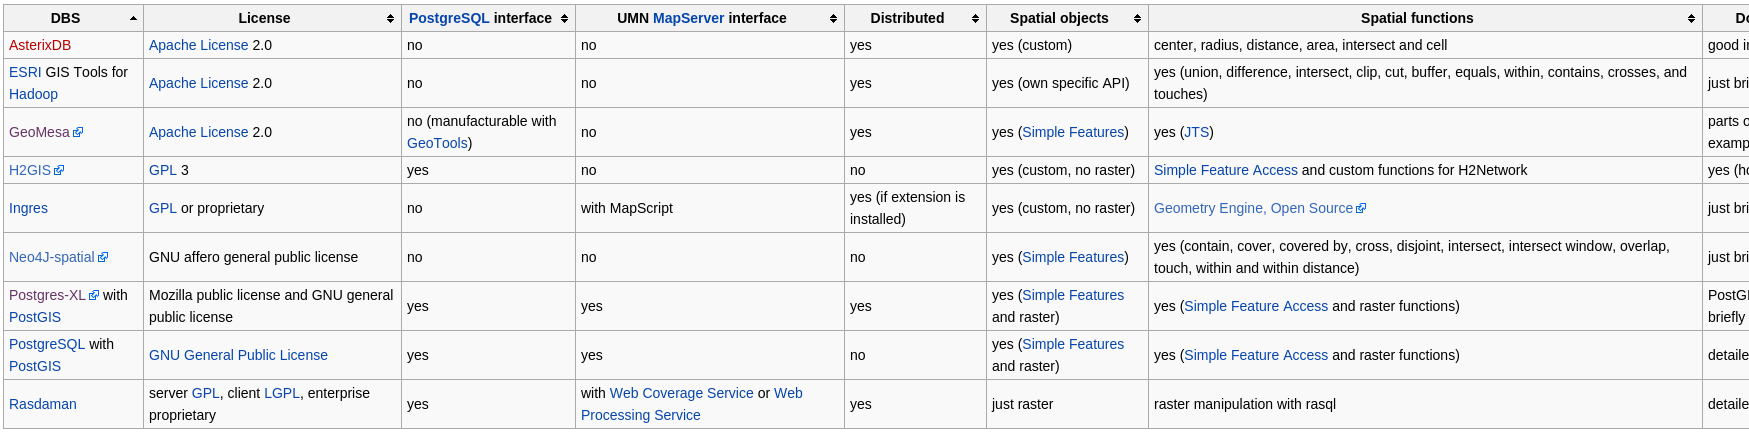
\includegraphics[height=.7\vsize]{spatial_databases3.png}
\caption{Relevante GIS nach Recherche}
\end{figure}
\begin{center}
\tiny
\url{https://en.wikipedia.org/wiki/Spatial_database}
\end{center}
%Auswahl nach Farbgebung
%Nutzwertanalyse mit Wichtung alle Metriken
\end{frame}

\begin{frame}\frametitle{Systemauswahl}

   \begin{columns}
    \begin{column}{.5\textwidth}
\ \ \ Nutzwert GeoMesa: 56
    \end{column}
    \begin{column}{.5\textwidth}
    
\includegraphics[width=.7\hsize]{geomesa.png}
    \end{column}
  \end{columns}
%https://raw.githubusercontent.com/geomesa/geomesa.github.io/master/img/geomesa-2x.png

\begin{table}
\begin{tabular}{|l|p{1.8cm}|l|p{1.9cm}|}
\hline
\textbf{Metrik} & \textbf{erreichter Wert} & \textbf{Erfüllung in \%} & \textbf{gewichteter Teilnutzen} \\ \hline
Interoperabilität & 7 & 58 & 17 \\ \hline
Funktionsumfang & 48 & 79 & 16 \\ \hline
Dokumentation & 4 & 31 & 11 \\ \hline
Modifizierbarkeit & 4 & 80 & 12 \\ \hline
\end{tabular}
\caption{Nutzwertanalyse GeoMesa}
\end{table}

\begin{center}
\tiny
\url{https://raw.githubusercontent.com/geomesa/geomesa.github.io/master/img/geomesa-2x.png}
\end{center}

\end{frame}

\begin{frame}\frametitle{Systemauswahl}

   \begin{columns}
    \begin{column}{.5\textwidth}
\ \ \ Nutzwert Postgres-XL: 86
    \end{column}
    \begin{column}{.5\textwidth}
    
\includegraphics[width=.45\hsize]{postgresxl.jpg}
    \end{column}
  \end{columns}
%http://www.postgres-xl.org/wp-content/uploads/2014/04/xl592x497g.jpg

\begin{table}
\begin{tabular}{|l|p{1.8cm}|l|p{1.9cm}|}
\hline
\textbf{Metrik} & \textbf{erreichter Wert} & \textbf{Erfüllung in \%} & \textbf{gewichteter Teilnutzen} \\ \hline
Interoperabilität & 12 & 100 & 30 \\ \hline
Funktionsumfang & 53 & 87 & 17 \\ \hline
Dokumentation & 9 & 69 & 24 \\ \hline
Modifizierbarkeit & 5 & 100 & 15 \\ \hline
\end{tabular}
\caption{Nutzwertanalyse Postgres-XL}
\end{table}

\begin{center}
\tiny
\url{http://www.postgres-xl.org/wp-content/uploads/2014/04/xl592x497g.jpg}
\end{center}
%Cluster DBMS

\end{frame}

\begin{frame}\frametitle{Systemauswahl}

   \begin{columns}
    \begin{column}{.5\textwidth}
\ \ \ Nutzwert Rasdaman: 51
    \end{column}
    \begin{column}{.5\textwidth}
    
\includegraphics[width=.6\hsize]{rasdaman.png}
    \end{column}
  \end{columns}
%http://www.faculty.jacobs-university.de/pbaumann/iu-bremen.de_pbaumann/Courses/InformationArchitecture/Rasdaman-doc/html/rasj/rasj/logo-rasdaman.gif

\begin{table}
\begin{tabular}{|l|p{1.8cm}|l|p{1.9cm}|}
\hline
\textbf{Metrik} & \textbf{erreichter Wert} & \textbf{Erfüllung in \%} & \textbf{gewichteter Teilnutzen} \\ \hline
Interoperabilität & 7 & 58 & 17 \\ \hline
Funktionsumfang & 10 & 16 & 3 \\ \hline
Dokumentation & 8 & 62 & 22 \\ \hline
Modifizierbarkeit & 3 & 60 & 9 \\ \hline
\end{tabular}
\caption{Nutzwertanalyse Rasdaman}
\end{table}

\begin{center}
\tiny
\url{http://www.rasdaman.org/chrome/site/trac_logo.png}
\end{center}

\end{frame}

\section{Untersuchung von Postgres-XL}
%Ausschnitt aus Thesis

%
\begin{frame}\frametitle{Untersuchung von Postgres-XL}

\begin{figure}
\centering
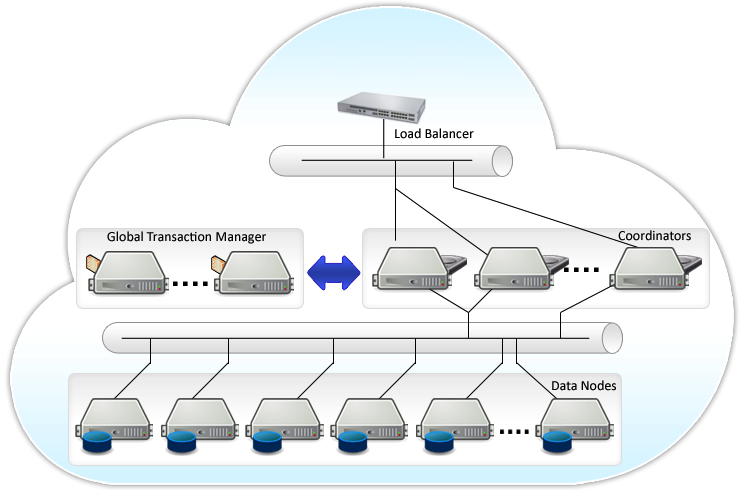
\includegraphics[width=1\hsize]{../Abbildungen/postgresxl-structure.jpg}
\caption{Aufbau von Postgres-XL}
\end{figure}
\end{frame}

\begin{frame}\frametitle{Untersuchung von Postgres-XL}
%Installation, Einrichtung
\begin{block}{Schnittstellen:}
Zugriff erfolgt analog zu PostgreSQL mit PostGIS über Coordinators.
%Für SQL und UMN
\end{block}

\vspace{\baselineskip}
\vspace{\baselineskip}

\begin{block}{Verarbeitung:}
Aufruf und Bibliotheken analog zu PostgreSQL mit PostGIS.\\
Abhängig von der Verteilung der Daten sind ausgewählte Knoten aktiv.
\end{block}

\end{frame}

\begin{frame}\frametitle{Untersuchung von Postgres-XL}
\begin{block}{Entwurf:}
Ähnlichkeit zu Ist-Stand bedingt Übernahme von Funktionalität.
\end{block}
% Fehlende Funktionalität wie Trigger und Problematik der verteilten Primärschlüssel bedingen Unmöglichkeit der kurzfristigen Realisierung
% Entwurf ist Clon des ISt-Standes ohne Trigger und angepasste FUnktionen/Schlüssel

\begin{figure}
\centering
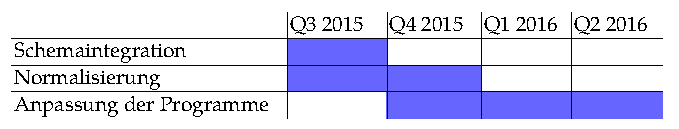
\includegraphics[width=1\hsize]{../Abbildungen/gantt_aufwand_umsetzung_cropped.pdf}
\caption{Aufwandsschätzung der teilweisen Integration}
\end{figure}
\end{frame}

\section{Tests}
%Ausschnitt aus Thesis

\begin{frame}\frametitle{Tests}
\centering\textbf{Testumgebung}

   \begin{columns}
    \begin{column}{.5\textwidth}
% Graphic for TeX using PGF
% Title: /home/tboonx/Dokumente/Studium/Masterarbeit/masterthesis/Abbildungen/Testsystem_physischerAufbau.dia
% Creator: Dia v0.97.2
% CreationDate: Sun Mar 22 16:47:12 2015
% For: tboonx
% \usepackage{tikz}
% The following commands are not supported in PSTricks at present
% We define them conditionally, so when they are implemented,
% this pgf file will use them.
\ifx\du\undefined
  \newlength{\du}
\fi
\setlength{\du}{15\unitlength}
\begin{tikzpicture}
\pgftransformxscale{1.000000}
\pgftransformyscale{-1.000000}
\definecolor{dialinecolor}{rgb}{0.000000, 0.000000, 0.000000}
\pgfsetstrokecolor{dialinecolor}
\definecolor{dialinecolor}{rgb}{1.000000, 1.000000, 1.000000}
\pgfsetfillcolor{dialinecolor}
\pgfsetlinewidth{0.100000\du}
\pgfsetdash{}{0pt}
\pgfsetdash{}{0pt}
\pgfsetbuttcap
\pgfsetmiterjoin
\pgfsetlinewidth{0.100000\du}
\pgfsetbuttcap
\pgfsetmiterjoin
\pgfsetdash{}{0pt}
\definecolor{dialinecolor}{rgb}{0.000000, 0.000000, 0.000000}
\pgfsetstrokecolor{dialinecolor}
\draw (38.088600\du,26.070243\du)--(38.088600\du,30.624686\du)--(39.606748\du,30.624686\du)--(39.606748\du,26.070243\du)--cycle;
\pgfsetlinewidth{0.010000\du}
\pgfsetbuttcap
\pgfsetmiterjoin
\pgfsetdash{}{0pt}
\definecolor{dialinecolor}{rgb}{0.000000, 0.000000, 0.000000}
\pgfsetstrokecolor{dialinecolor}
\draw (38.088600\du,26.070243\du)--(38.088600\du,30.624686\du)--(39.606748\du,30.624686\du)--(39.606748\du,26.070243\du)--cycle;
\pgfsetlinewidth{0.100000\du}
\pgfsetbuttcap
\pgfsetmiterjoin
\pgfsetdash{}{0pt}
\definecolor{dialinecolor}{rgb}{0.000000, 0.000000, 0.000000}
\pgfsetstrokecolor{dialinecolor}
\draw (38.240415\du,26.222058\du)--(38.240415\du,28.043835\du)--(39.454933\du,28.043835\du)--(39.454933\du,26.222058\du)--cycle;
\pgfsetlinewidth{0.010000\du}
\pgfsetbuttcap
\pgfsetmiterjoin
\pgfsetdash{}{0pt}
\definecolor{dialinecolor}{rgb}{0.000000, 0.000000, 0.000000}
\pgfsetstrokecolor{dialinecolor}
\draw (38.240415\du,26.222058\du)--(38.240415\du,28.043835\du)--(39.454933\du,28.043835\du)--(39.454933\du,26.222058\du)--cycle;
\pgfsetbuttcap
\pgfsetmiterjoin
\pgfsetdash{}{0pt}
\definecolor{dialinecolor}{rgb}{0.000000, 0.000000, 0.000000}
\pgfsetstrokecolor{dialinecolor}
\draw (38.240415\du,26.525688\du)--(39.454933\du,26.525688\du);
\pgfsetbuttcap
\pgfsetmiterjoin
\pgfsetdash{}{0pt}
\definecolor{dialinecolor}{rgb}{0.000000, 0.000000, 0.000000}
\pgfsetstrokecolor{dialinecolor}
\draw (39.454933\du,26.829317\du)--(38.240415\du,26.829317\du);
\pgfsetbuttcap
\pgfsetmiterjoin
\pgfsetdash{}{0pt}
\definecolor{dialinecolor}{rgb}{0.000000, 0.000000, 0.000000}
\pgfsetstrokecolor{dialinecolor}
\draw (38.240415\du,27.132947\du)--(39.454933\du,27.132947\du);
\pgfsetbuttcap
\pgfsetmiterjoin
\pgfsetdash{}{0pt}
\definecolor{dialinecolor}{rgb}{0.000000, 0.000000, 0.000000}
\pgfsetstrokecolor{dialinecolor}
\draw (38.240415\du,27.436576\du)--(39.454933\du,27.436576\du);
\pgfsetbuttcap
\pgfsetmiterjoin
\pgfsetdash{}{0pt}
\definecolor{dialinecolor}{rgb}{0.000000, 0.000000, 0.000000}
\pgfsetstrokecolor{dialinecolor}
\draw (39.454933\du,27.740206\du)--(38.240415\du,27.740206\du);
\pgfsetlinewidth{0.100000\du}
\pgfsetbuttcap
\pgfsetmiterjoin
\pgfsetdash{}{0pt}
\definecolor{dialinecolor}{rgb}{0.000000, 0.000000, 0.000000}
\pgfsetstrokecolor{dialinecolor}
\draw (38.240415\du,28.195650\du)--(38.240415\du,28.651094\du)--(39.075396\du,28.651094\du)--(39.075396\du,28.195650\du)--cycle;
\pgfsetlinewidth{0.010000\du}
\pgfsetbuttcap
\pgfsetmiterjoin
\pgfsetdash{}{0pt}
\definecolor{dialinecolor}{rgb}{0.000000, 0.000000, 0.000000}
\pgfsetstrokecolor{dialinecolor}
\draw (38.240415\du,28.195650\du)--(38.240415\du,28.651094\du)--(39.075396\du,28.651094\du)--(39.075396\du,28.195650\du)--cycle;
\pgfsetbuttcap
\pgfsetmiterjoin
\pgfsetdash{}{0pt}
\definecolor{dialinecolor}{rgb}{0.000000, 0.000000, 0.000000}
\pgfsetstrokecolor{dialinecolor}
\draw (38.088600\du,28.954724\du)--(39.606748\du,28.954724\du);
\pgfsetlinewidth{0.100000\du}
\pgfsetbuttcap
\pgfsetmiterjoin
\pgfsetdash{}{0pt}
\definecolor{dialinecolor}{rgb}{0.000000, 0.000000, 0.000000}
\pgfsetstrokecolor{dialinecolor}
\draw (38.771766\du,29.106539\du)--(38.771766\du,29.182446\du)--(38.847674\du,29.182446\du)--(38.847674\du,29.106539\du)--cycle;
\pgfsetlinewidth{0.010000\du}
\pgfsetbuttcap
\pgfsetmiterjoin
\pgfsetdash{}{0pt}
\definecolor{dialinecolor}{rgb}{0.000000, 0.000000, 0.000000}
\pgfsetstrokecolor{dialinecolor}
\draw (38.771766\du,29.106539\du)--(38.771766\du,29.182446\du)--(38.847674\du,29.182446\du)--(38.847674\du,29.106539\du)--cycle;
\pgfsetlinewidth{0.100000\du}
\pgfsetbuttcap
\pgfsetmiterjoin
\pgfsetdash{}{0pt}
\definecolor{dialinecolor}{rgb}{0.000000, 0.000000, 0.000000}
\pgfsetstrokecolor{dialinecolor}
\draw (39.075396\du,29.106539\du)--(39.075396\du,29.182446\du)--(39.151303\du,29.182446\du)--(39.151303\du,29.106539\du)--cycle;
\pgfsetlinewidth{0.010000\du}
\pgfsetbuttcap
\pgfsetmiterjoin
\pgfsetdash{}{0pt}
\definecolor{dialinecolor}{rgb}{0.000000, 0.000000, 0.000000}
\pgfsetstrokecolor{dialinecolor}
\draw (39.075396\du,29.106539\du)--(39.075396\du,29.182446\du)--(39.151303\du,29.182446\du)--(39.151303\du,29.106539\du)--cycle;
\pgfsetlinewidth{0.100000\du}
\pgfsetbuttcap
\pgfsetmiterjoin
\pgfsetdash{}{0pt}
\definecolor{dialinecolor}{rgb}{0.000000, 0.000000, 0.000000}
\pgfsetstrokecolor{dialinecolor}
\draw (39.379026\du,29.106539\du)--(39.379026\du,29.182446\du)--(39.454933\du,29.182446\du)--(39.454933\du,29.106539\du)--cycle;
\pgfsetlinewidth{0.010000\du}
\pgfsetbuttcap
\pgfsetmiterjoin
\pgfsetdash{}{0pt}
\definecolor{dialinecolor}{rgb}{0.000000, 0.000000, 0.000000}
\pgfsetstrokecolor{dialinecolor}
\draw (39.379026\du,29.106539\du)--(39.379026\du,29.182446\du)--(39.454933\du,29.182446\du)--(39.454933\du,29.106539\du)--cycle;
\pgfsetlinewidth{0.100000\du}
\pgfsetbuttcap
\pgfsetmiterjoin
\pgfsetdash{}{0pt}
\definecolor{dialinecolor}{rgb}{0.000000, 0.000000, 0.000000}
\pgfsetstrokecolor{dialinecolor}
\draw (39.303118\du,28.651094\du)--(39.303118\du,28.802909\du)--(39.454933\du,28.802909\du)--(39.454933\du,28.651094\du)--cycle;
\pgfsetlinewidth{0.010000\du}
\pgfsetbuttcap
\pgfsetmiterjoin
\pgfsetdash{}{0pt}
\definecolor{dialinecolor}{rgb}{0.000000, 0.000000, 0.000000}
\pgfsetstrokecolor{dialinecolor}
\draw (39.303118\du,28.651094\du)--(39.303118\du,28.802909\du)--(39.454933\du,28.802909\du)--(39.454933\du,28.651094\du)--cycle;
\pgfsetbuttcap
\pgfsetmiterjoin
\pgfsetdash{}{0pt}
\definecolor{dialinecolor}{rgb}{0.000000, 0.000000, 0.000000}
\pgfsetstrokecolor{dialinecolor}
\draw (38.240415\du,28.423372\du)--(39.075396\du,28.423372\du);
\pgfsetlinewidth{0.100000\du}
\pgfsetbuttcap
\pgfsetmiterjoin
\pgfsetdash{}{0pt}
\definecolor{dialinecolor}{rgb}{0.000000, 0.000000, 0.000000}
\pgfsetstrokecolor{dialinecolor}
\draw (38.240415\du,29.030631\du)--(38.240415\du,29.258353\du)--(38.468137\du,29.258353\du)--(38.468137\du,29.030631\du)--cycle;
\pgfsetlinewidth{0.010000\du}
\pgfsetbuttcap
\pgfsetmiterjoin
\pgfsetdash{}{0pt}
\definecolor{dialinecolor}{rgb}{0.000000, 0.000000, 0.000000}
\pgfsetstrokecolor{dialinecolor}
\draw (38.240415\du,29.030631\du)--(38.240415\du,29.258353\du)--(38.468137\du,29.258353\du)--(38.468137\du,29.030631\du)--cycle;
\pgfsetlinewidth{0.100000\du}
\pgfsetbuttcap
\pgfsetmiterjoin
\pgfsetdash{}{0pt}
\definecolor{dialinecolor}{rgb}{0.000000, 0.000000, 0.000000}
\pgfsetstrokecolor{dialinecolor}
\draw (38.316322\du,27.816113\du)--(38.316322\du,27.892021\du)--(39.379026\du,27.892021\du)--(39.379026\du,27.816113\du)--cycle;
\pgfsetlinewidth{0.010000\du}
\pgfsetbuttcap
\pgfsetmiterjoin
\pgfsetdash{}{0pt}
\definecolor{dialinecolor}{rgb}{0.000000, 0.000000, 0.000000}
\pgfsetstrokecolor{dialinecolor}
\draw (38.316322\du,27.816113\du)--(38.316322\du,27.892021\du)--(39.379026\du,27.892021\du)--(39.379026\du,27.816113\du)--cycle;
\pgfsetbuttcap
\pgfsetmiterjoin
\pgfsetdash{}{0pt}
\definecolor{dialinecolor}{rgb}{0.000000, 0.000000, 0.000000}
\pgfsetstrokecolor{dialinecolor}
\draw (38.316322\du,28.271557\du)--(38.999489\du,28.271557\du);
\pgfsetbuttcap
\pgfsetmiterjoin
\pgfsetdash{}{0pt}
\definecolor{dialinecolor}{rgb}{0.000000, 0.000000, 0.000000}
\pgfsetstrokecolor{dialinecolor}
\draw (38.999489\du,28.347465\du)--(38.923581\du,28.347465\du);
\pgfsetbuttcap
\pgfsetmiterjoin
\pgfsetdash{}{0pt}
\definecolor{dialinecolor}{rgb}{0.000000, 0.000000, 0.000000}
\pgfsetstrokecolor{dialinecolor}
\draw (38.316322\du,28.347465\du)--(38.392230\du,28.347465\du);
\pgfsetlinewidth{0.100000\du}
\pgfsetbuttcap
\pgfsetmiterjoin
\pgfsetdash{}{0pt}
\definecolor{dialinecolor}{rgb}{0.000000, 0.000000, 0.000000}
\pgfsetstrokecolor{dialinecolor}
\draw (38.468137\du,28.271557\du)--(38.468137\du,28.347465\du)--(38.847674\du,28.347465\du)--(38.847674\du,28.271557\du)--cycle;
\pgfsetlinewidth{0.010000\du}
\pgfsetbuttcap
\pgfsetmiterjoin
\pgfsetdash{}{0pt}
\definecolor{dialinecolor}{rgb}{0.000000, 0.000000, 0.000000}
\pgfsetstrokecolor{dialinecolor}
\draw (38.468137\du,28.271557\du)--(38.468137\du,28.347465\du)--(38.847674\du,28.347465\du)--(38.847674\du,28.271557\du)--cycle;
\pgfsetbuttcap
\pgfsetmiterjoin
\pgfsetdash{}{0pt}
\definecolor{dialinecolor}{rgb}{0.000000, 0.000000, 0.000000}
\pgfsetstrokecolor{dialinecolor}
\draw (38.316322\du,27.967928\du)--(38.392230\du,27.967928\du);
\pgfsetbuttcap
\pgfsetmiterjoin
\pgfsetdash{}{0pt}
\definecolor{dialinecolor}{rgb}{0.000000, 0.000000, 0.000000}
\pgfsetstrokecolor{dialinecolor}
\draw (38.468137\du,27.967928\du)--(38.544044\du,27.967928\du);
\pgfsetbuttcap
\pgfsetmiterjoin
\pgfsetdash{}{0pt}
\definecolor{dialinecolor}{rgb}{0.000000, 0.000000, 0.000000}
\pgfsetstrokecolor{dialinecolor}
\draw (39.227211\du,27.967928\du)--(39.379026\du,27.967928\du);
\pgfsetbuttcap
\pgfsetmiterjoin
\pgfsetdash{}{0pt}
\definecolor{dialinecolor}{rgb}{0.000000, 0.000000, 0.000000}
\pgfsetstrokecolor{dialinecolor}
\draw (38.164507\du,30.548779\du)--(39.530840\du,30.548779\du);
\pgfsetbuttcap
\pgfsetmiterjoin
\pgfsetdash{}{0pt}
\definecolor{dialinecolor}{rgb}{0.000000, 0.000000, 0.000000}
\pgfsetstrokecolor{dialinecolor}
\draw (39.530840\du,30.472872\du)--(38.164507\du,30.472872\du);
\pgfsetbuttcap
\pgfsetmiterjoin
\pgfsetdash{}{0pt}
\definecolor{dialinecolor}{rgb}{0.000000, 0.000000, 0.000000}
\pgfsetstrokecolor{dialinecolor}
\draw (38.164507\du,30.396964\du)--(39.530840\du,30.396964\du);
\pgfsetbuttcap
\pgfsetmiterjoin
\pgfsetdash{}{0pt}
\definecolor{dialinecolor}{rgb}{0.000000, 0.000000, 0.000000}
\pgfsetstrokecolor{dialinecolor}
\draw (39.530840\du,30.321057\du)--(38.164507\du,30.321057\du);
\pgfsetbuttcap
\pgfsetmiterjoin
\pgfsetdash{}{0pt}
\definecolor{dialinecolor}{rgb}{0.000000, 0.000000, 0.000000}
\pgfsetstrokecolor{dialinecolor}
\draw (38.164507\du,30.245150\du)--(39.530840\du,30.245150\du);
\pgfsetbuttcap
\pgfsetmiterjoin
\pgfsetdash{}{0pt}
\definecolor{dialinecolor}{rgb}{0.000000, 0.000000, 0.000000}
\pgfsetstrokecolor{dialinecolor}
\draw (39.530840\du,30.169242\du)--(38.164507\du,30.169242\du);
\pgfsetbuttcap
\pgfsetmiterjoin
\pgfsetdash{}{0pt}
\definecolor{dialinecolor}{rgb}{0.000000, 0.000000, 0.000000}
\pgfsetstrokecolor{dialinecolor}
\draw (38.164507\du,30.093335\du)--(39.530840\du,30.093335\du);
\pgfsetbuttcap
\pgfsetmiterjoin
\pgfsetdash{}{0pt}
\definecolor{dialinecolor}{rgb}{0.000000, 0.000000, 0.000000}
\pgfsetstrokecolor{dialinecolor}
\draw (39.530840\du,30.017427\du)--(38.164507\du,30.017427\du);
\pgfsetbuttcap
\pgfsetmiterjoin
\pgfsetdash{}{0pt}
\definecolor{dialinecolor}{rgb}{0.000000, 0.000000, 0.000000}
\pgfsetstrokecolor{dialinecolor}
\draw (38.164507\du,29.941520\du)--(39.530840\du,29.941520\du);
\pgfsetbuttcap
\pgfsetmiterjoin
\pgfsetdash{}{0pt}
\definecolor{dialinecolor}{rgb}{0.000000, 0.000000, 0.000000}
\pgfsetstrokecolor{dialinecolor}
\draw (39.530840\du,29.865613\du)--(38.164507\du,29.865613\du);
\pgfsetbuttcap
\pgfsetmiterjoin
\pgfsetdash{}{0pt}
\definecolor{dialinecolor}{rgb}{0.000000, 0.000000, 0.000000}
\pgfsetstrokecolor{dialinecolor}
\draw (38.164507\du,29.789705\du)--(39.530840\du,29.789705\du);
\pgfsetbuttcap
\pgfsetmiterjoin
\pgfsetdash{}{0pt}
\definecolor{dialinecolor}{rgb}{0.000000, 0.000000, 0.000000}
\pgfsetstrokecolor{dialinecolor}
\draw (39.530840\du,29.713798\du)--(38.164507\du,29.713798\du);
\pgfsetbuttcap
\pgfsetmiterjoin
\pgfsetdash{}{0pt}
\definecolor{dialinecolor}{rgb}{0.000000, 0.000000, 0.000000}
\pgfsetstrokecolor{dialinecolor}
\draw (38.164507\du,29.637890\du)--(39.530840\du,29.637890\du);
\pgfsetbuttcap
\pgfsetmiterjoin
\pgfsetdash{}{0pt}
\definecolor{dialinecolor}{rgb}{0.000000, 0.000000, 0.000000}
\pgfsetstrokecolor{dialinecolor}
\draw (39.530840\du,29.561983\du)--(38.164507\du,29.561983\du);
% setfont left to latex
\definecolor{dialinecolor}{rgb}{0.000000, 0.000000, 0.000000}
\pgfsetstrokecolor{dialinecolor}
\node at (38.636700\du,24.819100\du){VMware vCenter Server};
% setfont left to latex
\definecolor{dialinecolor}{rgb}{0.000000, 0.000000, 0.000000}
\pgfsetstrokecolor{dialinecolor}
\node at (38.636700\du,25.619100\du){VMware vSphere Client};
\pgfsetlinewidth{0.100000\du}
\pgfsetdash{}{0pt}
\pgfsetdash{}{0pt}
\pgfsetbuttcap
\pgfsetmiterjoin
\pgfsetlinewidth{0.100000\du}
\pgfsetbuttcap
\pgfsetmiterjoin
\pgfsetdash{}{0pt}
\definecolor{dialinecolor}{rgb}{0.000000, 0.000000, 0.000000}
\pgfsetstrokecolor{dialinecolor}
\draw (35.650000\du,34.105300\du)--(35.650000\du,35.713097\du)--(42.081186\du,35.713097\du)--(42.081186\du,34.105300\du)--cycle;
\pgfsetlinewidth{0.010000\du}
\pgfsetbuttcap
\pgfsetmiterjoin
\pgfsetdash{}{0pt}
\definecolor{dialinecolor}{rgb}{0.000000, 0.000000, 0.000000}
\pgfsetstrokecolor{dialinecolor}
\draw (35.650000\du,34.105300\du)--(35.650000\du,35.713097\du)--(42.081186\du,35.713097\du)--(42.081186\du,34.105300\du)--cycle;
\pgfsetbuttcap
\pgfsetmiterjoin
\pgfsetdash{}{0pt}
\definecolor{dialinecolor}{rgb}{0.000000, 0.000000, 0.000000}
\pgfsetstrokecolor{dialinecolor}
\draw (36.775458\du,34.748419\du)--(36.614678\du,34.909198\du);
\pgfsetbuttcap
\pgfsetmiterjoin
\pgfsetdash{}{0pt}
\definecolor{dialinecolor}{rgb}{0.000000, 0.000000, 0.000000}
\pgfsetstrokecolor{dialinecolor}
\draw (36.614678\du,34.909198\du)--(36.775458\du,35.069978\du);
\pgfsetbuttcap
\pgfsetmiterjoin
\pgfsetdash{}{0pt}
\definecolor{dialinecolor}{rgb}{0.000000, 0.000000, 0.000000}
\pgfsetstrokecolor{dialinecolor}
\draw (37.418576\du,34.748419\du)--(37.257797\du,34.909198\du);
\pgfsetbuttcap
\pgfsetmiterjoin
\pgfsetdash{}{0pt}
\definecolor{dialinecolor}{rgb}{0.000000, 0.000000, 0.000000}
\pgfsetstrokecolor{dialinecolor}
\draw (37.257797\du,34.909198\du)--(37.418576\du,35.069978\du);
\pgfsetbuttcap
\pgfsetmiterjoin
\pgfsetdash{}{0pt}
\definecolor{dialinecolor}{rgb}{0.000000, 0.000000, 0.000000}
\pgfsetstrokecolor{dialinecolor}
\draw (38.061695\du,34.748419\du)--(37.900915\du,34.909198\du);
\pgfsetbuttcap
\pgfsetmiterjoin
\pgfsetdash{}{0pt}
\definecolor{dialinecolor}{rgb}{0.000000, 0.000000, 0.000000}
\pgfsetstrokecolor{dialinecolor}
\draw (37.900915\du,34.909198\du)--(38.061695\du,35.069978\du);
\pgfsetbuttcap
\pgfsetmiterjoin
\pgfsetdash{}{0pt}
\definecolor{dialinecolor}{rgb}{0.000000, 0.000000, 0.000000}
\pgfsetstrokecolor{dialinecolor}
\draw (38.704814\du,34.748419\du)--(38.544034\du,34.909198\du);
\pgfsetbuttcap
\pgfsetmiterjoin
\pgfsetdash{}{0pt}
\definecolor{dialinecolor}{rgb}{0.000000, 0.000000, 0.000000}
\pgfsetstrokecolor{dialinecolor}
\draw (38.544034\du,34.909198\du)--(38.704814\du,35.069978\du);
\pgfsetbuttcap
\pgfsetmiterjoin
\pgfsetdash{}{0pt}
\definecolor{dialinecolor}{rgb}{0.000000, 0.000000, 0.000000}
\pgfsetstrokecolor{dialinecolor}
\draw (39.347932\du,34.748419\du)--(39.187153\du,34.909198\du);
\pgfsetbuttcap
\pgfsetmiterjoin
\pgfsetdash{}{0pt}
\definecolor{dialinecolor}{rgb}{0.000000, 0.000000, 0.000000}
\pgfsetstrokecolor{dialinecolor}
\draw (39.187153\du,34.909198\du)--(39.347932\du,35.069978\du);
\pgfsetbuttcap
\pgfsetmiterjoin
\pgfsetdash{}{0pt}
\definecolor{dialinecolor}{rgb}{0.000000, 0.000000, 0.000000}
\pgfsetstrokecolor{dialinecolor}
\draw (39.991051\du,34.748419\du)--(39.830271\du,34.909198\du);
\pgfsetbuttcap
\pgfsetmiterjoin
\pgfsetdash{}{0pt}
\definecolor{dialinecolor}{rgb}{0.000000, 0.000000, 0.000000}
\pgfsetstrokecolor{dialinecolor}
\draw (39.830271\du,34.909198\du)--(39.991051\du,35.069978\du);
\pgfsetbuttcap
\pgfsetmiterjoin
\pgfsetdash{}{0pt}
\definecolor{dialinecolor}{rgb}{0.000000, 0.000000, 0.000000}
\pgfsetstrokecolor{dialinecolor}
\draw (40.634170\du,34.748419\du)--(40.473390\du,34.909198\du);
\pgfsetbuttcap
\pgfsetmiterjoin
\pgfsetdash{}{0pt}
\definecolor{dialinecolor}{rgb}{0.000000, 0.000000, 0.000000}
\pgfsetstrokecolor{dialinecolor}
\draw (40.473390\du,34.909198\du)--(40.634170\du,35.069978\du);
\pgfsetbuttcap
\pgfsetmiterjoin
\pgfsetdash{}{0pt}
\definecolor{dialinecolor}{rgb}{0.000000, 0.000000, 0.000000}
\pgfsetstrokecolor{dialinecolor}
\draw (41.277288\du,34.748419\du)--(41.116509\du,34.909198\du);
\pgfsetbuttcap
\pgfsetmiterjoin
\pgfsetdash{}{0pt}
\definecolor{dialinecolor}{rgb}{0.000000, 0.000000, 0.000000}
\pgfsetstrokecolor{dialinecolor}
\draw (41.116509\du,34.909198\du)--(41.277288\du,35.069978\du);
\pgfsetbuttcap
\pgfsetmiterjoin
\pgfsetdash{}{0pt}
\definecolor{dialinecolor}{rgb}{0.000000, 0.000000, 0.000000}
\pgfsetstrokecolor{dialinecolor}
\draw (41.598847\du,35.230758\du)--(41.438068\du,35.391537\du);
\pgfsetbuttcap
\pgfsetmiterjoin
\pgfsetdash{}{0pt}
\definecolor{dialinecolor}{rgb}{0.000000, 0.000000, 0.000000}
\pgfsetstrokecolor{dialinecolor}
\draw (41.438068\du,35.391537\du)--(41.598847\du,35.552317\du);
\pgfsetbuttcap
\pgfsetmiterjoin
\pgfsetdash{}{0pt}
\definecolor{dialinecolor}{rgb}{0.000000, 0.000000, 0.000000}
\pgfsetstrokecolor{dialinecolor}
\draw (40.955729\du,35.230758\du)--(40.794949\du,35.391537\du);
\pgfsetbuttcap
\pgfsetmiterjoin
\pgfsetdash{}{0pt}
\definecolor{dialinecolor}{rgb}{0.000000, 0.000000, 0.000000}
\pgfsetstrokecolor{dialinecolor}
\draw (40.794949\du,35.391537\du)--(40.955729\du,35.552317\du);
\pgfsetbuttcap
\pgfsetmiterjoin
\pgfsetdash{}{0pt}
\definecolor{dialinecolor}{rgb}{0.000000, 0.000000, 0.000000}
\pgfsetstrokecolor{dialinecolor}
\draw (40.312610\du,35.230758\du)--(40.151831\du,35.391537\du);
\pgfsetbuttcap
\pgfsetmiterjoin
\pgfsetdash{}{0pt}
\definecolor{dialinecolor}{rgb}{0.000000, 0.000000, 0.000000}
\pgfsetstrokecolor{dialinecolor}
\draw (40.151831\du,35.391537\du)--(40.312610\du,35.552317\du);
\pgfsetbuttcap
\pgfsetmiterjoin
\pgfsetdash{}{0pt}
\definecolor{dialinecolor}{rgb}{0.000000, 0.000000, 0.000000}
\pgfsetstrokecolor{dialinecolor}
\draw (39.669492\du,35.230758\du)--(39.508712\du,35.391537\du);
\pgfsetbuttcap
\pgfsetmiterjoin
\pgfsetdash{}{0pt}
\definecolor{dialinecolor}{rgb}{0.000000, 0.000000, 0.000000}
\pgfsetstrokecolor{dialinecolor}
\draw (39.508712\du,35.391537\du)--(39.669492\du,35.552317\du);
\pgfsetbuttcap
\pgfsetmiterjoin
\pgfsetdash{}{0pt}
\definecolor{dialinecolor}{rgb}{0.000000, 0.000000, 0.000000}
\pgfsetstrokecolor{dialinecolor}
\draw (39.026373\du,35.230758\du)--(38.865593\du,35.391537\du);
\pgfsetbuttcap
\pgfsetmiterjoin
\pgfsetdash{}{0pt}
\definecolor{dialinecolor}{rgb}{0.000000, 0.000000, 0.000000}
\pgfsetstrokecolor{dialinecolor}
\draw (38.865593\du,35.391537\du)--(39.026373\du,35.552317\du);
\pgfsetbuttcap
\pgfsetmiterjoin
\pgfsetdash{}{0pt}
\definecolor{dialinecolor}{rgb}{0.000000, 0.000000, 0.000000}
\pgfsetstrokecolor{dialinecolor}
\draw (38.383254\du,35.230758\du)--(38.222475\du,35.391537\du);
\pgfsetbuttcap
\pgfsetmiterjoin
\pgfsetdash{}{0pt}
\definecolor{dialinecolor}{rgb}{0.000000, 0.000000, 0.000000}
\pgfsetstrokecolor{dialinecolor}
\draw (38.222475\du,35.391537\du)--(38.383254\du,35.552317\du);
\pgfsetbuttcap
\pgfsetmiterjoin
\pgfsetdash{}{0pt}
\definecolor{dialinecolor}{rgb}{0.000000, 0.000000, 0.000000}
\pgfsetstrokecolor{dialinecolor}
\draw (37.740136\du,35.230758\du)--(37.579356\du,35.391537\du);
\pgfsetbuttcap
\pgfsetmiterjoin
\pgfsetdash{}{0pt}
\definecolor{dialinecolor}{rgb}{0.000000, 0.000000, 0.000000}
\pgfsetstrokecolor{dialinecolor}
\draw (37.579356\du,35.391537\du)--(37.740136\du,35.552317\du);
\pgfsetlinewidth{0.100000\du}
\pgfsetbuttcap
\pgfsetmiterjoin
\pgfsetdash{}{0pt}
\definecolor{dialinecolor}{rgb}{0.000000, 0.000000, 0.000000}
\pgfsetstrokecolor{dialinecolor}
\draw (36.775458\du,35.391537\du)--(36.775458\du,35.552317\du)--(37.418576\du,35.552317\du)--(37.418576\du,35.391537\du)--cycle;
\pgfsetlinewidth{0.010000\du}
\pgfsetbuttcap
\pgfsetmiterjoin
\pgfsetdash{}{0pt}
\definecolor{dialinecolor}{rgb}{0.000000, 0.000000, 0.000000}
\pgfsetstrokecolor{dialinecolor}
\draw (36.775458\du,35.391537\du)--(36.775458\du,35.552317\du)--(37.418576\du,35.552317\du)--(37.418576\du,35.391537\du)--cycle;
\pgfsetlinewidth{0.100000\du}
\pgfsetbuttcap
\pgfsetmiterjoin
\pgfsetdash{}{0pt}
\definecolor{dialinecolor}{rgb}{0.000000, 0.000000, 0.000000}
\pgfsetstrokecolor{dialinecolor}
\draw (36.132339\du,34.909198\du)--(36.453898\du,35.230758\du)--(36.132339\du,35.552317\du)--(35.810780\du,35.230758\du)--cycle;
\pgfsetlinewidth{0.010000\du}
\pgfsetbuttcap
\pgfsetmiterjoin
\pgfsetdash{}{0pt}
\definecolor{dialinecolor}{rgb}{0.000000, 0.000000, 0.000000}
\pgfsetstrokecolor{dialinecolor}
\draw (36.132339\du,34.909198\du)--(36.453898\du,35.230758\du)--(36.132339\du,35.552317\du)--(35.810780\du,35.230758\du)--cycle;
\pgfsetlinewidth{0.100000\du}
\pgfsetbuttcap
\pgfsetmiterjoin
\pgfsetdash{}{0pt}
\definecolor{dialinecolor}{rgb}{0.000000, 0.000000, 0.000000}
\pgfsetstrokecolor{dialinecolor}
\draw (35.650000\du,34.426859\du)--(35.650000\du,34.587639\du)--(42.081186\du,34.587639\du)--(42.081186\du,34.426859\du)--cycle;
\pgfsetlinewidth{0.010000\du}
\pgfsetbuttcap
\pgfsetmiterjoin
\pgfsetdash{}{0pt}
\definecolor{dialinecolor}{rgb}{0.000000, 0.000000, 0.000000}
\pgfsetstrokecolor{dialinecolor}
\draw (35.650000\du,34.426859\du)--(35.650000\du,34.587639\du)--(42.081186\du,34.587639\du)--(42.081186\du,34.426859\du)--cycle;
\pgfsetlinewidth{0.100000\du}
\pgfsetbuttcap
\pgfsetmiterjoin
\pgfsetdash{}{0pt}
\definecolor{dialinecolor}{rgb}{0.000000, 0.000000, 0.000000}
\pgfsetstrokecolor{dialinecolor}
\draw (36.453898\du,34.426859\du)--(36.453898\du,34.587639\du)--(37.900915\du,34.587639\du)--(37.900915\du,34.426859\du)--cycle;
\pgfsetlinewidth{0.010000\du}
\pgfsetbuttcap
\pgfsetmiterjoin
\pgfsetdash{}{0pt}
\definecolor{dialinecolor}{rgb}{0.000000, 0.000000, 0.000000}
\pgfsetstrokecolor{dialinecolor}
\draw (36.453898\du,34.426859\du)--(36.453898\du,34.587639\du)--(37.900915\du,34.587639\du)--(37.900915\du,34.426859\du)--cycle;
% setfont left to latex
\definecolor{dialinecolor}{rgb}{0.000000, 0.000000, 0.000000}
\pgfsetstrokecolor{dialinecolor}
\node at (39.078800\du,36.378000\du){IBM RackServer};
% setfont left to latex
\definecolor{dialinecolor}{rgb}{0.000000, 0.000000, 0.000000}
\pgfsetstrokecolor{dialinecolor}
\node at (39.078800\du,37.178000\du){VMware ESXi};
\pgfsetlinewidth{0.100000\du}
\pgfsetdash{}{0pt}
\pgfsetdash{}{0pt}
\pgfsetbuttcap
{
\definecolor{dialinecolor}{rgb}{0.000000, 0.000000, 0.000000}
\pgfsetfillcolor{dialinecolor}
% was here!!!
\pgfsetarrowsstart{latex}
\pgfsetarrowsend{latex}
\definecolor{dialinecolor}{rgb}{0.000000, 0.000000, 0.000000}
\pgfsetstrokecolor{dialinecolor}
\draw (38.847674\du,30.624686\du)--(38.865593\du,34.105300\du);
}
% setfont left to latex
\definecolor{dialinecolor}{rgb}{0.000000, 0.000000, 0.000000}
\pgfsetstrokecolor{dialinecolor}
\node[anchor=west] at (38.959000\du,32.514900\du){Ethernet};
\end{tikzpicture}

    \end{column}
    \begin{column}{.5\textwidth}
\resizebox{1\linewidth}{!}{% Graphic for TeX using PGF
% Title: /home/tboonx/Dokumente/Studium/Masterarbeit/masterthesis/Abbildungen/Testsystem_VMs.dia
% Creator: Dia v0.97.2
% CreationDate: Thu Apr 23 17:29:28 2015
% For: tboonx
% \usepackage{tikz}
% The following commands are not supported in PSTricks at present
% We define them conditionally, so when they are implemented,
% this pgf file will use them.
\ifx\du\undefined
  \newlength{\du}
\fi
\setlength{\du}{15\unitlength}
\begin{tikzpicture}
\pgftransformxscale{1.000000}
\pgftransformyscale{-1.000000}
\definecolor{dialinecolor}{rgb}{0.000000, 0.000000, 0.000000}
\pgfsetstrokecolor{dialinecolor}
\definecolor{dialinecolor}{rgb}{1.000000, 1.000000, 1.000000}
\pgfsetfillcolor{dialinecolor}
\pgfsetlinewidth{0.100000\du}
\pgfsetdash{}{0pt}
\pgfsetdash{}{0pt}
\pgfsetmiterjoin
\pgfsetbuttcap
\definecolor{dialinecolor}{rgb}{0.000000, 0.000000, 0.000000}
\pgfsetstrokecolor{dialinecolor}
\draw (48.300000\du,24.162500\du)--(53.200000\du,24.212500\du)--(53.150000\du,26.712500\du)--(55.550000\du,26.762500\du)--(55.550000\du,35.162500\du)--(46.050000\du,35.112500\du)--(46.100000\du,26.862500\du)--(48.350000\du,26.862500\du)--cycle;
\pgfsetlinewidth{0.100000\du}
\pgfsetdash{}{0pt}
\pgfsetdash{}{0pt}
\pgfsetbuttcap
\pgfsetmiterjoin
\pgfsetlinewidth{0.100000\du}
\pgfsetbuttcap
\pgfsetmiterjoin
\pgfsetdash{}{0pt}
\definecolor{dialinecolor}{rgb}{0.000000, 0.000000, 0.000000}
\pgfsetstrokecolor{dialinecolor}
\draw (48.874800\du,24.869200\du)--(48.874800\du,25.775015\du)--(52.498061\du,25.775015\du)--(52.498061\du,24.869200\du)--cycle;
\pgfsetlinewidth{0.010000\du}
\pgfsetbuttcap
\pgfsetmiterjoin
\pgfsetdash{}{0pt}
\definecolor{dialinecolor}{rgb}{0.000000, 0.000000, 0.000000}
\pgfsetstrokecolor{dialinecolor}
\draw (48.874800\du,24.869200\du)--(48.874800\du,25.775015\du)--(52.498061\du,25.775015\du)--(52.498061\du,24.869200\du)--cycle;
\pgfsetbuttcap
\pgfsetmiterjoin
\pgfsetdash{}{0pt}
\definecolor{dialinecolor}{rgb}{0.000000, 0.000000, 0.000000}
\pgfsetstrokecolor{dialinecolor}
\draw (49.508871\du,25.231526\du)--(49.418289\du,25.322108\du);
\pgfsetbuttcap
\pgfsetmiterjoin
\pgfsetdash{}{0pt}
\definecolor{dialinecolor}{rgb}{0.000000, 0.000000, 0.000000}
\pgfsetstrokecolor{dialinecolor}
\draw (49.418289\du,25.322108\du)--(49.508871\du,25.412689\du);
\pgfsetbuttcap
\pgfsetmiterjoin
\pgfsetdash{}{0pt}
\definecolor{dialinecolor}{rgb}{0.000000, 0.000000, 0.000000}
\pgfsetstrokecolor{dialinecolor}
\draw (49.871197\du,25.231526\du)--(49.780615\du,25.322108\du);
\pgfsetbuttcap
\pgfsetmiterjoin
\pgfsetdash{}{0pt}
\definecolor{dialinecolor}{rgb}{0.000000, 0.000000, 0.000000}
\pgfsetstrokecolor{dialinecolor}
\draw (49.780615\du,25.322108\du)--(49.871197\du,25.412689\du);
\pgfsetbuttcap
\pgfsetmiterjoin
\pgfsetdash{}{0pt}
\definecolor{dialinecolor}{rgb}{0.000000, 0.000000, 0.000000}
\pgfsetstrokecolor{dialinecolor}
\draw (50.233523\du,25.231526\du)--(50.142941\du,25.322108\du);
\pgfsetbuttcap
\pgfsetmiterjoin
\pgfsetdash{}{0pt}
\definecolor{dialinecolor}{rgb}{0.000000, 0.000000, 0.000000}
\pgfsetstrokecolor{dialinecolor}
\draw (50.142941\du,25.322108\du)--(50.233523\du,25.412689\du);
\pgfsetbuttcap
\pgfsetmiterjoin
\pgfsetdash{}{0pt}
\definecolor{dialinecolor}{rgb}{0.000000, 0.000000, 0.000000}
\pgfsetstrokecolor{dialinecolor}
\draw (50.595849\du,25.231526\du)--(50.505268\du,25.322108\du);
\pgfsetbuttcap
\pgfsetmiterjoin
\pgfsetdash{}{0pt}
\definecolor{dialinecolor}{rgb}{0.000000, 0.000000, 0.000000}
\pgfsetstrokecolor{dialinecolor}
\draw (50.505268\du,25.322108\du)--(50.595849\du,25.412689\du);
\pgfsetbuttcap
\pgfsetmiterjoin
\pgfsetdash{}{0pt}
\definecolor{dialinecolor}{rgb}{0.000000, 0.000000, 0.000000}
\pgfsetstrokecolor{dialinecolor}
\draw (50.958175\du,25.231526\du)--(50.867594\du,25.322108\du);
\pgfsetbuttcap
\pgfsetmiterjoin
\pgfsetdash{}{0pt}
\definecolor{dialinecolor}{rgb}{0.000000, 0.000000, 0.000000}
\pgfsetstrokecolor{dialinecolor}
\draw (50.867594\du,25.322108\du)--(50.958175\du,25.412689\du);
\pgfsetbuttcap
\pgfsetmiterjoin
\pgfsetdash{}{0pt}
\definecolor{dialinecolor}{rgb}{0.000000, 0.000000, 0.000000}
\pgfsetstrokecolor{dialinecolor}
\draw (51.320501\du,25.231526\du)--(51.229920\du,25.322108\du);
\pgfsetbuttcap
\pgfsetmiterjoin
\pgfsetdash{}{0pt}
\definecolor{dialinecolor}{rgb}{0.000000, 0.000000, 0.000000}
\pgfsetstrokecolor{dialinecolor}
\draw (51.229920\du,25.322108\du)--(51.320501\du,25.412689\du);
\pgfsetbuttcap
\pgfsetmiterjoin
\pgfsetdash{}{0pt}
\definecolor{dialinecolor}{rgb}{0.000000, 0.000000, 0.000000}
\pgfsetstrokecolor{dialinecolor}
\draw (51.682827\du,25.231526\du)--(51.592246\du,25.322108\du);
\pgfsetbuttcap
\pgfsetmiterjoin
\pgfsetdash{}{0pt}
\definecolor{dialinecolor}{rgb}{0.000000, 0.000000, 0.000000}
\pgfsetstrokecolor{dialinecolor}
\draw (51.592246\du,25.322108\du)--(51.682827\du,25.412689\du);
\pgfsetbuttcap
\pgfsetmiterjoin
\pgfsetdash{}{0pt}
\definecolor{dialinecolor}{rgb}{0.000000, 0.000000, 0.000000}
\pgfsetstrokecolor{dialinecolor}
\draw (52.045154\du,25.231526\du)--(51.954572\du,25.322108\du);
\pgfsetbuttcap
\pgfsetmiterjoin
\pgfsetdash{}{0pt}
\definecolor{dialinecolor}{rgb}{0.000000, 0.000000, 0.000000}
\pgfsetstrokecolor{dialinecolor}
\draw (51.954572\du,25.322108\du)--(52.045154\du,25.412689\du);
\pgfsetbuttcap
\pgfsetmiterjoin
\pgfsetdash{}{0pt}
\definecolor{dialinecolor}{rgb}{0.000000, 0.000000, 0.000000}
\pgfsetstrokecolor{dialinecolor}
\draw (52.226317\du,25.503271\du)--(52.135735\du,25.593852\du);
\pgfsetbuttcap
\pgfsetmiterjoin
\pgfsetdash{}{0pt}
\definecolor{dialinecolor}{rgb}{0.000000, 0.000000, 0.000000}
\pgfsetstrokecolor{dialinecolor}
\draw (52.135735\du,25.593852\du)--(52.226317\du,25.684434\du);
\pgfsetbuttcap
\pgfsetmiterjoin
\pgfsetdash{}{0pt}
\definecolor{dialinecolor}{rgb}{0.000000, 0.000000, 0.000000}
\pgfsetstrokecolor{dialinecolor}
\draw (51.863990\du,25.503271\du)--(51.773409\du,25.593852\du);
\pgfsetbuttcap
\pgfsetmiterjoin
\pgfsetdash{}{0pt}
\definecolor{dialinecolor}{rgb}{0.000000, 0.000000, 0.000000}
\pgfsetstrokecolor{dialinecolor}
\draw (51.773409\du,25.593852\du)--(51.863990\du,25.684434\du);
\pgfsetbuttcap
\pgfsetmiterjoin
\pgfsetdash{}{0pt}
\definecolor{dialinecolor}{rgb}{0.000000, 0.000000, 0.000000}
\pgfsetstrokecolor{dialinecolor}
\draw (51.501664\du,25.503271\du)--(51.411083\du,25.593852\du);
\pgfsetbuttcap
\pgfsetmiterjoin
\pgfsetdash{}{0pt}
\definecolor{dialinecolor}{rgb}{0.000000, 0.000000, 0.000000}
\pgfsetstrokecolor{dialinecolor}
\draw (51.411083\du,25.593852\du)--(51.501664\du,25.684434\du);
\pgfsetbuttcap
\pgfsetmiterjoin
\pgfsetdash{}{0pt}
\definecolor{dialinecolor}{rgb}{0.000000, 0.000000, 0.000000}
\pgfsetstrokecolor{dialinecolor}
\draw (51.139338\du,25.503271\du)--(51.048757\du,25.593852\du);
\pgfsetbuttcap
\pgfsetmiterjoin
\pgfsetdash{}{0pt}
\definecolor{dialinecolor}{rgb}{0.000000, 0.000000, 0.000000}
\pgfsetstrokecolor{dialinecolor}
\draw (51.048757\du,25.593852\du)--(51.139338\du,25.684434\du);
\pgfsetbuttcap
\pgfsetmiterjoin
\pgfsetdash{}{0pt}
\definecolor{dialinecolor}{rgb}{0.000000, 0.000000, 0.000000}
\pgfsetstrokecolor{dialinecolor}
\draw (50.777012\du,25.503271\du)--(50.686431\du,25.593852\du);
\pgfsetbuttcap
\pgfsetmiterjoin
\pgfsetdash{}{0pt}
\definecolor{dialinecolor}{rgb}{0.000000, 0.000000, 0.000000}
\pgfsetstrokecolor{dialinecolor}
\draw (50.686431\du,25.593852\du)--(50.777012\du,25.684434\du);
\pgfsetbuttcap
\pgfsetmiterjoin
\pgfsetdash{}{0pt}
\definecolor{dialinecolor}{rgb}{0.000000, 0.000000, 0.000000}
\pgfsetstrokecolor{dialinecolor}
\draw (50.414686\du,25.503271\du)--(50.324104\du,25.593852\du);
\pgfsetbuttcap
\pgfsetmiterjoin
\pgfsetdash{}{0pt}
\definecolor{dialinecolor}{rgb}{0.000000, 0.000000, 0.000000}
\pgfsetstrokecolor{dialinecolor}
\draw (50.324104\du,25.593852\du)--(50.414686\du,25.684434\du);
\pgfsetbuttcap
\pgfsetmiterjoin
\pgfsetdash{}{0pt}
\definecolor{dialinecolor}{rgb}{0.000000, 0.000000, 0.000000}
\pgfsetstrokecolor{dialinecolor}
\draw (50.052360\du,25.503271\du)--(49.961778\du,25.593852\du);
\pgfsetbuttcap
\pgfsetmiterjoin
\pgfsetdash{}{0pt}
\definecolor{dialinecolor}{rgb}{0.000000, 0.000000, 0.000000}
\pgfsetstrokecolor{dialinecolor}
\draw (49.961778\du,25.593852\du)--(50.052360\du,25.684434\du);
\pgfsetlinewidth{0.100000\du}
\pgfsetbuttcap
\pgfsetmiterjoin
\pgfsetdash{}{0pt}
\definecolor{dialinecolor}{rgb}{0.000000, 0.000000, 0.000000}
\pgfsetstrokecolor{dialinecolor}
\draw (49.508871\du,25.593852\du)--(49.508871\du,25.684434\du)--(49.871197\du,25.684434\du)--(49.871197\du,25.593852\du)--cycle;
\pgfsetlinewidth{0.010000\du}
\pgfsetbuttcap
\pgfsetmiterjoin
\pgfsetdash{}{0pt}
\definecolor{dialinecolor}{rgb}{0.000000, 0.000000, 0.000000}
\pgfsetstrokecolor{dialinecolor}
\draw (49.508871\du,25.593852\du)--(49.508871\du,25.684434\du)--(49.871197\du,25.684434\du)--(49.871197\du,25.593852\du)--cycle;
\pgfsetlinewidth{0.100000\du}
\pgfsetbuttcap
\pgfsetmiterjoin
\pgfsetdash{}{0pt}
\definecolor{dialinecolor}{rgb}{0.000000, 0.000000, 0.000000}
\pgfsetstrokecolor{dialinecolor}
\draw (49.146545\du,25.322108\du)--(49.327708\du,25.503271\du)--(49.146545\du,25.684434\du)--(48.965382\du,25.503271\du)--cycle;
\pgfsetlinewidth{0.010000\du}
\pgfsetbuttcap
\pgfsetmiterjoin
\pgfsetdash{}{0pt}
\definecolor{dialinecolor}{rgb}{0.000000, 0.000000, 0.000000}
\pgfsetstrokecolor{dialinecolor}
\draw (49.146545\du,25.322108\du)--(49.327708\du,25.503271\du)--(49.146545\du,25.684434\du)--(48.965382\du,25.503271\du)--cycle;
\pgfsetlinewidth{0.100000\du}
\pgfsetbuttcap
\pgfsetmiterjoin
\pgfsetdash{}{0pt}
\definecolor{dialinecolor}{rgb}{0.000000, 0.000000, 0.000000}
\pgfsetstrokecolor{dialinecolor}
\draw (48.874800\du,25.050363\du)--(48.874800\du,25.140945\du)--(52.498061\du,25.140945\du)--(52.498061\du,25.050363\du)--cycle;
\pgfsetlinewidth{0.010000\du}
\pgfsetbuttcap
\pgfsetmiterjoin
\pgfsetdash{}{0pt}
\definecolor{dialinecolor}{rgb}{0.000000, 0.000000, 0.000000}
\pgfsetstrokecolor{dialinecolor}
\draw (48.874800\du,25.050363\du)--(48.874800\du,25.140945\du)--(52.498061\du,25.140945\du)--(52.498061\du,25.050363\du)--cycle;
\pgfsetlinewidth{0.100000\du}
\pgfsetbuttcap
\pgfsetmiterjoin
\pgfsetdash{}{0pt}
\definecolor{dialinecolor}{rgb}{0.000000, 0.000000, 0.000000}
\pgfsetstrokecolor{dialinecolor}
\draw (49.327708\du,25.050363\du)--(49.327708\du,25.140945\du)--(50.142941\du,25.140945\du)--(50.142941\du,25.050363\du)--cycle;
\pgfsetlinewidth{0.010000\du}
\pgfsetbuttcap
\pgfsetmiterjoin
\pgfsetdash{}{0pt}
\definecolor{dialinecolor}{rgb}{0.000000, 0.000000, 0.000000}
\pgfsetstrokecolor{dialinecolor}
\draw (49.327708\du,25.050363\du)--(49.327708\du,25.140945\du)--(50.142941\du,25.140945\du)--(50.142941\du,25.050363\du)--cycle;
% setfont left to latex
\definecolor{dialinecolor}{rgb}{0.000000, 0.000000, 0.000000}
\pgfsetstrokecolor{dialinecolor}
\node[anchor=west] at (48.826600\du,26.545700\du){Typ I};
\pgfsetlinewidth{0.100000\du}
\pgfsetdash{}{0pt}
\pgfsetdash{}{0pt}
\pgfsetbuttcap
\pgfsetmiterjoin
\pgfsetlinewidth{0.100000\du}
\pgfsetbuttcap
\pgfsetmiterjoin
\pgfsetdash{}{0pt}
\definecolor{dialinecolor}{rgb}{0.000000, 0.000000, 0.000000}
\pgfsetstrokecolor{dialinecolor}
\draw (46.742100\du,27.647500\du)--(46.742100\du,28.553315\du)--(50.365361\du,28.553315\du)--(50.365361\du,27.647500\du)--cycle;
\pgfsetlinewidth{0.010000\du}
\pgfsetbuttcap
\pgfsetmiterjoin
\pgfsetdash{}{0pt}
\definecolor{dialinecolor}{rgb}{0.000000, 0.000000, 0.000000}
\pgfsetstrokecolor{dialinecolor}
\draw (46.742100\du,27.647500\du)--(46.742100\du,28.553315\du)--(50.365361\du,28.553315\du)--(50.365361\du,27.647500\du)--cycle;
\pgfsetbuttcap
\pgfsetmiterjoin
\pgfsetdash{}{0pt}
\definecolor{dialinecolor}{rgb}{0.000000, 0.000000, 0.000000}
\pgfsetstrokecolor{dialinecolor}
\draw (47.376171\du,28.009826\du)--(47.285589\du,28.100408\du);
\pgfsetbuttcap
\pgfsetmiterjoin
\pgfsetdash{}{0pt}
\definecolor{dialinecolor}{rgb}{0.000000, 0.000000, 0.000000}
\pgfsetstrokecolor{dialinecolor}
\draw (47.285589\du,28.100408\du)--(47.376171\du,28.190989\du);
\pgfsetbuttcap
\pgfsetmiterjoin
\pgfsetdash{}{0pt}
\definecolor{dialinecolor}{rgb}{0.000000, 0.000000, 0.000000}
\pgfsetstrokecolor{dialinecolor}
\draw (47.738497\du,28.009826\du)--(47.647915\du,28.100408\du);
\pgfsetbuttcap
\pgfsetmiterjoin
\pgfsetdash{}{0pt}
\definecolor{dialinecolor}{rgb}{0.000000, 0.000000, 0.000000}
\pgfsetstrokecolor{dialinecolor}
\draw (47.647915\du,28.100408\du)--(47.738497\du,28.190989\du);
\pgfsetbuttcap
\pgfsetmiterjoin
\pgfsetdash{}{0pt}
\definecolor{dialinecolor}{rgb}{0.000000, 0.000000, 0.000000}
\pgfsetstrokecolor{dialinecolor}
\draw (48.100823\du,28.009826\du)--(48.010241\du,28.100408\du);
\pgfsetbuttcap
\pgfsetmiterjoin
\pgfsetdash{}{0pt}
\definecolor{dialinecolor}{rgb}{0.000000, 0.000000, 0.000000}
\pgfsetstrokecolor{dialinecolor}
\draw (48.010241\du,28.100408\du)--(48.100823\du,28.190989\du);
\pgfsetbuttcap
\pgfsetmiterjoin
\pgfsetdash{}{0pt}
\definecolor{dialinecolor}{rgb}{0.000000, 0.000000, 0.000000}
\pgfsetstrokecolor{dialinecolor}
\draw (48.463149\du,28.009826\du)--(48.372568\du,28.100408\du);
\pgfsetbuttcap
\pgfsetmiterjoin
\pgfsetdash{}{0pt}
\definecolor{dialinecolor}{rgb}{0.000000, 0.000000, 0.000000}
\pgfsetstrokecolor{dialinecolor}
\draw (48.372568\du,28.100408\du)--(48.463149\du,28.190989\du);
\pgfsetbuttcap
\pgfsetmiterjoin
\pgfsetdash{}{0pt}
\definecolor{dialinecolor}{rgb}{0.000000, 0.000000, 0.000000}
\pgfsetstrokecolor{dialinecolor}
\draw (48.825475\du,28.009826\du)--(48.734894\du,28.100408\du);
\pgfsetbuttcap
\pgfsetmiterjoin
\pgfsetdash{}{0pt}
\definecolor{dialinecolor}{rgb}{0.000000, 0.000000, 0.000000}
\pgfsetstrokecolor{dialinecolor}
\draw (48.734894\du,28.100408\du)--(48.825475\du,28.190989\du);
\pgfsetbuttcap
\pgfsetmiterjoin
\pgfsetdash{}{0pt}
\definecolor{dialinecolor}{rgb}{0.000000, 0.000000, 0.000000}
\pgfsetstrokecolor{dialinecolor}
\draw (49.187801\du,28.009826\du)--(49.097220\du,28.100408\du);
\pgfsetbuttcap
\pgfsetmiterjoin
\pgfsetdash{}{0pt}
\definecolor{dialinecolor}{rgb}{0.000000, 0.000000, 0.000000}
\pgfsetstrokecolor{dialinecolor}
\draw (49.097220\du,28.100408\du)--(49.187801\du,28.190989\du);
\pgfsetbuttcap
\pgfsetmiterjoin
\pgfsetdash{}{0pt}
\definecolor{dialinecolor}{rgb}{0.000000, 0.000000, 0.000000}
\pgfsetstrokecolor{dialinecolor}
\draw (49.550127\du,28.009826\du)--(49.459546\du,28.100408\du);
\pgfsetbuttcap
\pgfsetmiterjoin
\pgfsetdash{}{0pt}
\definecolor{dialinecolor}{rgb}{0.000000, 0.000000, 0.000000}
\pgfsetstrokecolor{dialinecolor}
\draw (49.459546\du,28.100408\du)--(49.550127\du,28.190989\du);
\pgfsetbuttcap
\pgfsetmiterjoin
\pgfsetdash{}{0pt}
\definecolor{dialinecolor}{rgb}{0.000000, 0.000000, 0.000000}
\pgfsetstrokecolor{dialinecolor}
\draw (49.912454\du,28.009826\du)--(49.821872\du,28.100408\du);
\pgfsetbuttcap
\pgfsetmiterjoin
\pgfsetdash{}{0pt}
\definecolor{dialinecolor}{rgb}{0.000000, 0.000000, 0.000000}
\pgfsetstrokecolor{dialinecolor}
\draw (49.821872\du,28.100408\du)--(49.912454\du,28.190989\du);
\pgfsetbuttcap
\pgfsetmiterjoin
\pgfsetdash{}{0pt}
\definecolor{dialinecolor}{rgb}{0.000000, 0.000000, 0.000000}
\pgfsetstrokecolor{dialinecolor}
\draw (50.093617\du,28.281571\du)--(50.003035\du,28.372152\du);
\pgfsetbuttcap
\pgfsetmiterjoin
\pgfsetdash{}{0pt}
\definecolor{dialinecolor}{rgb}{0.000000, 0.000000, 0.000000}
\pgfsetstrokecolor{dialinecolor}
\draw (50.003035\du,28.372152\du)--(50.093617\du,28.462734\du);
\pgfsetbuttcap
\pgfsetmiterjoin
\pgfsetdash{}{0pt}
\definecolor{dialinecolor}{rgb}{0.000000, 0.000000, 0.000000}
\pgfsetstrokecolor{dialinecolor}
\draw (49.731290\du,28.281571\du)--(49.640709\du,28.372152\du);
\pgfsetbuttcap
\pgfsetmiterjoin
\pgfsetdash{}{0pt}
\definecolor{dialinecolor}{rgb}{0.000000, 0.000000, 0.000000}
\pgfsetstrokecolor{dialinecolor}
\draw (49.640709\du,28.372152\du)--(49.731290\du,28.462734\du);
\pgfsetbuttcap
\pgfsetmiterjoin
\pgfsetdash{}{0pt}
\definecolor{dialinecolor}{rgb}{0.000000, 0.000000, 0.000000}
\pgfsetstrokecolor{dialinecolor}
\draw (49.368964\du,28.281571\du)--(49.278383\du,28.372152\du);
\pgfsetbuttcap
\pgfsetmiterjoin
\pgfsetdash{}{0pt}
\definecolor{dialinecolor}{rgb}{0.000000, 0.000000, 0.000000}
\pgfsetstrokecolor{dialinecolor}
\draw (49.278383\du,28.372152\du)--(49.368964\du,28.462734\du);
\pgfsetbuttcap
\pgfsetmiterjoin
\pgfsetdash{}{0pt}
\definecolor{dialinecolor}{rgb}{0.000000, 0.000000, 0.000000}
\pgfsetstrokecolor{dialinecolor}
\draw (49.006638\du,28.281571\du)--(48.916057\du,28.372152\du);
\pgfsetbuttcap
\pgfsetmiterjoin
\pgfsetdash{}{0pt}
\definecolor{dialinecolor}{rgb}{0.000000, 0.000000, 0.000000}
\pgfsetstrokecolor{dialinecolor}
\draw (48.916057\du,28.372152\du)--(49.006638\du,28.462734\du);
\pgfsetbuttcap
\pgfsetmiterjoin
\pgfsetdash{}{0pt}
\definecolor{dialinecolor}{rgb}{0.000000, 0.000000, 0.000000}
\pgfsetstrokecolor{dialinecolor}
\draw (48.644312\du,28.281571\du)--(48.553731\du,28.372152\du);
\pgfsetbuttcap
\pgfsetmiterjoin
\pgfsetdash{}{0pt}
\definecolor{dialinecolor}{rgb}{0.000000, 0.000000, 0.000000}
\pgfsetstrokecolor{dialinecolor}
\draw (48.553731\du,28.372152\du)--(48.644312\du,28.462734\du);
\pgfsetbuttcap
\pgfsetmiterjoin
\pgfsetdash{}{0pt}
\definecolor{dialinecolor}{rgb}{0.000000, 0.000000, 0.000000}
\pgfsetstrokecolor{dialinecolor}
\draw (48.281986\du,28.281571\du)--(48.191404\du,28.372152\du);
\pgfsetbuttcap
\pgfsetmiterjoin
\pgfsetdash{}{0pt}
\definecolor{dialinecolor}{rgb}{0.000000, 0.000000, 0.000000}
\pgfsetstrokecolor{dialinecolor}
\draw (48.191404\du,28.372152\du)--(48.281986\du,28.462734\du);
\pgfsetbuttcap
\pgfsetmiterjoin
\pgfsetdash{}{0pt}
\definecolor{dialinecolor}{rgb}{0.000000, 0.000000, 0.000000}
\pgfsetstrokecolor{dialinecolor}
\draw (47.919660\du,28.281571\du)--(47.829078\du,28.372152\du);
\pgfsetbuttcap
\pgfsetmiterjoin
\pgfsetdash{}{0pt}
\definecolor{dialinecolor}{rgb}{0.000000, 0.000000, 0.000000}
\pgfsetstrokecolor{dialinecolor}
\draw (47.829078\du,28.372152\du)--(47.919660\du,28.462734\du);
\pgfsetlinewidth{0.100000\du}
\pgfsetbuttcap
\pgfsetmiterjoin
\pgfsetdash{}{0pt}
\definecolor{dialinecolor}{rgb}{0.000000, 0.000000, 0.000000}
\pgfsetstrokecolor{dialinecolor}
\draw (47.376171\du,28.372152\du)--(47.376171\du,28.462734\du)--(47.738497\du,28.462734\du)--(47.738497\du,28.372152\du)--cycle;
\pgfsetlinewidth{0.010000\du}
\pgfsetbuttcap
\pgfsetmiterjoin
\pgfsetdash{}{0pt}
\definecolor{dialinecolor}{rgb}{0.000000, 0.000000, 0.000000}
\pgfsetstrokecolor{dialinecolor}
\draw (47.376171\du,28.372152\du)--(47.376171\du,28.462734\du)--(47.738497\du,28.462734\du)--(47.738497\du,28.372152\du)--cycle;
\pgfsetlinewidth{0.100000\du}
\pgfsetbuttcap
\pgfsetmiterjoin
\pgfsetdash{}{0pt}
\definecolor{dialinecolor}{rgb}{0.000000, 0.000000, 0.000000}
\pgfsetstrokecolor{dialinecolor}
\draw (47.013845\du,28.100408\du)--(47.195008\du,28.281571\du)--(47.013845\du,28.462734\du)--(46.832682\du,28.281571\du)--cycle;
\pgfsetlinewidth{0.010000\du}
\pgfsetbuttcap
\pgfsetmiterjoin
\pgfsetdash{}{0pt}
\definecolor{dialinecolor}{rgb}{0.000000, 0.000000, 0.000000}
\pgfsetstrokecolor{dialinecolor}
\draw (47.013845\du,28.100408\du)--(47.195008\du,28.281571\du)--(47.013845\du,28.462734\du)--(46.832682\du,28.281571\du)--cycle;
\pgfsetlinewidth{0.100000\du}
\pgfsetbuttcap
\pgfsetmiterjoin
\pgfsetdash{}{0pt}
\definecolor{dialinecolor}{rgb}{0.000000, 0.000000, 0.000000}
\pgfsetstrokecolor{dialinecolor}
\draw (46.742100\du,27.828663\du)--(46.742100\du,27.919245\du)--(50.365361\du,27.919245\du)--(50.365361\du,27.828663\du)--cycle;
\pgfsetlinewidth{0.010000\du}
\pgfsetbuttcap
\pgfsetmiterjoin
\pgfsetdash{}{0pt}
\definecolor{dialinecolor}{rgb}{0.000000, 0.000000, 0.000000}
\pgfsetstrokecolor{dialinecolor}
\draw (46.742100\du,27.828663\du)--(46.742100\du,27.919245\du)--(50.365361\du,27.919245\du)--(50.365361\du,27.828663\du)--cycle;
\pgfsetlinewidth{0.100000\du}
\pgfsetbuttcap
\pgfsetmiterjoin
\pgfsetdash{}{0pt}
\definecolor{dialinecolor}{rgb}{0.000000, 0.000000, 0.000000}
\pgfsetstrokecolor{dialinecolor}
\draw (47.195008\du,27.828663\du)--(47.195008\du,27.919245\du)--(48.010241\du,27.919245\du)--(48.010241\du,27.828663\du)--cycle;
\pgfsetlinewidth{0.010000\du}
\pgfsetbuttcap
\pgfsetmiterjoin
\pgfsetdash{}{0pt}
\definecolor{dialinecolor}{rgb}{0.000000, 0.000000, 0.000000}
\pgfsetstrokecolor{dialinecolor}
\draw (47.195008\du,27.828663\du)--(47.195008\du,27.919245\du)--(48.010241\du,27.919245\du)--(48.010241\du,27.828663\du)--cycle;
% setfont left to latex
\definecolor{dialinecolor}{rgb}{0.000000, 0.000000, 0.000000}
\pgfsetstrokecolor{dialinecolor}
\node[anchor=west] at (46.650000\du,29.418000\du){Typ II};
\pgfsetlinewidth{0.100000\du}
\pgfsetdash{}{0pt}
\pgfsetdash{}{0pt}
\pgfsetbuttcap
\pgfsetmiterjoin
\pgfsetlinewidth{0.100000\du}
\pgfsetbuttcap
\pgfsetmiterjoin
\pgfsetdash{}{0pt}
\definecolor{dialinecolor}{rgb}{0.000000, 0.000000, 0.000000}
\pgfsetstrokecolor{dialinecolor}
\draw (51.342100\du,27.582500\du)--(51.342100\du,28.488315\du)--(54.965361\du,28.488315\du)--(54.965361\du,27.582500\du)--cycle;
\pgfsetlinewidth{0.010000\du}
\pgfsetbuttcap
\pgfsetmiterjoin
\pgfsetdash{}{0pt}
\definecolor{dialinecolor}{rgb}{0.000000, 0.000000, 0.000000}
\pgfsetstrokecolor{dialinecolor}
\draw (51.342100\du,27.582500\du)--(51.342100\du,28.488315\du)--(54.965361\du,28.488315\du)--(54.965361\du,27.582500\du)--cycle;
\pgfsetbuttcap
\pgfsetmiterjoin
\pgfsetdash{}{0pt}
\definecolor{dialinecolor}{rgb}{0.000000, 0.000000, 0.000000}
\pgfsetstrokecolor{dialinecolor}
\draw (51.976171\du,27.944826\du)--(51.885589\du,28.035408\du);
\pgfsetbuttcap
\pgfsetmiterjoin
\pgfsetdash{}{0pt}
\definecolor{dialinecolor}{rgb}{0.000000, 0.000000, 0.000000}
\pgfsetstrokecolor{dialinecolor}
\draw (51.885589\du,28.035408\du)--(51.976171\du,28.125989\du);
\pgfsetbuttcap
\pgfsetmiterjoin
\pgfsetdash{}{0pt}
\definecolor{dialinecolor}{rgb}{0.000000, 0.000000, 0.000000}
\pgfsetstrokecolor{dialinecolor}
\draw (52.338497\du,27.944826\du)--(52.247915\du,28.035408\du);
\pgfsetbuttcap
\pgfsetmiterjoin
\pgfsetdash{}{0pt}
\definecolor{dialinecolor}{rgb}{0.000000, 0.000000, 0.000000}
\pgfsetstrokecolor{dialinecolor}
\draw (52.247915\du,28.035408\du)--(52.338497\du,28.125989\du);
\pgfsetbuttcap
\pgfsetmiterjoin
\pgfsetdash{}{0pt}
\definecolor{dialinecolor}{rgb}{0.000000, 0.000000, 0.000000}
\pgfsetstrokecolor{dialinecolor}
\draw (52.700823\du,27.944826\du)--(52.610241\du,28.035408\du);
\pgfsetbuttcap
\pgfsetmiterjoin
\pgfsetdash{}{0pt}
\definecolor{dialinecolor}{rgb}{0.000000, 0.000000, 0.000000}
\pgfsetstrokecolor{dialinecolor}
\draw (52.610241\du,28.035408\du)--(52.700823\du,28.125989\du);
\pgfsetbuttcap
\pgfsetmiterjoin
\pgfsetdash{}{0pt}
\definecolor{dialinecolor}{rgb}{0.000000, 0.000000, 0.000000}
\pgfsetstrokecolor{dialinecolor}
\draw (53.063149\du,27.944826\du)--(52.972568\du,28.035408\du);
\pgfsetbuttcap
\pgfsetmiterjoin
\pgfsetdash{}{0pt}
\definecolor{dialinecolor}{rgb}{0.000000, 0.000000, 0.000000}
\pgfsetstrokecolor{dialinecolor}
\draw (52.972568\du,28.035408\du)--(53.063149\du,28.125989\du);
\pgfsetbuttcap
\pgfsetmiterjoin
\pgfsetdash{}{0pt}
\definecolor{dialinecolor}{rgb}{0.000000, 0.000000, 0.000000}
\pgfsetstrokecolor{dialinecolor}
\draw (53.425475\du,27.944826\du)--(53.334894\du,28.035408\du);
\pgfsetbuttcap
\pgfsetmiterjoin
\pgfsetdash{}{0pt}
\definecolor{dialinecolor}{rgb}{0.000000, 0.000000, 0.000000}
\pgfsetstrokecolor{dialinecolor}
\draw (53.334894\du,28.035408\du)--(53.425475\du,28.125989\du);
\pgfsetbuttcap
\pgfsetmiterjoin
\pgfsetdash{}{0pt}
\definecolor{dialinecolor}{rgb}{0.000000, 0.000000, 0.000000}
\pgfsetstrokecolor{dialinecolor}
\draw (53.787801\du,27.944826\du)--(53.697220\du,28.035408\du);
\pgfsetbuttcap
\pgfsetmiterjoin
\pgfsetdash{}{0pt}
\definecolor{dialinecolor}{rgb}{0.000000, 0.000000, 0.000000}
\pgfsetstrokecolor{dialinecolor}
\draw (53.697220\du,28.035408\du)--(53.787801\du,28.125989\du);
\pgfsetbuttcap
\pgfsetmiterjoin
\pgfsetdash{}{0pt}
\definecolor{dialinecolor}{rgb}{0.000000, 0.000000, 0.000000}
\pgfsetstrokecolor{dialinecolor}
\draw (54.150127\du,27.944826\du)--(54.059546\du,28.035408\du);
\pgfsetbuttcap
\pgfsetmiterjoin
\pgfsetdash{}{0pt}
\definecolor{dialinecolor}{rgb}{0.000000, 0.000000, 0.000000}
\pgfsetstrokecolor{dialinecolor}
\draw (54.059546\du,28.035408\du)--(54.150127\du,28.125989\du);
\pgfsetbuttcap
\pgfsetmiterjoin
\pgfsetdash{}{0pt}
\definecolor{dialinecolor}{rgb}{0.000000, 0.000000, 0.000000}
\pgfsetstrokecolor{dialinecolor}
\draw (54.512454\du,27.944826\du)--(54.421872\du,28.035408\du);
\pgfsetbuttcap
\pgfsetmiterjoin
\pgfsetdash{}{0pt}
\definecolor{dialinecolor}{rgb}{0.000000, 0.000000, 0.000000}
\pgfsetstrokecolor{dialinecolor}
\draw (54.421872\du,28.035408\du)--(54.512454\du,28.125989\du);
\pgfsetbuttcap
\pgfsetmiterjoin
\pgfsetdash{}{0pt}
\definecolor{dialinecolor}{rgb}{0.000000, 0.000000, 0.000000}
\pgfsetstrokecolor{dialinecolor}
\draw (54.693617\du,28.216571\du)--(54.603035\du,28.307152\du);
\pgfsetbuttcap
\pgfsetmiterjoin
\pgfsetdash{}{0pt}
\definecolor{dialinecolor}{rgb}{0.000000, 0.000000, 0.000000}
\pgfsetstrokecolor{dialinecolor}
\draw (54.603035\du,28.307152\du)--(54.693617\du,28.397734\du);
\pgfsetbuttcap
\pgfsetmiterjoin
\pgfsetdash{}{0pt}
\definecolor{dialinecolor}{rgb}{0.000000, 0.000000, 0.000000}
\pgfsetstrokecolor{dialinecolor}
\draw (54.331290\du,28.216571\du)--(54.240709\du,28.307152\du);
\pgfsetbuttcap
\pgfsetmiterjoin
\pgfsetdash{}{0pt}
\definecolor{dialinecolor}{rgb}{0.000000, 0.000000, 0.000000}
\pgfsetstrokecolor{dialinecolor}
\draw (54.240709\du,28.307152\du)--(54.331290\du,28.397734\du);
\pgfsetbuttcap
\pgfsetmiterjoin
\pgfsetdash{}{0pt}
\definecolor{dialinecolor}{rgb}{0.000000, 0.000000, 0.000000}
\pgfsetstrokecolor{dialinecolor}
\draw (53.968964\du,28.216571\du)--(53.878383\du,28.307152\du);
\pgfsetbuttcap
\pgfsetmiterjoin
\pgfsetdash{}{0pt}
\definecolor{dialinecolor}{rgb}{0.000000, 0.000000, 0.000000}
\pgfsetstrokecolor{dialinecolor}
\draw (53.878383\du,28.307152\du)--(53.968964\du,28.397734\du);
\pgfsetbuttcap
\pgfsetmiterjoin
\pgfsetdash{}{0pt}
\definecolor{dialinecolor}{rgb}{0.000000, 0.000000, 0.000000}
\pgfsetstrokecolor{dialinecolor}
\draw (53.606638\du,28.216571\du)--(53.516057\du,28.307152\du);
\pgfsetbuttcap
\pgfsetmiterjoin
\pgfsetdash{}{0pt}
\definecolor{dialinecolor}{rgb}{0.000000, 0.000000, 0.000000}
\pgfsetstrokecolor{dialinecolor}
\draw (53.516057\du,28.307152\du)--(53.606638\du,28.397734\du);
\pgfsetbuttcap
\pgfsetmiterjoin
\pgfsetdash{}{0pt}
\definecolor{dialinecolor}{rgb}{0.000000, 0.000000, 0.000000}
\pgfsetstrokecolor{dialinecolor}
\draw (53.244312\du,28.216571\du)--(53.153731\du,28.307152\du);
\pgfsetbuttcap
\pgfsetmiterjoin
\pgfsetdash{}{0pt}
\definecolor{dialinecolor}{rgb}{0.000000, 0.000000, 0.000000}
\pgfsetstrokecolor{dialinecolor}
\draw (53.153731\du,28.307152\du)--(53.244312\du,28.397734\du);
\pgfsetbuttcap
\pgfsetmiterjoin
\pgfsetdash{}{0pt}
\definecolor{dialinecolor}{rgb}{0.000000, 0.000000, 0.000000}
\pgfsetstrokecolor{dialinecolor}
\draw (52.881986\du,28.216571\du)--(52.791404\du,28.307152\du);
\pgfsetbuttcap
\pgfsetmiterjoin
\pgfsetdash{}{0pt}
\definecolor{dialinecolor}{rgb}{0.000000, 0.000000, 0.000000}
\pgfsetstrokecolor{dialinecolor}
\draw (52.791404\du,28.307152\du)--(52.881986\du,28.397734\du);
\pgfsetbuttcap
\pgfsetmiterjoin
\pgfsetdash{}{0pt}
\definecolor{dialinecolor}{rgb}{0.000000, 0.000000, 0.000000}
\pgfsetstrokecolor{dialinecolor}
\draw (52.519660\du,28.216571\du)--(52.429078\du,28.307152\du);
\pgfsetbuttcap
\pgfsetmiterjoin
\pgfsetdash{}{0pt}
\definecolor{dialinecolor}{rgb}{0.000000, 0.000000, 0.000000}
\pgfsetstrokecolor{dialinecolor}
\draw (52.429078\du,28.307152\du)--(52.519660\du,28.397734\du);
\pgfsetlinewidth{0.100000\du}
\pgfsetbuttcap
\pgfsetmiterjoin
\pgfsetdash{}{0pt}
\definecolor{dialinecolor}{rgb}{0.000000, 0.000000, 0.000000}
\pgfsetstrokecolor{dialinecolor}
\draw (51.976171\du,28.307152\du)--(51.976171\du,28.397734\du)--(52.338497\du,28.397734\du)--(52.338497\du,28.307152\du)--cycle;
\pgfsetlinewidth{0.010000\du}
\pgfsetbuttcap
\pgfsetmiterjoin
\pgfsetdash{}{0pt}
\definecolor{dialinecolor}{rgb}{0.000000, 0.000000, 0.000000}
\pgfsetstrokecolor{dialinecolor}
\draw (51.976171\du,28.307152\du)--(51.976171\du,28.397734\du)--(52.338497\du,28.397734\du)--(52.338497\du,28.307152\du)--cycle;
\pgfsetlinewidth{0.100000\du}
\pgfsetbuttcap
\pgfsetmiterjoin
\pgfsetdash{}{0pt}
\definecolor{dialinecolor}{rgb}{0.000000, 0.000000, 0.000000}
\pgfsetstrokecolor{dialinecolor}
\draw (51.613845\du,28.035408\du)--(51.795008\du,28.216571\du)--(51.613845\du,28.397734\du)--(51.432682\du,28.216571\du)--cycle;
\pgfsetlinewidth{0.010000\du}
\pgfsetbuttcap
\pgfsetmiterjoin
\pgfsetdash{}{0pt}
\definecolor{dialinecolor}{rgb}{0.000000, 0.000000, 0.000000}
\pgfsetstrokecolor{dialinecolor}
\draw (51.613845\du,28.035408\du)--(51.795008\du,28.216571\du)--(51.613845\du,28.397734\du)--(51.432682\du,28.216571\du)--cycle;
\pgfsetlinewidth{0.100000\du}
\pgfsetbuttcap
\pgfsetmiterjoin
\pgfsetdash{}{0pt}
\definecolor{dialinecolor}{rgb}{0.000000, 0.000000, 0.000000}
\pgfsetstrokecolor{dialinecolor}
\draw (51.342100\du,27.763663\du)--(51.342100\du,27.854245\du)--(54.965361\du,27.854245\du)--(54.965361\du,27.763663\du)--cycle;
\pgfsetlinewidth{0.010000\du}
\pgfsetbuttcap
\pgfsetmiterjoin
\pgfsetdash{}{0pt}
\definecolor{dialinecolor}{rgb}{0.000000, 0.000000, 0.000000}
\pgfsetstrokecolor{dialinecolor}
\draw (51.342100\du,27.763663\du)--(51.342100\du,27.854245\du)--(54.965361\du,27.854245\du)--(54.965361\du,27.763663\du)--cycle;
\pgfsetlinewidth{0.100000\du}
\pgfsetbuttcap
\pgfsetmiterjoin
\pgfsetdash{}{0pt}
\definecolor{dialinecolor}{rgb}{0.000000, 0.000000, 0.000000}
\pgfsetstrokecolor{dialinecolor}
\draw (51.795008\du,27.763663\du)--(51.795008\du,27.854245\du)--(52.610241\du,27.854245\du)--(52.610241\du,27.763663\du)--cycle;
\pgfsetlinewidth{0.010000\du}
\pgfsetbuttcap
\pgfsetmiterjoin
\pgfsetdash{}{0pt}
\definecolor{dialinecolor}{rgb}{0.000000, 0.000000, 0.000000}
\pgfsetstrokecolor{dialinecolor}
\draw (51.795008\du,27.763663\du)--(51.795008\du,27.854245\du)--(52.610241\du,27.854245\du)--(52.610241\du,27.763663\du)--cycle;
% setfont left to latex
\definecolor{dialinecolor}{rgb}{0.000000, 0.000000, 0.000000}
\pgfsetstrokecolor{dialinecolor}
\node[anchor=west] at (51.250000\du,29.353000\du){Typ II};
\pgfsetlinewidth{0.100000\du}
\pgfsetdash{}{0pt}
\pgfsetdash{}{0pt}
\pgfsetbuttcap
\pgfsetmiterjoin
\pgfsetlinewidth{0.100000\du}
\pgfsetbuttcap
\pgfsetmiterjoin
\pgfsetdash{}{0pt}
\definecolor{dialinecolor}{rgb}{0.000000, 0.000000, 0.000000}
\pgfsetstrokecolor{dialinecolor}
\draw (46.769400\du,30.247500\du)--(46.769400\du,31.153315\du)--(50.392661\du,31.153315\du)--(50.392661\du,30.247500\du)--cycle;
\pgfsetlinewidth{0.010000\du}
\pgfsetbuttcap
\pgfsetmiterjoin
\pgfsetdash{}{0pt}
\definecolor{dialinecolor}{rgb}{0.000000, 0.000000, 0.000000}
\pgfsetstrokecolor{dialinecolor}
\draw (46.769400\du,30.247500\du)--(46.769400\du,31.153315\du)--(50.392661\du,31.153315\du)--(50.392661\du,30.247500\du)--cycle;
\pgfsetbuttcap
\pgfsetmiterjoin
\pgfsetdash{}{0pt}
\definecolor{dialinecolor}{rgb}{0.000000, 0.000000, 0.000000}
\pgfsetstrokecolor{dialinecolor}
\draw (47.403471\du,30.609826\du)--(47.312889\du,30.700408\du);
\pgfsetbuttcap
\pgfsetmiterjoin
\pgfsetdash{}{0pt}
\definecolor{dialinecolor}{rgb}{0.000000, 0.000000, 0.000000}
\pgfsetstrokecolor{dialinecolor}
\draw (47.312889\du,30.700408\du)--(47.403471\du,30.790989\du);
\pgfsetbuttcap
\pgfsetmiterjoin
\pgfsetdash{}{0pt}
\definecolor{dialinecolor}{rgb}{0.000000, 0.000000, 0.000000}
\pgfsetstrokecolor{dialinecolor}
\draw (47.765797\du,30.609826\du)--(47.675215\du,30.700408\du);
\pgfsetbuttcap
\pgfsetmiterjoin
\pgfsetdash{}{0pt}
\definecolor{dialinecolor}{rgb}{0.000000, 0.000000, 0.000000}
\pgfsetstrokecolor{dialinecolor}
\draw (47.675215\du,30.700408\du)--(47.765797\du,30.790989\du);
\pgfsetbuttcap
\pgfsetmiterjoin
\pgfsetdash{}{0pt}
\definecolor{dialinecolor}{rgb}{0.000000, 0.000000, 0.000000}
\pgfsetstrokecolor{dialinecolor}
\draw (48.128123\du,30.609826\du)--(48.037541\du,30.700408\du);
\pgfsetbuttcap
\pgfsetmiterjoin
\pgfsetdash{}{0pt}
\definecolor{dialinecolor}{rgb}{0.000000, 0.000000, 0.000000}
\pgfsetstrokecolor{dialinecolor}
\draw (48.037541\du,30.700408\du)--(48.128123\du,30.790989\du);
\pgfsetbuttcap
\pgfsetmiterjoin
\pgfsetdash{}{0pt}
\definecolor{dialinecolor}{rgb}{0.000000, 0.000000, 0.000000}
\pgfsetstrokecolor{dialinecolor}
\draw (48.490449\du,30.609826\du)--(48.399868\du,30.700408\du);
\pgfsetbuttcap
\pgfsetmiterjoin
\pgfsetdash{}{0pt}
\definecolor{dialinecolor}{rgb}{0.000000, 0.000000, 0.000000}
\pgfsetstrokecolor{dialinecolor}
\draw (48.399868\du,30.700408\du)--(48.490449\du,30.790989\du);
\pgfsetbuttcap
\pgfsetmiterjoin
\pgfsetdash{}{0pt}
\definecolor{dialinecolor}{rgb}{0.000000, 0.000000, 0.000000}
\pgfsetstrokecolor{dialinecolor}
\draw (48.852775\du,30.609826\du)--(48.762194\du,30.700408\du);
\pgfsetbuttcap
\pgfsetmiterjoin
\pgfsetdash{}{0pt}
\definecolor{dialinecolor}{rgb}{0.000000, 0.000000, 0.000000}
\pgfsetstrokecolor{dialinecolor}
\draw (48.762194\du,30.700408\du)--(48.852775\du,30.790989\du);
\pgfsetbuttcap
\pgfsetmiterjoin
\pgfsetdash{}{0pt}
\definecolor{dialinecolor}{rgb}{0.000000, 0.000000, 0.000000}
\pgfsetstrokecolor{dialinecolor}
\draw (49.215101\du,30.609826\du)--(49.124520\du,30.700408\du);
\pgfsetbuttcap
\pgfsetmiterjoin
\pgfsetdash{}{0pt}
\definecolor{dialinecolor}{rgb}{0.000000, 0.000000, 0.000000}
\pgfsetstrokecolor{dialinecolor}
\draw (49.124520\du,30.700408\du)--(49.215101\du,30.790989\du);
\pgfsetbuttcap
\pgfsetmiterjoin
\pgfsetdash{}{0pt}
\definecolor{dialinecolor}{rgb}{0.000000, 0.000000, 0.000000}
\pgfsetstrokecolor{dialinecolor}
\draw (49.577427\du,30.609826\du)--(49.486846\du,30.700408\du);
\pgfsetbuttcap
\pgfsetmiterjoin
\pgfsetdash{}{0pt}
\definecolor{dialinecolor}{rgb}{0.000000, 0.000000, 0.000000}
\pgfsetstrokecolor{dialinecolor}
\draw (49.486846\du,30.700408\du)--(49.577427\du,30.790989\du);
\pgfsetbuttcap
\pgfsetmiterjoin
\pgfsetdash{}{0pt}
\definecolor{dialinecolor}{rgb}{0.000000, 0.000000, 0.000000}
\pgfsetstrokecolor{dialinecolor}
\draw (49.939754\du,30.609826\du)--(49.849172\du,30.700408\du);
\pgfsetbuttcap
\pgfsetmiterjoin
\pgfsetdash{}{0pt}
\definecolor{dialinecolor}{rgb}{0.000000, 0.000000, 0.000000}
\pgfsetstrokecolor{dialinecolor}
\draw (49.849172\du,30.700408\du)--(49.939754\du,30.790989\du);
\pgfsetbuttcap
\pgfsetmiterjoin
\pgfsetdash{}{0pt}
\definecolor{dialinecolor}{rgb}{0.000000, 0.000000, 0.000000}
\pgfsetstrokecolor{dialinecolor}
\draw (50.120917\du,30.881571\du)--(50.030335\du,30.972152\du);
\pgfsetbuttcap
\pgfsetmiterjoin
\pgfsetdash{}{0pt}
\definecolor{dialinecolor}{rgb}{0.000000, 0.000000, 0.000000}
\pgfsetstrokecolor{dialinecolor}
\draw (50.030335\du,30.972152\du)--(50.120917\du,31.062734\du);
\pgfsetbuttcap
\pgfsetmiterjoin
\pgfsetdash{}{0pt}
\definecolor{dialinecolor}{rgb}{0.000000, 0.000000, 0.000000}
\pgfsetstrokecolor{dialinecolor}
\draw (49.758590\du,30.881571\du)--(49.668009\du,30.972152\du);
\pgfsetbuttcap
\pgfsetmiterjoin
\pgfsetdash{}{0pt}
\definecolor{dialinecolor}{rgb}{0.000000, 0.000000, 0.000000}
\pgfsetstrokecolor{dialinecolor}
\draw (49.668009\du,30.972152\du)--(49.758590\du,31.062734\du);
\pgfsetbuttcap
\pgfsetmiterjoin
\pgfsetdash{}{0pt}
\definecolor{dialinecolor}{rgb}{0.000000, 0.000000, 0.000000}
\pgfsetstrokecolor{dialinecolor}
\draw (49.396264\du,30.881571\du)--(49.305683\du,30.972152\du);
\pgfsetbuttcap
\pgfsetmiterjoin
\pgfsetdash{}{0pt}
\definecolor{dialinecolor}{rgb}{0.000000, 0.000000, 0.000000}
\pgfsetstrokecolor{dialinecolor}
\draw (49.305683\du,30.972152\du)--(49.396264\du,31.062734\du);
\pgfsetbuttcap
\pgfsetmiterjoin
\pgfsetdash{}{0pt}
\definecolor{dialinecolor}{rgb}{0.000000, 0.000000, 0.000000}
\pgfsetstrokecolor{dialinecolor}
\draw (49.033938\du,30.881571\du)--(48.943357\du,30.972152\du);
\pgfsetbuttcap
\pgfsetmiterjoin
\pgfsetdash{}{0pt}
\definecolor{dialinecolor}{rgb}{0.000000, 0.000000, 0.000000}
\pgfsetstrokecolor{dialinecolor}
\draw (48.943357\du,30.972152\du)--(49.033938\du,31.062734\du);
\pgfsetbuttcap
\pgfsetmiterjoin
\pgfsetdash{}{0pt}
\definecolor{dialinecolor}{rgb}{0.000000, 0.000000, 0.000000}
\pgfsetstrokecolor{dialinecolor}
\draw (48.671612\du,30.881571\du)--(48.581031\du,30.972152\du);
\pgfsetbuttcap
\pgfsetmiterjoin
\pgfsetdash{}{0pt}
\definecolor{dialinecolor}{rgb}{0.000000, 0.000000, 0.000000}
\pgfsetstrokecolor{dialinecolor}
\draw (48.581031\du,30.972152\du)--(48.671612\du,31.062734\du);
\pgfsetbuttcap
\pgfsetmiterjoin
\pgfsetdash{}{0pt}
\definecolor{dialinecolor}{rgb}{0.000000, 0.000000, 0.000000}
\pgfsetstrokecolor{dialinecolor}
\draw (48.309286\du,30.881571\du)--(48.218704\du,30.972152\du);
\pgfsetbuttcap
\pgfsetmiterjoin
\pgfsetdash{}{0pt}
\definecolor{dialinecolor}{rgb}{0.000000, 0.000000, 0.000000}
\pgfsetstrokecolor{dialinecolor}
\draw (48.218704\du,30.972152\du)--(48.309286\du,31.062734\du);
\pgfsetbuttcap
\pgfsetmiterjoin
\pgfsetdash{}{0pt}
\definecolor{dialinecolor}{rgb}{0.000000, 0.000000, 0.000000}
\pgfsetstrokecolor{dialinecolor}
\draw (47.946960\du,30.881571\du)--(47.856378\du,30.972152\du);
\pgfsetbuttcap
\pgfsetmiterjoin
\pgfsetdash{}{0pt}
\definecolor{dialinecolor}{rgb}{0.000000, 0.000000, 0.000000}
\pgfsetstrokecolor{dialinecolor}
\draw (47.856378\du,30.972152\du)--(47.946960\du,31.062734\du);
\pgfsetlinewidth{0.100000\du}
\pgfsetbuttcap
\pgfsetmiterjoin
\pgfsetdash{}{0pt}
\definecolor{dialinecolor}{rgb}{0.000000, 0.000000, 0.000000}
\pgfsetstrokecolor{dialinecolor}
\draw (47.403471\du,30.972152\du)--(47.403471\du,31.062734\du)--(47.765797\du,31.062734\du)--(47.765797\du,30.972152\du)--cycle;
\pgfsetlinewidth{0.010000\du}
\pgfsetbuttcap
\pgfsetmiterjoin
\pgfsetdash{}{0pt}
\definecolor{dialinecolor}{rgb}{0.000000, 0.000000, 0.000000}
\pgfsetstrokecolor{dialinecolor}
\draw (47.403471\du,30.972152\du)--(47.403471\du,31.062734\du)--(47.765797\du,31.062734\du)--(47.765797\du,30.972152\du)--cycle;
\pgfsetlinewidth{0.100000\du}
\pgfsetbuttcap
\pgfsetmiterjoin
\pgfsetdash{}{0pt}
\definecolor{dialinecolor}{rgb}{0.000000, 0.000000, 0.000000}
\pgfsetstrokecolor{dialinecolor}
\draw (47.041145\du,30.700408\du)--(47.222308\du,30.881571\du)--(47.041145\du,31.062734\du)--(46.859982\du,30.881571\du)--cycle;
\pgfsetlinewidth{0.010000\du}
\pgfsetbuttcap
\pgfsetmiterjoin
\pgfsetdash{}{0pt}
\definecolor{dialinecolor}{rgb}{0.000000, 0.000000, 0.000000}
\pgfsetstrokecolor{dialinecolor}
\draw (47.041145\du,30.700408\du)--(47.222308\du,30.881571\du)--(47.041145\du,31.062734\du)--(46.859982\du,30.881571\du)--cycle;
\pgfsetlinewidth{0.100000\du}
\pgfsetbuttcap
\pgfsetmiterjoin
\pgfsetdash{}{0pt}
\definecolor{dialinecolor}{rgb}{0.000000, 0.000000, 0.000000}
\pgfsetstrokecolor{dialinecolor}
\draw (46.769400\du,30.428663\du)--(46.769400\du,30.519245\du)--(50.392661\du,30.519245\du)--(50.392661\du,30.428663\du)--cycle;
\pgfsetlinewidth{0.010000\du}
\pgfsetbuttcap
\pgfsetmiterjoin
\pgfsetdash{}{0pt}
\definecolor{dialinecolor}{rgb}{0.000000, 0.000000, 0.000000}
\pgfsetstrokecolor{dialinecolor}
\draw (46.769400\du,30.428663\du)--(46.769400\du,30.519245\du)--(50.392661\du,30.519245\du)--(50.392661\du,30.428663\du)--cycle;
\pgfsetlinewidth{0.100000\du}
\pgfsetbuttcap
\pgfsetmiterjoin
\pgfsetdash{}{0pt}
\definecolor{dialinecolor}{rgb}{0.000000, 0.000000, 0.000000}
\pgfsetstrokecolor{dialinecolor}
\draw (47.222308\du,30.428663\du)--(47.222308\du,30.519245\du)--(48.037541\du,30.519245\du)--(48.037541\du,30.428663\du)--cycle;
\pgfsetlinewidth{0.010000\du}
\pgfsetbuttcap
\pgfsetmiterjoin
\pgfsetdash{}{0pt}
\definecolor{dialinecolor}{rgb}{0.000000, 0.000000, 0.000000}
\pgfsetstrokecolor{dialinecolor}
\draw (47.222308\du,30.428663\du)--(47.222308\du,30.519245\du)--(48.037541\du,30.519245\du)--(48.037541\du,30.428663\du)--cycle;
% setfont left to latex
\definecolor{dialinecolor}{rgb}{0.000000, 0.000000, 0.000000}
\pgfsetstrokecolor{dialinecolor}
\node[anchor=west] at (46.677300\du,32.018000\du){Typ II};
\pgfsetlinewidth{0.100000\du}
\pgfsetdash{}{0pt}
\pgfsetdash{}{0pt}
\pgfsetbuttcap
\pgfsetmiterjoin
\pgfsetlinewidth{0.100000\du}
\pgfsetbuttcap
\pgfsetmiterjoin
\pgfsetdash{}{0pt}
\definecolor{dialinecolor}{rgb}{0.000000, 0.000000, 0.000000}
\pgfsetstrokecolor{dialinecolor}
\draw (51.369400\du,30.182500\du)--(51.369400\du,31.088315\du)--(54.992661\du,31.088315\du)--(54.992661\du,30.182500\du)--cycle;
\pgfsetlinewidth{0.010000\du}
\pgfsetbuttcap
\pgfsetmiterjoin
\pgfsetdash{}{0pt}
\definecolor{dialinecolor}{rgb}{0.000000, 0.000000, 0.000000}
\pgfsetstrokecolor{dialinecolor}
\draw (51.369400\du,30.182500\du)--(51.369400\du,31.088315\du)--(54.992661\du,31.088315\du)--(54.992661\du,30.182500\du)--cycle;
\pgfsetbuttcap
\pgfsetmiterjoin
\pgfsetdash{}{0pt}
\definecolor{dialinecolor}{rgb}{0.000000, 0.000000, 0.000000}
\pgfsetstrokecolor{dialinecolor}
\draw (52.003471\du,30.544826\du)--(51.912889\du,30.635408\du);
\pgfsetbuttcap
\pgfsetmiterjoin
\pgfsetdash{}{0pt}
\definecolor{dialinecolor}{rgb}{0.000000, 0.000000, 0.000000}
\pgfsetstrokecolor{dialinecolor}
\draw (51.912889\du,30.635408\du)--(52.003471\du,30.725989\du);
\pgfsetbuttcap
\pgfsetmiterjoin
\pgfsetdash{}{0pt}
\definecolor{dialinecolor}{rgb}{0.000000, 0.000000, 0.000000}
\pgfsetstrokecolor{dialinecolor}
\draw (52.365797\du,30.544826\du)--(52.275215\du,30.635408\du);
\pgfsetbuttcap
\pgfsetmiterjoin
\pgfsetdash{}{0pt}
\definecolor{dialinecolor}{rgb}{0.000000, 0.000000, 0.000000}
\pgfsetstrokecolor{dialinecolor}
\draw (52.275215\du,30.635408\du)--(52.365797\du,30.725989\du);
\pgfsetbuttcap
\pgfsetmiterjoin
\pgfsetdash{}{0pt}
\definecolor{dialinecolor}{rgb}{0.000000, 0.000000, 0.000000}
\pgfsetstrokecolor{dialinecolor}
\draw (52.728123\du,30.544826\du)--(52.637541\du,30.635408\du);
\pgfsetbuttcap
\pgfsetmiterjoin
\pgfsetdash{}{0pt}
\definecolor{dialinecolor}{rgb}{0.000000, 0.000000, 0.000000}
\pgfsetstrokecolor{dialinecolor}
\draw (52.637541\du,30.635408\du)--(52.728123\du,30.725989\du);
\pgfsetbuttcap
\pgfsetmiterjoin
\pgfsetdash{}{0pt}
\definecolor{dialinecolor}{rgb}{0.000000, 0.000000, 0.000000}
\pgfsetstrokecolor{dialinecolor}
\draw (53.090449\du,30.544826\du)--(52.999868\du,30.635408\du);
\pgfsetbuttcap
\pgfsetmiterjoin
\pgfsetdash{}{0pt}
\definecolor{dialinecolor}{rgb}{0.000000, 0.000000, 0.000000}
\pgfsetstrokecolor{dialinecolor}
\draw (52.999868\du,30.635408\du)--(53.090449\du,30.725989\du);
\pgfsetbuttcap
\pgfsetmiterjoin
\pgfsetdash{}{0pt}
\definecolor{dialinecolor}{rgb}{0.000000, 0.000000, 0.000000}
\pgfsetstrokecolor{dialinecolor}
\draw (53.452775\du,30.544826\du)--(53.362194\du,30.635408\du);
\pgfsetbuttcap
\pgfsetmiterjoin
\pgfsetdash{}{0pt}
\definecolor{dialinecolor}{rgb}{0.000000, 0.000000, 0.000000}
\pgfsetstrokecolor{dialinecolor}
\draw (53.362194\du,30.635408\du)--(53.452775\du,30.725989\du);
\pgfsetbuttcap
\pgfsetmiterjoin
\pgfsetdash{}{0pt}
\definecolor{dialinecolor}{rgb}{0.000000, 0.000000, 0.000000}
\pgfsetstrokecolor{dialinecolor}
\draw (53.815101\du,30.544826\du)--(53.724520\du,30.635408\du);
\pgfsetbuttcap
\pgfsetmiterjoin
\pgfsetdash{}{0pt}
\definecolor{dialinecolor}{rgb}{0.000000, 0.000000, 0.000000}
\pgfsetstrokecolor{dialinecolor}
\draw (53.724520\du,30.635408\du)--(53.815101\du,30.725989\du);
\pgfsetbuttcap
\pgfsetmiterjoin
\pgfsetdash{}{0pt}
\definecolor{dialinecolor}{rgb}{0.000000, 0.000000, 0.000000}
\pgfsetstrokecolor{dialinecolor}
\draw (54.177427\du,30.544826\du)--(54.086846\du,30.635408\du);
\pgfsetbuttcap
\pgfsetmiterjoin
\pgfsetdash{}{0pt}
\definecolor{dialinecolor}{rgb}{0.000000, 0.000000, 0.000000}
\pgfsetstrokecolor{dialinecolor}
\draw (54.086846\du,30.635408\du)--(54.177427\du,30.725989\du);
\pgfsetbuttcap
\pgfsetmiterjoin
\pgfsetdash{}{0pt}
\definecolor{dialinecolor}{rgb}{0.000000, 0.000000, 0.000000}
\pgfsetstrokecolor{dialinecolor}
\draw (54.539754\du,30.544826\du)--(54.449172\du,30.635408\du);
\pgfsetbuttcap
\pgfsetmiterjoin
\pgfsetdash{}{0pt}
\definecolor{dialinecolor}{rgb}{0.000000, 0.000000, 0.000000}
\pgfsetstrokecolor{dialinecolor}
\draw (54.449172\du,30.635408\du)--(54.539754\du,30.725989\du);
\pgfsetbuttcap
\pgfsetmiterjoin
\pgfsetdash{}{0pt}
\definecolor{dialinecolor}{rgb}{0.000000, 0.000000, 0.000000}
\pgfsetstrokecolor{dialinecolor}
\draw (54.720917\du,30.816571\du)--(54.630335\du,30.907152\du);
\pgfsetbuttcap
\pgfsetmiterjoin
\pgfsetdash{}{0pt}
\definecolor{dialinecolor}{rgb}{0.000000, 0.000000, 0.000000}
\pgfsetstrokecolor{dialinecolor}
\draw (54.630335\du,30.907152\du)--(54.720917\du,30.997734\du);
\pgfsetbuttcap
\pgfsetmiterjoin
\pgfsetdash{}{0pt}
\definecolor{dialinecolor}{rgb}{0.000000, 0.000000, 0.000000}
\pgfsetstrokecolor{dialinecolor}
\draw (54.358590\du,30.816571\du)--(54.268009\du,30.907152\du);
\pgfsetbuttcap
\pgfsetmiterjoin
\pgfsetdash{}{0pt}
\definecolor{dialinecolor}{rgb}{0.000000, 0.000000, 0.000000}
\pgfsetstrokecolor{dialinecolor}
\draw (54.268009\du,30.907152\du)--(54.358590\du,30.997734\du);
\pgfsetbuttcap
\pgfsetmiterjoin
\pgfsetdash{}{0pt}
\definecolor{dialinecolor}{rgb}{0.000000, 0.000000, 0.000000}
\pgfsetstrokecolor{dialinecolor}
\draw (53.996264\du,30.816571\du)--(53.905683\du,30.907152\du);
\pgfsetbuttcap
\pgfsetmiterjoin
\pgfsetdash{}{0pt}
\definecolor{dialinecolor}{rgb}{0.000000, 0.000000, 0.000000}
\pgfsetstrokecolor{dialinecolor}
\draw (53.905683\du,30.907152\du)--(53.996264\du,30.997734\du);
\pgfsetbuttcap
\pgfsetmiterjoin
\pgfsetdash{}{0pt}
\definecolor{dialinecolor}{rgb}{0.000000, 0.000000, 0.000000}
\pgfsetstrokecolor{dialinecolor}
\draw (53.633938\du,30.816571\du)--(53.543357\du,30.907152\du);
\pgfsetbuttcap
\pgfsetmiterjoin
\pgfsetdash{}{0pt}
\definecolor{dialinecolor}{rgb}{0.000000, 0.000000, 0.000000}
\pgfsetstrokecolor{dialinecolor}
\draw (53.543357\du,30.907152\du)--(53.633938\du,30.997734\du);
\pgfsetbuttcap
\pgfsetmiterjoin
\pgfsetdash{}{0pt}
\definecolor{dialinecolor}{rgb}{0.000000, 0.000000, 0.000000}
\pgfsetstrokecolor{dialinecolor}
\draw (53.271612\du,30.816571\du)--(53.181031\du,30.907152\du);
\pgfsetbuttcap
\pgfsetmiterjoin
\pgfsetdash{}{0pt}
\definecolor{dialinecolor}{rgb}{0.000000, 0.000000, 0.000000}
\pgfsetstrokecolor{dialinecolor}
\draw (53.181031\du,30.907152\du)--(53.271612\du,30.997734\du);
\pgfsetbuttcap
\pgfsetmiterjoin
\pgfsetdash{}{0pt}
\definecolor{dialinecolor}{rgb}{0.000000, 0.000000, 0.000000}
\pgfsetstrokecolor{dialinecolor}
\draw (52.909286\du,30.816571\du)--(52.818704\du,30.907152\du);
\pgfsetbuttcap
\pgfsetmiterjoin
\pgfsetdash{}{0pt}
\definecolor{dialinecolor}{rgb}{0.000000, 0.000000, 0.000000}
\pgfsetstrokecolor{dialinecolor}
\draw (52.818704\du,30.907152\du)--(52.909286\du,30.997734\du);
\pgfsetbuttcap
\pgfsetmiterjoin
\pgfsetdash{}{0pt}
\definecolor{dialinecolor}{rgb}{0.000000, 0.000000, 0.000000}
\pgfsetstrokecolor{dialinecolor}
\draw (52.546960\du,30.816571\du)--(52.456378\du,30.907152\du);
\pgfsetbuttcap
\pgfsetmiterjoin
\pgfsetdash{}{0pt}
\definecolor{dialinecolor}{rgb}{0.000000, 0.000000, 0.000000}
\pgfsetstrokecolor{dialinecolor}
\draw (52.456378\du,30.907152\du)--(52.546960\du,30.997734\du);
\pgfsetlinewidth{0.100000\du}
\pgfsetbuttcap
\pgfsetmiterjoin
\pgfsetdash{}{0pt}
\definecolor{dialinecolor}{rgb}{0.000000, 0.000000, 0.000000}
\pgfsetstrokecolor{dialinecolor}
\draw (52.003471\du,30.907152\du)--(52.003471\du,30.997734\du)--(52.365797\du,30.997734\du)--(52.365797\du,30.907152\du)--cycle;
\pgfsetlinewidth{0.010000\du}
\pgfsetbuttcap
\pgfsetmiterjoin
\pgfsetdash{}{0pt}
\definecolor{dialinecolor}{rgb}{0.000000, 0.000000, 0.000000}
\pgfsetstrokecolor{dialinecolor}
\draw (52.003471\du,30.907152\du)--(52.003471\du,30.997734\du)--(52.365797\du,30.997734\du)--(52.365797\du,30.907152\du)--cycle;
\pgfsetlinewidth{0.100000\du}
\pgfsetbuttcap
\pgfsetmiterjoin
\pgfsetdash{}{0pt}
\definecolor{dialinecolor}{rgb}{0.000000, 0.000000, 0.000000}
\pgfsetstrokecolor{dialinecolor}
\draw (51.641145\du,30.635408\du)--(51.822308\du,30.816571\du)--(51.641145\du,30.997734\du)--(51.459982\du,30.816571\du)--cycle;
\pgfsetlinewidth{0.010000\du}
\pgfsetbuttcap
\pgfsetmiterjoin
\pgfsetdash{}{0pt}
\definecolor{dialinecolor}{rgb}{0.000000, 0.000000, 0.000000}
\pgfsetstrokecolor{dialinecolor}
\draw (51.641145\du,30.635408\du)--(51.822308\du,30.816571\du)--(51.641145\du,30.997734\du)--(51.459982\du,30.816571\du)--cycle;
\pgfsetlinewidth{0.100000\du}
\pgfsetbuttcap
\pgfsetmiterjoin
\pgfsetdash{}{0pt}
\definecolor{dialinecolor}{rgb}{0.000000, 0.000000, 0.000000}
\pgfsetstrokecolor{dialinecolor}
\draw (51.369400\du,30.363663\du)--(51.369400\du,30.454245\du)--(54.992661\du,30.454245\du)--(54.992661\du,30.363663\du)--cycle;
\pgfsetlinewidth{0.010000\du}
\pgfsetbuttcap
\pgfsetmiterjoin
\pgfsetdash{}{0pt}
\definecolor{dialinecolor}{rgb}{0.000000, 0.000000, 0.000000}
\pgfsetstrokecolor{dialinecolor}
\draw (51.369400\du,30.363663\du)--(51.369400\du,30.454245\du)--(54.992661\du,30.454245\du)--(54.992661\du,30.363663\du)--cycle;
\pgfsetlinewidth{0.100000\du}
\pgfsetbuttcap
\pgfsetmiterjoin
\pgfsetdash{}{0pt}
\definecolor{dialinecolor}{rgb}{0.000000, 0.000000, 0.000000}
\pgfsetstrokecolor{dialinecolor}
\draw (51.822308\du,30.363663\du)--(51.822308\du,30.454245\du)--(52.637541\du,30.454245\du)--(52.637541\du,30.363663\du)--cycle;
\pgfsetlinewidth{0.010000\du}
\pgfsetbuttcap
\pgfsetmiterjoin
\pgfsetdash{}{0pt}
\definecolor{dialinecolor}{rgb}{0.000000, 0.000000, 0.000000}
\pgfsetstrokecolor{dialinecolor}
\draw (51.822308\du,30.363663\du)--(51.822308\du,30.454245\du)--(52.637541\du,30.454245\du)--(52.637541\du,30.363663\du)--cycle;
% setfont left to latex
\definecolor{dialinecolor}{rgb}{0.000000, 0.000000, 0.000000}
\pgfsetstrokecolor{dialinecolor}
\node[anchor=west] at (51.277300\du,31.953000\du){Typ II};
\pgfsetlinewidth{0.100000\du}
\pgfsetdash{}{0pt}
\pgfsetdash{}{0pt}
\pgfsetbuttcap
\pgfsetmiterjoin
\pgfsetlinewidth{0.100000\du}
\pgfsetbuttcap
\pgfsetmiterjoin
\pgfsetdash{}{0pt}
\definecolor{dialinecolor}{rgb}{0.000000, 0.000000, 0.000000}
\pgfsetstrokecolor{dialinecolor}
\draw (46.769400\du,32.832500\du)--(46.769400\du,33.738315\du)--(50.392661\du,33.738315\du)--(50.392661\du,32.832500\du)--cycle;
\pgfsetlinewidth{0.010000\du}
\pgfsetbuttcap
\pgfsetmiterjoin
\pgfsetdash{}{0pt}
\definecolor{dialinecolor}{rgb}{0.000000, 0.000000, 0.000000}
\pgfsetstrokecolor{dialinecolor}
\draw (46.769400\du,32.832500\du)--(46.769400\du,33.738315\du)--(50.392661\du,33.738315\du)--(50.392661\du,32.832500\du)--cycle;
\pgfsetbuttcap
\pgfsetmiterjoin
\pgfsetdash{}{0pt}
\definecolor{dialinecolor}{rgb}{0.000000, 0.000000, 0.000000}
\pgfsetstrokecolor{dialinecolor}
\draw (47.403471\du,33.194826\du)--(47.312889\du,33.285408\du);
\pgfsetbuttcap
\pgfsetmiterjoin
\pgfsetdash{}{0pt}
\definecolor{dialinecolor}{rgb}{0.000000, 0.000000, 0.000000}
\pgfsetstrokecolor{dialinecolor}
\draw (47.312889\du,33.285408\du)--(47.403471\du,33.375989\du);
\pgfsetbuttcap
\pgfsetmiterjoin
\pgfsetdash{}{0pt}
\definecolor{dialinecolor}{rgb}{0.000000, 0.000000, 0.000000}
\pgfsetstrokecolor{dialinecolor}
\draw (47.765797\du,33.194826\du)--(47.675215\du,33.285408\du);
\pgfsetbuttcap
\pgfsetmiterjoin
\pgfsetdash{}{0pt}
\definecolor{dialinecolor}{rgb}{0.000000, 0.000000, 0.000000}
\pgfsetstrokecolor{dialinecolor}
\draw (47.675215\du,33.285408\du)--(47.765797\du,33.375989\du);
\pgfsetbuttcap
\pgfsetmiterjoin
\pgfsetdash{}{0pt}
\definecolor{dialinecolor}{rgb}{0.000000, 0.000000, 0.000000}
\pgfsetstrokecolor{dialinecolor}
\draw (48.128123\du,33.194826\du)--(48.037541\du,33.285408\du);
\pgfsetbuttcap
\pgfsetmiterjoin
\pgfsetdash{}{0pt}
\definecolor{dialinecolor}{rgb}{0.000000, 0.000000, 0.000000}
\pgfsetstrokecolor{dialinecolor}
\draw (48.037541\du,33.285408\du)--(48.128123\du,33.375989\du);
\pgfsetbuttcap
\pgfsetmiterjoin
\pgfsetdash{}{0pt}
\definecolor{dialinecolor}{rgb}{0.000000, 0.000000, 0.000000}
\pgfsetstrokecolor{dialinecolor}
\draw (48.490449\du,33.194826\du)--(48.399868\du,33.285408\du);
\pgfsetbuttcap
\pgfsetmiterjoin
\pgfsetdash{}{0pt}
\definecolor{dialinecolor}{rgb}{0.000000, 0.000000, 0.000000}
\pgfsetstrokecolor{dialinecolor}
\draw (48.399868\du,33.285408\du)--(48.490449\du,33.375989\du);
\pgfsetbuttcap
\pgfsetmiterjoin
\pgfsetdash{}{0pt}
\definecolor{dialinecolor}{rgb}{0.000000, 0.000000, 0.000000}
\pgfsetstrokecolor{dialinecolor}
\draw (48.852775\du,33.194826\du)--(48.762194\du,33.285408\du);
\pgfsetbuttcap
\pgfsetmiterjoin
\pgfsetdash{}{0pt}
\definecolor{dialinecolor}{rgb}{0.000000, 0.000000, 0.000000}
\pgfsetstrokecolor{dialinecolor}
\draw (48.762194\du,33.285408\du)--(48.852775\du,33.375989\du);
\pgfsetbuttcap
\pgfsetmiterjoin
\pgfsetdash{}{0pt}
\definecolor{dialinecolor}{rgb}{0.000000, 0.000000, 0.000000}
\pgfsetstrokecolor{dialinecolor}
\draw (49.215101\du,33.194826\du)--(49.124520\du,33.285408\du);
\pgfsetbuttcap
\pgfsetmiterjoin
\pgfsetdash{}{0pt}
\definecolor{dialinecolor}{rgb}{0.000000, 0.000000, 0.000000}
\pgfsetstrokecolor{dialinecolor}
\draw (49.124520\du,33.285408\du)--(49.215101\du,33.375989\du);
\pgfsetbuttcap
\pgfsetmiterjoin
\pgfsetdash{}{0pt}
\definecolor{dialinecolor}{rgb}{0.000000, 0.000000, 0.000000}
\pgfsetstrokecolor{dialinecolor}
\draw (49.577427\du,33.194826\du)--(49.486846\du,33.285408\du);
\pgfsetbuttcap
\pgfsetmiterjoin
\pgfsetdash{}{0pt}
\definecolor{dialinecolor}{rgb}{0.000000, 0.000000, 0.000000}
\pgfsetstrokecolor{dialinecolor}
\draw (49.486846\du,33.285408\du)--(49.577427\du,33.375989\du);
\pgfsetbuttcap
\pgfsetmiterjoin
\pgfsetdash{}{0pt}
\definecolor{dialinecolor}{rgb}{0.000000, 0.000000, 0.000000}
\pgfsetstrokecolor{dialinecolor}
\draw (49.939754\du,33.194826\du)--(49.849172\du,33.285408\du);
\pgfsetbuttcap
\pgfsetmiterjoin
\pgfsetdash{}{0pt}
\definecolor{dialinecolor}{rgb}{0.000000, 0.000000, 0.000000}
\pgfsetstrokecolor{dialinecolor}
\draw (49.849172\du,33.285408\du)--(49.939754\du,33.375989\du);
\pgfsetbuttcap
\pgfsetmiterjoin
\pgfsetdash{}{0pt}
\definecolor{dialinecolor}{rgb}{0.000000, 0.000000, 0.000000}
\pgfsetstrokecolor{dialinecolor}
\draw (50.120917\du,33.466571\du)--(50.030335\du,33.557152\du);
\pgfsetbuttcap
\pgfsetmiterjoin
\pgfsetdash{}{0pt}
\definecolor{dialinecolor}{rgb}{0.000000, 0.000000, 0.000000}
\pgfsetstrokecolor{dialinecolor}
\draw (50.030335\du,33.557152\du)--(50.120917\du,33.647734\du);
\pgfsetbuttcap
\pgfsetmiterjoin
\pgfsetdash{}{0pt}
\definecolor{dialinecolor}{rgb}{0.000000, 0.000000, 0.000000}
\pgfsetstrokecolor{dialinecolor}
\draw (49.758590\du,33.466571\du)--(49.668009\du,33.557152\du);
\pgfsetbuttcap
\pgfsetmiterjoin
\pgfsetdash{}{0pt}
\definecolor{dialinecolor}{rgb}{0.000000, 0.000000, 0.000000}
\pgfsetstrokecolor{dialinecolor}
\draw (49.668009\du,33.557152\du)--(49.758590\du,33.647734\du);
\pgfsetbuttcap
\pgfsetmiterjoin
\pgfsetdash{}{0pt}
\definecolor{dialinecolor}{rgb}{0.000000, 0.000000, 0.000000}
\pgfsetstrokecolor{dialinecolor}
\draw (49.396264\du,33.466571\du)--(49.305683\du,33.557152\du);
\pgfsetbuttcap
\pgfsetmiterjoin
\pgfsetdash{}{0pt}
\definecolor{dialinecolor}{rgb}{0.000000, 0.000000, 0.000000}
\pgfsetstrokecolor{dialinecolor}
\draw (49.305683\du,33.557152\du)--(49.396264\du,33.647734\du);
\pgfsetbuttcap
\pgfsetmiterjoin
\pgfsetdash{}{0pt}
\definecolor{dialinecolor}{rgb}{0.000000, 0.000000, 0.000000}
\pgfsetstrokecolor{dialinecolor}
\draw (49.033938\du,33.466571\du)--(48.943357\du,33.557152\du);
\pgfsetbuttcap
\pgfsetmiterjoin
\pgfsetdash{}{0pt}
\definecolor{dialinecolor}{rgb}{0.000000, 0.000000, 0.000000}
\pgfsetstrokecolor{dialinecolor}
\draw (48.943357\du,33.557152\du)--(49.033938\du,33.647734\du);
\pgfsetbuttcap
\pgfsetmiterjoin
\pgfsetdash{}{0pt}
\definecolor{dialinecolor}{rgb}{0.000000, 0.000000, 0.000000}
\pgfsetstrokecolor{dialinecolor}
\draw (48.671612\du,33.466571\du)--(48.581031\du,33.557152\du);
\pgfsetbuttcap
\pgfsetmiterjoin
\pgfsetdash{}{0pt}
\definecolor{dialinecolor}{rgb}{0.000000, 0.000000, 0.000000}
\pgfsetstrokecolor{dialinecolor}
\draw (48.581031\du,33.557152\du)--(48.671612\du,33.647734\du);
\pgfsetbuttcap
\pgfsetmiterjoin
\pgfsetdash{}{0pt}
\definecolor{dialinecolor}{rgb}{0.000000, 0.000000, 0.000000}
\pgfsetstrokecolor{dialinecolor}
\draw (48.309286\du,33.466571\du)--(48.218704\du,33.557152\du);
\pgfsetbuttcap
\pgfsetmiterjoin
\pgfsetdash{}{0pt}
\definecolor{dialinecolor}{rgb}{0.000000, 0.000000, 0.000000}
\pgfsetstrokecolor{dialinecolor}
\draw (48.218704\du,33.557152\du)--(48.309286\du,33.647734\du);
\pgfsetbuttcap
\pgfsetmiterjoin
\pgfsetdash{}{0pt}
\definecolor{dialinecolor}{rgb}{0.000000, 0.000000, 0.000000}
\pgfsetstrokecolor{dialinecolor}
\draw (47.946960\du,33.466571\du)--(47.856378\du,33.557152\du);
\pgfsetbuttcap
\pgfsetmiterjoin
\pgfsetdash{}{0pt}
\definecolor{dialinecolor}{rgb}{0.000000, 0.000000, 0.000000}
\pgfsetstrokecolor{dialinecolor}
\draw (47.856378\du,33.557152\du)--(47.946960\du,33.647734\du);
\pgfsetlinewidth{0.100000\du}
\pgfsetbuttcap
\pgfsetmiterjoin
\pgfsetdash{}{0pt}
\definecolor{dialinecolor}{rgb}{0.000000, 0.000000, 0.000000}
\pgfsetstrokecolor{dialinecolor}
\draw (47.403471\du,33.557152\du)--(47.403471\du,33.647734\du)--(47.765797\du,33.647734\du)--(47.765797\du,33.557152\du)--cycle;
\pgfsetlinewidth{0.010000\du}
\pgfsetbuttcap
\pgfsetmiterjoin
\pgfsetdash{}{0pt}
\definecolor{dialinecolor}{rgb}{0.000000, 0.000000, 0.000000}
\pgfsetstrokecolor{dialinecolor}
\draw (47.403471\du,33.557152\du)--(47.403471\du,33.647734\du)--(47.765797\du,33.647734\du)--(47.765797\du,33.557152\du)--cycle;
\pgfsetlinewidth{0.100000\du}
\pgfsetbuttcap
\pgfsetmiterjoin
\pgfsetdash{}{0pt}
\definecolor{dialinecolor}{rgb}{0.000000, 0.000000, 0.000000}
\pgfsetstrokecolor{dialinecolor}
\draw (47.041145\du,33.285408\du)--(47.222308\du,33.466571\du)--(47.041145\du,33.647734\du)--(46.859982\du,33.466571\du)--cycle;
\pgfsetlinewidth{0.010000\du}
\pgfsetbuttcap
\pgfsetmiterjoin
\pgfsetdash{}{0pt}
\definecolor{dialinecolor}{rgb}{0.000000, 0.000000, 0.000000}
\pgfsetstrokecolor{dialinecolor}
\draw (47.041145\du,33.285408\du)--(47.222308\du,33.466571\du)--(47.041145\du,33.647734\du)--(46.859982\du,33.466571\du)--cycle;
\pgfsetlinewidth{0.100000\du}
\pgfsetbuttcap
\pgfsetmiterjoin
\pgfsetdash{}{0pt}
\definecolor{dialinecolor}{rgb}{0.000000, 0.000000, 0.000000}
\pgfsetstrokecolor{dialinecolor}
\draw (46.769400\du,33.013663\du)--(46.769400\du,33.104245\du)--(50.392661\du,33.104245\du)--(50.392661\du,33.013663\du)--cycle;
\pgfsetlinewidth{0.010000\du}
\pgfsetbuttcap
\pgfsetmiterjoin
\pgfsetdash{}{0pt}
\definecolor{dialinecolor}{rgb}{0.000000, 0.000000, 0.000000}
\pgfsetstrokecolor{dialinecolor}
\draw (46.769400\du,33.013663\du)--(46.769400\du,33.104245\du)--(50.392661\du,33.104245\du)--(50.392661\du,33.013663\du)--cycle;
\pgfsetlinewidth{0.100000\du}
\pgfsetbuttcap
\pgfsetmiterjoin
\pgfsetdash{}{0pt}
\definecolor{dialinecolor}{rgb}{0.000000, 0.000000, 0.000000}
\pgfsetstrokecolor{dialinecolor}
\draw (47.222308\du,33.013663\du)--(47.222308\du,33.104245\du)--(48.037541\du,33.104245\du)--(48.037541\du,33.013663\du)--cycle;
\pgfsetlinewidth{0.010000\du}
\pgfsetbuttcap
\pgfsetmiterjoin
\pgfsetdash{}{0pt}
\definecolor{dialinecolor}{rgb}{0.000000, 0.000000, 0.000000}
\pgfsetstrokecolor{dialinecolor}
\draw (47.222308\du,33.013663\du)--(47.222308\du,33.104245\du)--(48.037541\du,33.104245\du)--(48.037541\du,33.013663\du)--cycle;
% setfont left to latex
\definecolor{dialinecolor}{rgb}{0.000000, 0.000000, 0.000000}
\pgfsetstrokecolor{dialinecolor}
\node[anchor=west] at (46.677300\du,34.603000\du){Typ II};
\pgfsetlinewidth{0.100000\du}
\pgfsetdash{}{0pt}
\pgfsetdash{}{0pt}
\pgfsetbuttcap
\pgfsetmiterjoin
\pgfsetlinewidth{0.100000\du}
\pgfsetbuttcap
\pgfsetmiterjoin
\pgfsetdash{}{0pt}
\definecolor{dialinecolor}{rgb}{0.000000, 0.000000, 0.000000}
\pgfsetstrokecolor{dialinecolor}
\draw (51.369400\du,32.767500\du)--(51.369400\du,33.673315\du)--(54.992661\du,33.673315\du)--(54.992661\du,32.767500\du)--cycle;
\pgfsetlinewidth{0.010000\du}
\pgfsetbuttcap
\pgfsetmiterjoin
\pgfsetdash{}{0pt}
\definecolor{dialinecolor}{rgb}{0.000000, 0.000000, 0.000000}
\pgfsetstrokecolor{dialinecolor}
\draw (51.369400\du,32.767500\du)--(51.369400\du,33.673315\du)--(54.992661\du,33.673315\du)--(54.992661\du,32.767500\du)--cycle;
\pgfsetbuttcap
\pgfsetmiterjoin
\pgfsetdash{}{0pt}
\definecolor{dialinecolor}{rgb}{0.000000, 0.000000, 0.000000}
\pgfsetstrokecolor{dialinecolor}
\draw (52.003471\du,33.129826\du)--(51.912889\du,33.220408\du);
\pgfsetbuttcap
\pgfsetmiterjoin
\pgfsetdash{}{0pt}
\definecolor{dialinecolor}{rgb}{0.000000, 0.000000, 0.000000}
\pgfsetstrokecolor{dialinecolor}
\draw (51.912889\du,33.220408\du)--(52.003471\du,33.310989\du);
\pgfsetbuttcap
\pgfsetmiterjoin
\pgfsetdash{}{0pt}
\definecolor{dialinecolor}{rgb}{0.000000, 0.000000, 0.000000}
\pgfsetstrokecolor{dialinecolor}
\draw (52.365797\du,33.129826\du)--(52.275215\du,33.220408\du);
\pgfsetbuttcap
\pgfsetmiterjoin
\pgfsetdash{}{0pt}
\definecolor{dialinecolor}{rgb}{0.000000, 0.000000, 0.000000}
\pgfsetstrokecolor{dialinecolor}
\draw (52.275215\du,33.220408\du)--(52.365797\du,33.310989\du);
\pgfsetbuttcap
\pgfsetmiterjoin
\pgfsetdash{}{0pt}
\definecolor{dialinecolor}{rgb}{0.000000, 0.000000, 0.000000}
\pgfsetstrokecolor{dialinecolor}
\draw (52.728123\du,33.129826\du)--(52.637541\du,33.220408\du);
\pgfsetbuttcap
\pgfsetmiterjoin
\pgfsetdash{}{0pt}
\definecolor{dialinecolor}{rgb}{0.000000, 0.000000, 0.000000}
\pgfsetstrokecolor{dialinecolor}
\draw (52.637541\du,33.220408\du)--(52.728123\du,33.310989\du);
\pgfsetbuttcap
\pgfsetmiterjoin
\pgfsetdash{}{0pt}
\definecolor{dialinecolor}{rgb}{0.000000, 0.000000, 0.000000}
\pgfsetstrokecolor{dialinecolor}
\draw (53.090449\du,33.129826\du)--(52.999868\du,33.220408\du);
\pgfsetbuttcap
\pgfsetmiterjoin
\pgfsetdash{}{0pt}
\definecolor{dialinecolor}{rgb}{0.000000, 0.000000, 0.000000}
\pgfsetstrokecolor{dialinecolor}
\draw (52.999868\du,33.220408\du)--(53.090449\du,33.310989\du);
\pgfsetbuttcap
\pgfsetmiterjoin
\pgfsetdash{}{0pt}
\definecolor{dialinecolor}{rgb}{0.000000, 0.000000, 0.000000}
\pgfsetstrokecolor{dialinecolor}
\draw (53.452775\du,33.129826\du)--(53.362194\du,33.220408\du);
\pgfsetbuttcap
\pgfsetmiterjoin
\pgfsetdash{}{0pt}
\definecolor{dialinecolor}{rgb}{0.000000, 0.000000, 0.000000}
\pgfsetstrokecolor{dialinecolor}
\draw (53.362194\du,33.220408\du)--(53.452775\du,33.310989\du);
\pgfsetbuttcap
\pgfsetmiterjoin
\pgfsetdash{}{0pt}
\definecolor{dialinecolor}{rgb}{0.000000, 0.000000, 0.000000}
\pgfsetstrokecolor{dialinecolor}
\draw (53.815101\du,33.129826\du)--(53.724520\du,33.220408\du);
\pgfsetbuttcap
\pgfsetmiterjoin
\pgfsetdash{}{0pt}
\definecolor{dialinecolor}{rgb}{0.000000, 0.000000, 0.000000}
\pgfsetstrokecolor{dialinecolor}
\draw (53.724520\du,33.220408\du)--(53.815101\du,33.310989\du);
\pgfsetbuttcap
\pgfsetmiterjoin
\pgfsetdash{}{0pt}
\definecolor{dialinecolor}{rgb}{0.000000, 0.000000, 0.000000}
\pgfsetstrokecolor{dialinecolor}
\draw (54.177427\du,33.129826\du)--(54.086846\du,33.220408\du);
\pgfsetbuttcap
\pgfsetmiterjoin
\pgfsetdash{}{0pt}
\definecolor{dialinecolor}{rgb}{0.000000, 0.000000, 0.000000}
\pgfsetstrokecolor{dialinecolor}
\draw (54.086846\du,33.220408\du)--(54.177427\du,33.310989\du);
\pgfsetbuttcap
\pgfsetmiterjoin
\pgfsetdash{}{0pt}
\definecolor{dialinecolor}{rgb}{0.000000, 0.000000, 0.000000}
\pgfsetstrokecolor{dialinecolor}
\draw (54.539754\du,33.129826\du)--(54.449172\du,33.220408\du);
\pgfsetbuttcap
\pgfsetmiterjoin
\pgfsetdash{}{0pt}
\definecolor{dialinecolor}{rgb}{0.000000, 0.000000, 0.000000}
\pgfsetstrokecolor{dialinecolor}
\draw (54.449172\du,33.220408\du)--(54.539754\du,33.310989\du);
\pgfsetbuttcap
\pgfsetmiterjoin
\pgfsetdash{}{0pt}
\definecolor{dialinecolor}{rgb}{0.000000, 0.000000, 0.000000}
\pgfsetstrokecolor{dialinecolor}
\draw (54.720917\du,33.401571\du)--(54.630335\du,33.492152\du);
\pgfsetbuttcap
\pgfsetmiterjoin
\pgfsetdash{}{0pt}
\definecolor{dialinecolor}{rgb}{0.000000, 0.000000, 0.000000}
\pgfsetstrokecolor{dialinecolor}
\draw (54.630335\du,33.492152\du)--(54.720917\du,33.582734\du);
\pgfsetbuttcap
\pgfsetmiterjoin
\pgfsetdash{}{0pt}
\definecolor{dialinecolor}{rgb}{0.000000, 0.000000, 0.000000}
\pgfsetstrokecolor{dialinecolor}
\draw (54.358590\du,33.401571\du)--(54.268009\du,33.492152\du);
\pgfsetbuttcap
\pgfsetmiterjoin
\pgfsetdash{}{0pt}
\definecolor{dialinecolor}{rgb}{0.000000, 0.000000, 0.000000}
\pgfsetstrokecolor{dialinecolor}
\draw (54.268009\du,33.492152\du)--(54.358590\du,33.582734\du);
\pgfsetbuttcap
\pgfsetmiterjoin
\pgfsetdash{}{0pt}
\definecolor{dialinecolor}{rgb}{0.000000, 0.000000, 0.000000}
\pgfsetstrokecolor{dialinecolor}
\draw (53.996264\du,33.401571\du)--(53.905683\du,33.492152\du);
\pgfsetbuttcap
\pgfsetmiterjoin
\pgfsetdash{}{0pt}
\definecolor{dialinecolor}{rgb}{0.000000, 0.000000, 0.000000}
\pgfsetstrokecolor{dialinecolor}
\draw (53.905683\du,33.492152\du)--(53.996264\du,33.582734\du);
\pgfsetbuttcap
\pgfsetmiterjoin
\pgfsetdash{}{0pt}
\definecolor{dialinecolor}{rgb}{0.000000, 0.000000, 0.000000}
\pgfsetstrokecolor{dialinecolor}
\draw (53.633938\du,33.401571\du)--(53.543357\du,33.492152\du);
\pgfsetbuttcap
\pgfsetmiterjoin
\pgfsetdash{}{0pt}
\definecolor{dialinecolor}{rgb}{0.000000, 0.000000, 0.000000}
\pgfsetstrokecolor{dialinecolor}
\draw (53.543357\du,33.492152\du)--(53.633938\du,33.582734\du);
\pgfsetbuttcap
\pgfsetmiterjoin
\pgfsetdash{}{0pt}
\definecolor{dialinecolor}{rgb}{0.000000, 0.000000, 0.000000}
\pgfsetstrokecolor{dialinecolor}
\draw (53.271612\du,33.401571\du)--(53.181031\du,33.492152\du);
\pgfsetbuttcap
\pgfsetmiterjoin
\pgfsetdash{}{0pt}
\definecolor{dialinecolor}{rgb}{0.000000, 0.000000, 0.000000}
\pgfsetstrokecolor{dialinecolor}
\draw (53.181031\du,33.492152\du)--(53.271612\du,33.582734\du);
\pgfsetbuttcap
\pgfsetmiterjoin
\pgfsetdash{}{0pt}
\definecolor{dialinecolor}{rgb}{0.000000, 0.000000, 0.000000}
\pgfsetstrokecolor{dialinecolor}
\draw (52.909286\du,33.401571\du)--(52.818704\du,33.492152\du);
\pgfsetbuttcap
\pgfsetmiterjoin
\pgfsetdash{}{0pt}
\definecolor{dialinecolor}{rgb}{0.000000, 0.000000, 0.000000}
\pgfsetstrokecolor{dialinecolor}
\draw (52.818704\du,33.492152\du)--(52.909286\du,33.582734\du);
\pgfsetbuttcap
\pgfsetmiterjoin
\pgfsetdash{}{0pt}
\definecolor{dialinecolor}{rgb}{0.000000, 0.000000, 0.000000}
\pgfsetstrokecolor{dialinecolor}
\draw (52.546960\du,33.401571\du)--(52.456378\du,33.492152\du);
\pgfsetbuttcap
\pgfsetmiterjoin
\pgfsetdash{}{0pt}
\definecolor{dialinecolor}{rgb}{0.000000, 0.000000, 0.000000}
\pgfsetstrokecolor{dialinecolor}
\draw (52.456378\du,33.492152\du)--(52.546960\du,33.582734\du);
\pgfsetlinewidth{0.100000\du}
\pgfsetbuttcap
\pgfsetmiterjoin
\pgfsetdash{}{0pt}
\definecolor{dialinecolor}{rgb}{0.000000, 0.000000, 0.000000}
\pgfsetstrokecolor{dialinecolor}
\draw (52.003471\du,33.492152\du)--(52.003471\du,33.582734\du)--(52.365797\du,33.582734\du)--(52.365797\du,33.492152\du)--cycle;
\pgfsetlinewidth{0.010000\du}
\pgfsetbuttcap
\pgfsetmiterjoin
\pgfsetdash{}{0pt}
\definecolor{dialinecolor}{rgb}{0.000000, 0.000000, 0.000000}
\pgfsetstrokecolor{dialinecolor}
\draw (52.003471\du,33.492152\du)--(52.003471\du,33.582734\du)--(52.365797\du,33.582734\du)--(52.365797\du,33.492152\du)--cycle;
\pgfsetlinewidth{0.100000\du}
\pgfsetbuttcap
\pgfsetmiterjoin
\pgfsetdash{}{0pt}
\definecolor{dialinecolor}{rgb}{0.000000, 0.000000, 0.000000}
\pgfsetstrokecolor{dialinecolor}
\draw (51.641145\du,33.220408\du)--(51.822308\du,33.401571\du)--(51.641145\du,33.582734\du)--(51.459982\du,33.401571\du)--cycle;
\pgfsetlinewidth{0.010000\du}
\pgfsetbuttcap
\pgfsetmiterjoin
\pgfsetdash{}{0pt}
\definecolor{dialinecolor}{rgb}{0.000000, 0.000000, 0.000000}
\pgfsetstrokecolor{dialinecolor}
\draw (51.641145\du,33.220408\du)--(51.822308\du,33.401571\du)--(51.641145\du,33.582734\du)--(51.459982\du,33.401571\du)--cycle;
\pgfsetlinewidth{0.100000\du}
\pgfsetbuttcap
\pgfsetmiterjoin
\pgfsetdash{}{0pt}
\definecolor{dialinecolor}{rgb}{0.000000, 0.000000, 0.000000}
\pgfsetstrokecolor{dialinecolor}
\draw (51.369400\du,32.948663\du)--(51.369400\du,33.039245\du)--(54.992661\du,33.039245\du)--(54.992661\du,32.948663\du)--cycle;
\pgfsetlinewidth{0.010000\du}
\pgfsetbuttcap
\pgfsetmiterjoin
\pgfsetdash{}{0pt}
\definecolor{dialinecolor}{rgb}{0.000000, 0.000000, 0.000000}
\pgfsetstrokecolor{dialinecolor}
\draw (51.369400\du,32.948663\du)--(51.369400\du,33.039245\du)--(54.992661\du,33.039245\du)--(54.992661\du,32.948663\du)--cycle;
\pgfsetlinewidth{0.100000\du}
\pgfsetbuttcap
\pgfsetmiterjoin
\pgfsetdash{}{0pt}
\definecolor{dialinecolor}{rgb}{0.000000, 0.000000, 0.000000}
\pgfsetstrokecolor{dialinecolor}
\draw (51.822308\du,32.948663\du)--(51.822308\du,33.039245\du)--(52.637541\du,33.039245\du)--(52.637541\du,32.948663\du)--cycle;
\pgfsetlinewidth{0.010000\du}
\pgfsetbuttcap
\pgfsetmiterjoin
\pgfsetdash{}{0pt}
\definecolor{dialinecolor}{rgb}{0.000000, 0.000000, 0.000000}
\pgfsetstrokecolor{dialinecolor}
\draw (51.822308\du,32.948663\du)--(51.822308\du,33.039245\du)--(52.637541\du,33.039245\du)--(52.637541\du,32.948663\du)--cycle;
% setfont left to latex
\definecolor{dialinecolor}{rgb}{0.000000, 0.000000, 0.000000}
\pgfsetstrokecolor{dialinecolor}
\node[anchor=west] at (51.277300\du,34.538000\du){Typ II};
% setfont left to latex
\definecolor{dialinecolor}{rgb}{0.000000, 0.000000, 0.000000}
\pgfsetstrokecolor{dialinecolor}
\node at (50.900000\du,35.962500\du){Virtualisierung};
% setfont left to latex
\definecolor{dialinecolor}{rgb}{0.000000, 0.000000, 0.000000}
\pgfsetstrokecolor{dialinecolor}
\node at (50.900000\du,36.844444\du){VMware EXSi};
% setfont left to latex
\definecolor{dialinecolor}{rgb}{0.000000, 0.000000, 0.000000}
\pgfsetstrokecolor{dialinecolor}
\node[anchor=west] at (55.750000\du,28.137500\du){je};
% setfont left to latex
\definecolor{dialinecolor}{rgb}{0.000000, 0.000000, 0.000000}
\pgfsetstrokecolor{dialinecolor}
\node[anchor=west] at (55.750000\du,29.019444\du){Ubuntu 14.04 LTS};
% setfont left to latex
\definecolor{dialinecolor}{rgb}{0.000000, 0.000000, 0.000000}
\pgfsetstrokecolor{dialinecolor}
\node[anchor=west] at (55.750000\du,29.901389\du){2x 2,4 GHz CPU};
% setfont left to latex
\definecolor{dialinecolor}{rgb}{0.000000, 0.000000, 0.000000}
\pgfsetstrokecolor{dialinecolor}
\node[anchor=west] at (55.750000\du,30.783333\du){7 GB DDR2};
% setfont left to latex
\definecolor{dialinecolor}{rgb}{0.000000, 0.000000, 0.000000}
\pgfsetstrokecolor{dialinecolor}
\node[anchor=west] at (55.750000\du,31.665278\du){20 bzw. 100 GB};
\end{tikzpicture}
}
    \end{column}
  \end{columns}
\end{frame}

\begin{frame}\frametitle{Tests}
\begin{center}
\textbf{Funktionstests}\\
\end{center}

\vspace{\baselineskip}
\vspace{\baselineskip}

Funktionstests überprüfen grundlegende Funktionen des realen Anwendungsfalles.

\vspace{\baselineskip}
\vspace{\baselineskip}

6 von 7 bestanden Funktionstests.
%kriging mit R 
\end{frame}

\begin{frame}\frametitle{Tests}
\centering\textbf{Funktionstests}

\begin{table}[h!]
\centering
\small
\begin{tabular}{|p{2.3cm}|p{7cm}|}
 \hline
\textbf{Testfall:} & Verschneidung von räumlichen Daten. \\ \hline
\textbf{Beschreibung:} & Überlagernde Vektordaten werden miteinander verschnitten. \\ \hline
\textbf{Testdaten:} & Ausgewählte Schläge und Teilschläge aus farm.fields. \\ \hline
\textbf{Sollergebnis:} & Intersection, Union, Difference und Symmetric Difference ist durchführbar und liefert das korrekte Ergebnis. \\ \hline
\textbf{Ist Ergebnis:} & Die Verschneidung erfolgt korrekt und kann dargestellt werden. \\ \hline
\textbf{Bestanden:} & Ja \\ \hline
\end{tabular}
\caption{FT05}
\end{table}
\end{frame}

\begin{frame}\frametitle{Tests}
\centering\textbf{Leistungstests}

\begin{block}{Testdefinition:}
\begin{itemize}
\item Identisch für PostgreSQL und Postgres-XL
\item Durchführung mit JMeter
\item Messung mit Zabbix
\item Mittlung der Ergebnisse %11 Durchführungen, 10 verwenden
\end{itemize}
\end{block}

\begin{block}{Vorüberlegungen:}
\begin{itemize}
\item Kostenmaß als Möglichkeit der Berechnung der theoretischen Leistung
\item Anpassung des Datenbankschemas an Verteilung der Daten
\item Anpassung des Query Planers
\item Skalierbarkeit für verteilt arbeitende Systeme relevant
\end{itemize}
\end{block}
\end{frame}

\begin{frame}\frametitle{Tests}
\centering\textbf{Leistungstests - Aggregation}
%Punktdaten aus nsensorlogs
%gleich verteilt auf coordinator und DataNodes - mit explain verbose select

\vspace{\baselineskip}

\begin{block}{Definition:}
\begin{itemize}
\item Pro Coordinator 3 Threads
\item 5 Wiederholungen
\item Aggregation von 5 Datensätzen %fileids
\end{itemize}
\end{block}

\vspace{\baselineskip}

\begin{block}{Ergebnis:}
Postgres-XL: 3619ms\\
PostgreSQL: 4319ms
\end{block}
\end{frame}

\begin{frame}\frametitle{Tests}
\centering\textbf{Leistungstests - Aggregation}
\begin{figure}
\centering
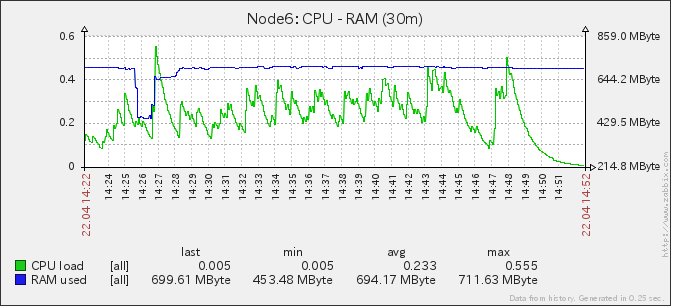
\includegraphics[width=1\hsize]{jdbc_aggregation_Testlauf_node6.png}
\caption{Auslastung des Knotens 6}
\end{figure}
\end{frame}

\begin{frame}\frametitle{Tests}
\begin{table}
\centering
\small
\begin{tabular}{|c|c|C{3cm}|}
\hline
\textbf{Durchschnittliche Antwortzeit} & \textbf{Aggregation} & \textbf{Aggregation mit Kartendarstellung} \\ \hline
\textbf{Postgres-XL} & 3,6s & 2,4s \\ \hline
\textbf{PostgreSQL} & 4,3s & 2,6s \\ \hline
\end{tabular}
\caption{Vergleich der Testergebnisse}
\end{table}

\begin{table}
\centering
\small
\begin{tabular}{|C{2.4cm}|c|C{2.9cm}|c|}
\hline
\textbf{Mittlere CPU Auslastung} & \textbf{Aggregation} & \textbf{Aggregation mit Kartendarstellung} & \textbf{Verarbeitung} \\ \hline
\textbf{Postgres-XL} & 0,2 & 0,1 & 0,5 \\ \hline
\textbf{PostgreSQL} & 3,6 & 0,4 & 0,5 \\ \hline	
\end{tabular}
\caption{Vergleich der CPU Auslastung, GTM VM nicht berücksichtigt}
\end{table}
\end{frame}

\section{Fazit}
%analog Thesis
 
\begin{frame}\frametitle{Fazit}
\begin{center}
Nutzwertanalyse mit Zeitverhalten und angepasster Wertung\\ % Außerdem wurde Wert für Dokumentation und Funktionsalität geändert
Nutzwert: 79
\end{center}
\begin{table}[h!]
\centering
\small
\begin{tabular}{|l|p{1.8cm}|l|p{1.8cm}|}
\hline
\textbf{Metrik} & \textbf{erreichter Wert} & \textbf{Erfüllung in \%} & \textbf{gewichteter Teilnutzen} \\ \hline
Interoperabilität & 12 & 100 & 20 \\ \hline
Funktionsumfang & 53 & 87 & 17 \\ \hline
Dokumentation & 8 & 69 & 10 \\ \hline
Zeitverhalten & 2 & 67 &  27 \\ \hline
Modifizierbarkeit & 5 & 100 & 5 \\ \hline
\end{tabular}
\caption{Neue Nutzwertanalyse von Postgres-XL}
\end{table}
\end{frame}
 
\begin{frame}\frametitle{Fazit}
\textbf{Ergebnisse:}\\
\begin{itemize}
\item Das Forschungsziel wurde erreicht
\item Postgres-XL ist für einen produktiven Einsatz nicht geeignet
\item Die Methodik ist geeignet für die Softwareauswahl%Nutzwertanalyse beschränkt aussagekräftig
\item Der Ist-Stand ist zu verbessern
\end{itemize}
\end{frame}
 
\begin{frame}\frametitle{Kolloquium}
\begin{center}
\textbf{Vielen Dank für Ihre Aufmerksamkeit!}
\end{center}
\end{frame} 
 
\begin{frame}\frametitle{}

\end{frame} 

\begin{frame}\frametitle{Ausgangsszenario}
\underline{Anforderungen an die Technologie:}
\begin{itemize}
\item PostgreSQL mit PostGIS zum Datenimport und -export nutzbar
\item Gruppierung und Filterung mit geringer Laufzeit
\item Parallele Berechnung über große Datenmengen mit geringer Laufzeit
\item Räumliche Berechnungen wie Verschneidung und Overlays
\item Nutzbare Schnittstelle zur Darstellung mit dem UMN MapServer
\end{itemize}
%funktionale und nicht-funktionale Anforderungen; technische Anforderungen
\end{frame}
 
\begin{frame}\frametitle{Qualität: Interoperabilität}
\begin{block}{Qualitätskriterium:}
Es sind Schnittstellen zur Ein- und Ausgabe vorhanden. Dabei soll es sich um PostgreSQL Import sowie PostgreSQL und UMN Export handeln.
\end{block}

\begin{block}{Qualitätsmetrik:}
Ist der Import und Export von räumlichen Daten aus PostgreSQL sowie eine Anbindungsmöglichkeit an den UMN.
Statische Abbildung:\\
$[Datenschnittstelle\ und\ UMN\ Schnittstelle\ vorhanden,$\\$Datenschnittstelle\ vorhanden,\ UMN\ Schnittstelle\ vorhanden,$\\$keine\ Schnittstelle\ vorhanden]\ nach\ [12,7,5,0]$
\end{block}
\end{frame} 

\begin{frame}\frametitle{Nutzwertanalyse}
\begin{table}
\begin{tabular}{|l|l|}
\hline
\textbf{Metrik} & \textbf{Gewichtung in \%} \\ \hline
%Richtigkeit & 10 \\ \hline
Interoperabilität & 30 \\ \hline
Funktionsumfang & 20 \\ \hline
%Fehlertoleranz & 8 \\ \hline
Dokumentation & 35 \\ \hline
%Zeitverhalten & 16 \\ \hline
Modifizierbarkeit & 15 \\ \hline
\end{tabular}
\caption{Wertungsmaßstab der einzelnen Metriken}
\end{table}

\begin{table}
\begin{tabular}{|l|l|}
\hline
\textbf{Metrik} & \textbf{Gewichtung in \%} \\ \hline
Interoperabilität & 20 \\ \hline
Funktionsumfang & 20 \\ \hline
Dokumentation & 15 \\ \hline
Zeitverhalten & 40 \\ \hline
Modifizierbarkeit & 5 \\ \hline
\end{tabular}
\caption{Neuer Wertungsmaßstab der einzelnen Metriken}
\end{table}
\end{frame}

\begin{frame}\frametitle{FT05}
\begin{figure}
\includegraphics[width=.5\textwidth]{../Abbildungen/2fields.png}
\caption[Kartenausschnitt mit 2 überlappenden Schlägen]{Kartenausschnitt mit 2 überlappenden Schlägen}
\end{figure}
\end{frame}

\begin{frame}\frametitle{FT05}
\setcounter{subfigure}{0}\begin{figure}
\begin{subfigure}{.3\textwidth}
  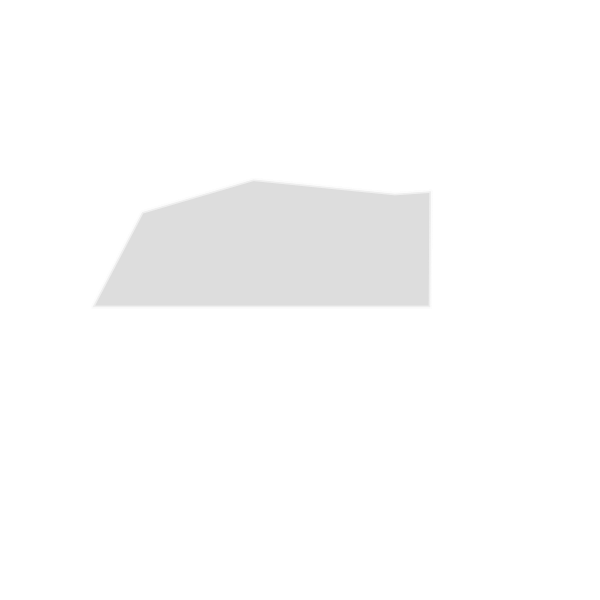
\includegraphics[width=.7\linewidth]{../Abbildungen/st_intersection.png}
  \caption{Intersection}
\end{subfigure}%
\begin{subfigure}{.3\textwidth}
  
\includegraphics[width=.7\linewidth]{../Abbildungen/st_union.png}
  \caption{Union}
\end{subfigure}
\begin{subfigure}{.3\textwidth}
  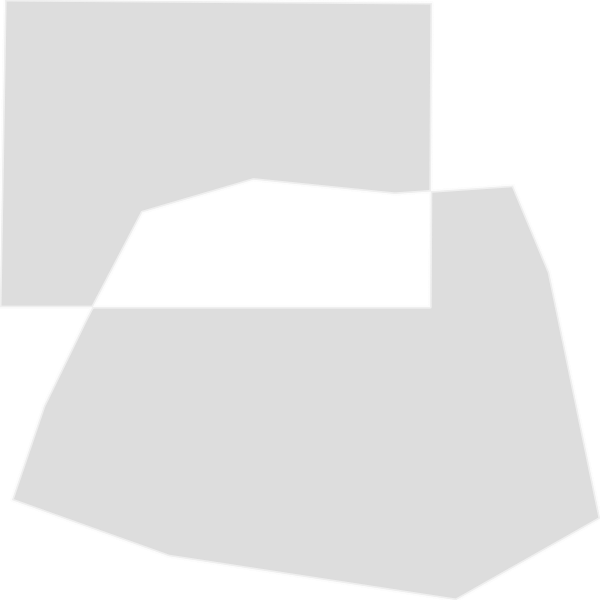
\includegraphics[width=.7\linewidth]{../Abbildungen/st_symdifference.png}
  \caption{Symmetric Difference}
\end{subfigure}
\caption{Ergebnisse der Verschneidungsfunktionen Intersection, Union und Symmetric Difference}
\end{figure}
\end{frame}

\begin{frame}\frametitle{FT05}
\setcounter{subfigure}{0}\begin{figure}
\begin{subfigure}{.5\textwidth}
  
\includegraphics[width=.7\linewidth]{../Abbildungen/st_difference1.png}
  \caption{Difference mit Schlag 1 zu Schlag 2}
\end{subfigure}%
\begin{subfigure}{.5\textwidth}
  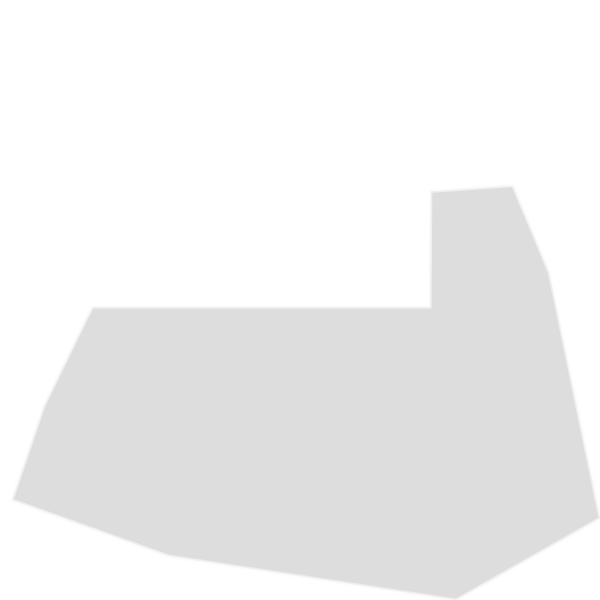
\includegraphics[width=.7\linewidth]{../Abbildungen/st_difference2.png}
  \caption{Difference mit Schlag 2 zu Schlag 1}
\end{subfigure}
\caption{Ergebnisse der Verschneidungsfunktionen Difference}
\end{figure}
\end{frame}
 
\begin{frame}\frametitle{Verarbeitung}
Interpolation mit Hilfe spezieller Algorithmen von Punkten zu Flächen.

\begin{block}{Probleme:}
\begin{itemize}
\item SQL Befehl $Insert\ Into$ ist nicht verwendbar
\item Die meisten Datensätzen konnten nicht verarbeitet werden
\item Nur ein Coordinator in Testläufen verwendbar
\item Keine Kontrolle der Ergebnisse
\end{itemize}
\end{block}
\end{frame} 

\end{document}
